\documentclass[twoside]{book}

% Packages required by doxygen
\usepackage{fixltx2e}
\usepackage{calc}
\usepackage{doxygen}
\usepackage[export]{adjustbox} % also loads graphicx
\usepackage{graphicx}
\usepackage[utf8]{inputenc}
\usepackage{makeidx}
\usepackage{multicol}
\usepackage{multirow}
\PassOptionsToPackage{warn}{textcomp}
\usepackage{textcomp}
\usepackage[nointegrals]{wasysym}
\usepackage[table]{xcolor}

% Font selection
\usepackage[T1]{fontenc}
\usepackage[scaled=.90]{helvet}
\usepackage{courier}
\usepackage{amssymb}
\usepackage{sectsty}
\renewcommand{\familydefault}{\sfdefault}
\allsectionsfont{%
  \fontseries{bc}\selectfont%
  \color{darkgray}%
}
\renewcommand{\DoxyLabelFont}{%
  \fontseries{bc}\selectfont%
  \color{darkgray}%
}
\newcommand{\+}{\discretionary{\mbox{\scriptsize$\hookleftarrow$}}{}{}}

% Page & text layout
\usepackage{geometry}
\geometry{%
  letterpaper,%
  top=2.5cm,%
  bottom=2.5cm,%
  left=2.5cm,%
  right=2.5cm%
}
\tolerance=750
\hfuzz=15pt
\hbadness=750
\setlength{\emergencystretch}{15pt}
\setlength{\parindent}{0cm}
\setlength{\parskip}{3ex plus 2ex minus 2ex}
\makeatletter
\renewcommand{\paragraph}{%
  \@startsection{paragraph}{4}{0ex}{-1.0ex}{1.0ex}{%
    \normalfont\normalsize\bfseries\SS@parafont%
  }%
}
\renewcommand{\subparagraph}{%
  \@startsection{subparagraph}{5}{0ex}{-1.0ex}{1.0ex}{%
    \normalfont\normalsize\bfseries\SS@subparafont%
  }%
}
\makeatother

% Headers & footers
\usepackage{fancyhdr}
\pagestyle{fancyplain}
\fancyhead[LE]{\fancyplain{}{\bfseries\thepage}}
\fancyhead[CE]{\fancyplain{}{}}
\fancyhead[RE]{\fancyplain{}{\bfseries\leftmark}}
\fancyhead[LO]{\fancyplain{}{\bfseries\rightmark}}
\fancyhead[CO]{\fancyplain{}{}}
\fancyhead[RO]{\fancyplain{}{\bfseries\thepage}}
\fancyfoot[LE]{\fancyplain{}{}}
\fancyfoot[CE]{\fancyplain{}{}}
\fancyfoot[RE]{\fancyplain{}{\bfseries\scriptsize Generated by Doxygen }}
\fancyfoot[LO]{\fancyplain{}{\bfseries\scriptsize Generated by Doxygen }}
\fancyfoot[CO]{\fancyplain{}{}}
\fancyfoot[RO]{\fancyplain{}{}}
\renewcommand{\footrulewidth}{0.4pt}
\renewcommand{\chaptermark}[1]{%
  \markboth{#1}{}%
}
\renewcommand{\sectionmark}[1]{%
  \markright{\thesection\ #1}%
}

% Indices & bibliography
\usepackage{natbib}
\usepackage[titles]{tocloft}
\setcounter{tocdepth}{3}
\setcounter{secnumdepth}{5}
\makeindex

% Hyperlinks (required, but should be loaded last)
\usepackage{ifpdf}
\ifpdf
  \usepackage[pdftex,pagebackref=true]{hyperref}
\else
  \usepackage[ps2pdf,pagebackref=true]{hyperref}
\fi
\hypersetup{%
  colorlinks=true,%
  linkcolor=blue,%
  citecolor=blue,%
  unicode%
}

% Custom commands
\newcommand{\clearemptydoublepage}{%
  \newpage{\pagestyle{empty}\cleardoublepage}%
}

\usepackage{caption}
\captionsetup{labelsep=space,justification=centering,font={bf},singlelinecheck=off,skip=4pt,position=top}

%===== C O N T E N T S =====

\begin{document}

% Titlepage & ToC
\hypersetup{pageanchor=false,
             bookmarksnumbered=true,
             pdfencoding=unicode
            }
\pagenumbering{alph}
\begin{titlepage}
\vspace*{7cm}
\begin{center}%
{\Large sample\+S\+N\+Ps \\[1ex]\large 0.\+9 }\\
\vspace*{1cm}
{\large Generated by Doxygen 1.8.13}\\
\end{center}
\end{titlepage}
\clearemptydoublepage
\pagenumbering{roman}
\tableofcontents
\clearemptydoublepage
\pagenumbering{arabic}
\hypersetup{pageanchor=true}

%--- Begin generated contents ---
\chapter{Overview}
\label{index}\hypertarget{index}{}This distribution consists of three parts. One, a program ({\itshape sample\+S\+N\+Ps}) that creates and saves ordered random samples of S\+N\+Ps from a variety of formats. Two, a program ({\itshape sample\+LD}) that calculates linkage disequilibrium (LD) among randomly chosen (without replacement) pairs of S\+N\+Ps from a \href{http://zzz.bwh.harvard.edu/plink/data.shtml#bed}{\tt binary variant format file}. Three, a library ({\itshape libsamp\+Files.\+a}) that allows users to build similar applications taking advantage of the fast sampling algorithms used in the two programs mentioned above.

\section*{Requirements}

The software is build for Unix-\/like systems. Neither compilation nor running was checked under Windows and there are reasons to believe it will not compile on that OS. There are no dependencies other than a compiler that understands the C++11 standard. Random number generation employs the {\ttfamily R\+D\+R\+A\+ND} C\+PU instruction if supported by the processor, otherwise an implementation of the 64-\/bit Mersenne Twister \cite{matsumoto98a} is substituted. Intel Ivy Bridge or later support {\ttfamily R\+D\+R\+A\+ND}. With A\+MD it is not completely clear. Opteron definitely does not support it. Zen architectures (Ryzen) claim to support it, but I did not have access to one so I cannot personally vouch for it. The R\+NG choice is made automatically at run time.

\section*{Installation}

The simplest way to install everything is to run \begin{DoxyVerb}make all
sudo make install
\end{DoxyVerb}


in the directory with the source code. This will install the executables ({\itshape sample\+S\+N\+Ps} and {\itshape sample\+LD}) in \+\_\+/usr/local/bin/\+\_\+ and the library in the appropriate folders in \+\_\+/usr/local/\+\_\+. The included Makefile can be modified to change where things go. The headers {\itshape \hyperlink{varfiles_8hpp}{varfiles.\+hpp}}, {\itshape \hyperlink{populations_8hpp}{populations.\+hpp}}, and {\itshape \hyperlink{random_8hpp}{random.\+hpp}} have to be included in your code as necessary.

\section*{Testing}

The {\itshape tests/} directory contains example .bed, .tped, .vcf, and .hmp.\+txt files to try running the programs on. To keep sizes manageable for distribution, the .bed file has 50,000 loci, while the text files have only 5,000. Make sure your samples do not exceed these values. Uncompress the directory and run, for example, \begin{DoxyVerb}./sampleSNPs -i tests/sample -t BED -s 5000
\end{DoxyVerb}


This should sample 5,000 S\+N\+Ps from the included {\itshape sample\+\_\+\+A\+L\+L.\+bed} and {\itshape sample\+\_\+\+A\+L\+L.\+bim} files and save the results into files with the {\itshape sample\+\_\+\+A\+L\+L\+\_\+s5000} prefix.

Note that {\itshape sample\+LD} supports only the .bed format.

Running {\itshape sample\+S\+N\+Ps} and {\itshape sample\+LD} without flags will cause these programs to print flag descriptions and exit.

\section*{Timing}

Expanding the {\itshape timing\+Trials.\+tar.\+gz} archive will generate a directory with separate software, depending only on \hyperlink{random_8cpp}{random.\+cpp} and .hpp, that performs analyses of execution time using Vitter\textquotesingle{}s Method D and Method S. There is a R\+E\+A\+D\+M\+E.\+md file that explains how to compile and run these analyses. 
\chapter{Hierarchical Index}
\section{Class Hierarchy}
This inheritance list is sorted roughly, but not completely, alphabetically\+:\begin{DoxyCompactList}
\item \contentsline{section}{samp\+Files\+:\+:Generate}{\pageref{classsamp_files_1_1_generate}}{}
\begin{DoxyCompactList}
\item \contentsline{section}{samp\+Files\+:\+:Generate\+HR}{\pageref{classsamp_files_1_1_generate_h_r}}{}
\item \contentsline{section}{samp\+Files\+:\+:Generate\+MT}{\pageref{classsamp_files_1_1_generate_m_t}}{}
\end{DoxyCompactList}
\item \contentsline{section}{samp\+Files\+:\+:Pop\+Index}{\pageref{classsamp_files_1_1_pop_index}}{}
\item \contentsline{section}{samp\+Files\+:\+:Ran\+Draw}{\pageref{classsamp_files_1_1_ran_draw}}{}
\item \contentsline{section}{samp\+Files\+:\+:Var\+File}{\pageref{classsamp_files_1_1_var_file}}{}
\begin{DoxyCompactList}
\item \contentsline{section}{samp\+Files\+:\+:Gbin\+File}{\pageref{classsamp_files_1_1_gbin_file}}{}
\begin{DoxyCompactList}
\item \contentsline{section}{samp\+Files\+:\+:Bed\+File}{\pageref{classsamp_files_1_1_bed_file}}{}
\begin{DoxyCompactList}
\item \contentsline{section}{samp\+Files\+:\+:Bed\+FileI}{\pageref{classsamp_files_1_1_bed_file_i}}{}
\item \contentsline{section}{samp\+Files\+:\+:Bed\+FileO}{\pageref{classsamp_files_1_1_bed_file_o}}{}
\end{DoxyCompactList}
\item \contentsline{section}{samp\+Files\+:\+:Gbin\+FileI}{\pageref{classsamp_files_1_1_gbin_file_i}}{}
\item \contentsline{section}{samp\+Files\+:\+:Gbin\+FileO}{\pageref{classsamp_files_1_1_gbin_file_o}}{}
\end{DoxyCompactList}
\item \contentsline{section}{samp\+Files\+:\+:Gtxt\+File}{\pageref{classsamp_files_1_1_gtxt_file}}{}
\begin{DoxyCompactList}
\item \contentsline{section}{samp\+Files\+:\+:Gtxt\+FileI}{\pageref{classsamp_files_1_1_gtxt_file_i}}{}
\item \contentsline{section}{samp\+Files\+:\+:Gtxt\+FileO}{\pageref{classsamp_files_1_1_gtxt_file_o}}{}
\item \contentsline{section}{samp\+Files\+:\+:Hmp\+File}{\pageref{classsamp_files_1_1_hmp_file}}{}
\begin{DoxyCompactList}
\item \contentsline{section}{samp\+Files\+:\+:Hmp\+FileI}{\pageref{classsamp_files_1_1_hmp_file_i}}{}
\item \contentsline{section}{samp\+Files\+:\+:Hmp\+FileO}{\pageref{classsamp_files_1_1_hmp_file_o}}{}
\end{DoxyCompactList}
\item \contentsline{section}{samp\+Files\+:\+:Tped\+File}{\pageref{classsamp_files_1_1_tped_file}}{}
\begin{DoxyCompactList}
\item \contentsline{section}{samp\+Files\+:\+:Tped\+FileI}{\pageref{classsamp_files_1_1_tped_file_i}}{}
\item \contentsline{section}{samp\+Files\+:\+:Tped\+FileO}{\pageref{classsamp_files_1_1_tped_file_o}}{}
\end{DoxyCompactList}
\item \contentsline{section}{samp\+Files\+:\+:Vcf\+File}{\pageref{classsamp_files_1_1_vcf_file}}{}
\begin{DoxyCompactList}
\item \contentsline{section}{samp\+Files\+:\+:Vcf\+FileI}{\pageref{classsamp_files_1_1_vcf_file_i}}{}
\item \contentsline{section}{samp\+Files\+:\+:Vcf\+FileO}{\pageref{classsamp_files_1_1_vcf_file_o}}{}
\end{DoxyCompactList}
\end{DoxyCompactList}
\end{DoxyCompactList}
\end{DoxyCompactList}

\chapter{Class Index}
\section{Class List}
Here are the classes, structs, unions and interfaces with brief descriptions\+:\begin{DoxyCompactList}
\item\contentsline{section}{\hyperlink{classsamp_files_1_1_bed_file}{samp\+Files\+::\+Bed\+File} \\*B\+ED file base class }{\pageref{classsamp_files_1_1_bed_file}}{}
\item\contentsline{section}{\hyperlink{classsamp_files_1_1_bed_file_i}{samp\+Files\+::\+Bed\+FileI} \\*B\+ED file input class }{\pageref{classsamp_files_1_1_bed_file_i}}{}
\item\contentsline{section}{\hyperlink{classsamp_files_1_1_bed_file_o}{samp\+Files\+::\+Bed\+FileO} \\*B\+ED file output class }{\pageref{classsamp_files_1_1_bed_file_o}}{}
\item\contentsline{section}{\hyperlink{classsamp_files_1_1_gbin_file}{samp\+Files\+::\+Gbin\+File} \\*Generic binary file base class }{\pageref{classsamp_files_1_1_gbin_file}}{}
\item\contentsline{section}{\hyperlink{classsamp_files_1_1_gbin_file_i}{samp\+Files\+::\+Gbin\+FileI} \\*Binary file input class }{\pageref{classsamp_files_1_1_gbin_file_i}}{}
\item\contentsline{section}{\hyperlink{classsamp_files_1_1_gbin_file_o}{samp\+Files\+::\+Gbin\+FileO} \\*Generic binary file output class }{\pageref{classsamp_files_1_1_gbin_file_o}}{}
\item\contentsline{section}{\hyperlink{classsamp_files_1_1_generate}{samp\+Files\+::\+Generate} \\*Abstract base random number class }{\pageref{classsamp_files_1_1_generate}}{}
\item\contentsline{section}{\hyperlink{classsamp_files_1_1_generate_h_r}{samp\+Files\+::\+Generate\+HR} \\*Hardware random number generating class }{\pageref{classsamp_files_1_1_generate_h_r}}{}
\item\contentsline{section}{\hyperlink{classsamp_files_1_1_generate_m_t}{samp\+Files\+::\+Generate\+MT} \\*Pseudo-\/random number generator }{\pageref{classsamp_files_1_1_generate_m_t}}{}
\item\contentsline{section}{\hyperlink{classsamp_files_1_1_gtxt_file}{samp\+Files\+::\+Gtxt\+File} \\*Generic text file base class }{\pageref{classsamp_files_1_1_gtxt_file}}{}
\item\contentsline{section}{\hyperlink{classsamp_files_1_1_gtxt_file_i}{samp\+Files\+::\+Gtxt\+FileI} \\*Text file input class }{\pageref{classsamp_files_1_1_gtxt_file_i}}{}
\item\contentsline{section}{\hyperlink{classsamp_files_1_1_gtxt_file_o}{samp\+Files\+::\+Gtxt\+FileO} \\*Generic text file output class }{\pageref{classsamp_files_1_1_gtxt_file_o}}{}
\item\contentsline{section}{\hyperlink{classsamp_files_1_1_hmp_file}{samp\+Files\+::\+Hmp\+File} \\*Hapmap (H\+MP) file base class }{\pageref{classsamp_files_1_1_hmp_file}}{}
\item\contentsline{section}{\hyperlink{classsamp_files_1_1_hmp_file_i}{samp\+Files\+::\+Hmp\+FileI} \\*H\+MP file input class }{\pageref{classsamp_files_1_1_hmp_file_i}}{}
\item\contentsline{section}{\hyperlink{classsamp_files_1_1_hmp_file_o}{samp\+Files\+::\+Hmp\+FileO} \\*H\+MP file output class }{\pageref{classsamp_files_1_1_hmp_file_o}}{}
\item\contentsline{section}{\hyperlink{classsamp_files_1_1_pop_index}{samp\+Files\+::\+Pop\+Index} \\*Population index }{\pageref{classsamp_files_1_1_pop_index}}{}
\item\contentsline{section}{\hyperlink{classsamp_files_1_1_ran_draw}{samp\+Files\+::\+Ran\+Draw} \\*Random number generating class }{\pageref{classsamp_files_1_1_ran_draw}}{}
\item\contentsline{section}{\hyperlink{classsamp_files_1_1_tped_file}{samp\+Files\+::\+Tped\+File} \\*T\+P\+ED file base class }{\pageref{classsamp_files_1_1_tped_file}}{}
\item\contentsline{section}{\hyperlink{classsamp_files_1_1_tped_file_i}{samp\+Files\+::\+Tped\+FileI} \\*T\+P\+ED file input class }{\pageref{classsamp_files_1_1_tped_file_i}}{}
\item\contentsline{section}{\hyperlink{classsamp_files_1_1_tped_file_o}{samp\+Files\+::\+Tped\+FileO} \\*T\+P\+ED file output class }{\pageref{classsamp_files_1_1_tped_file_o}}{}
\item\contentsline{section}{\hyperlink{classsamp_files_1_1_var_file}{samp\+Files\+::\+Var\+File} \\*Base variant file class }{\pageref{classsamp_files_1_1_var_file}}{}
\item\contentsline{section}{\hyperlink{classsamp_files_1_1_vcf_file}{samp\+Files\+::\+Vcf\+File} \\*V\+CF file base class }{\pageref{classsamp_files_1_1_vcf_file}}{}
\item\contentsline{section}{\hyperlink{classsamp_files_1_1_vcf_file_i}{samp\+Files\+::\+Vcf\+FileI} \\*V\+CF file input class }{\pageref{classsamp_files_1_1_vcf_file_i}}{}
\item\contentsline{section}{\hyperlink{classsamp_files_1_1_vcf_file_o}{samp\+Files\+::\+Vcf\+FileO} \\*V\+CF file output class }{\pageref{classsamp_files_1_1_vcf_file_o}}{}
\end{DoxyCompactList}

\chapter{File Index}
\section{File List}
Here is a list of all documented files with brief descriptions\+:\begin{DoxyCompactList}
\item\contentsline{section}{\hyperlink{populations_8cpp}{populations.\+cpp} \\*Connect lines with populations }{\pageref{populations_8cpp}}{}
\item\contentsline{section}{\hyperlink{populations_8hpp}{populations.\+hpp} \\*Connect lines with populations }{\pageref{populations_8hpp}}{}
\item\contentsline{section}{\hyperlink{random_8cpp}{random.\+cpp} \\*Random number generation }{\pageref{random_8cpp}}{}
\item\contentsline{section}{\hyperlink{random_8hpp}{random.\+hpp} \\*Random number generation }{\pageref{random_8hpp}}{}
\item\contentsline{section}{\hyperlink{sample_l_d_8cpp}{sample\+L\+D.\+cpp} \\*Sample-\/based linkage disequilibrium }{\pageref{sample_l_d_8cpp}}{}
\item\contentsline{section}{\hyperlink{sample_s_n_ps_8cpp}{sample\+S\+N\+Ps.\+cpp} \\*Sample S\+N\+Ps }{\pageref{sample_s_n_ps_8cpp}}{}
\item\contentsline{section}{\hyperlink{varfiles_8cpp}{varfiles.\+cpp} \\*Read and write genetic variant files }{\pageref{varfiles_8cpp}}{}
\item\contentsline{section}{\hyperlink{varfiles_8hpp}{varfiles.\+hpp} \\*Read and write genetic variant files }{\pageref{varfiles_8hpp}}{}
\end{DoxyCompactList}

\chapter{Class Documentation}
\hypertarget{classsamp_files_1_1_bed_file}{}\section{samp\+Files\+:\+:Bed\+File Class Reference}
\label{classsamp_files_1_1_bed_file}\index{samp\+Files\+::\+Bed\+File@{samp\+Files\+::\+Bed\+File}}


B\+ED file base class.  




{\ttfamily \#include $<$varfiles.\+hpp$>$}



Inheritance diagram for samp\+Files\+:\+:Bed\+File\+:\nopagebreak
\begin{figure}[H]
\begin{center}
\leavevmode
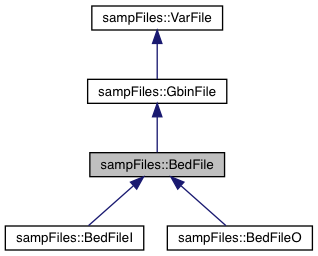
\includegraphics[width=310pt]{classsamp_files_1_1_bed_file__inherit__graph}
\end{center}
\end{figure}


Collaboration diagram for samp\+Files\+:\+:Bed\+File\+:\nopagebreak
\begin{figure}[H]
\begin{center}
\leavevmode
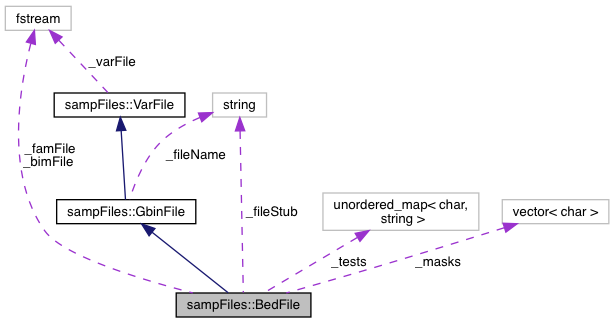
\includegraphics[width=350pt]{classsamp_files_1_1_bed_file__coll__graph}
\end{center}
\end{figure}
\subsection*{Public Member Functions}
\begin{DoxyCompactItemize}
\item 
\mbox{\Hypertarget{classsamp_files_1_1_bed_file_a0853371d06c87876859d5cf3c711c8e3}\label{classsamp_files_1_1_bed_file_a0853371d06c87876859d5cf3c711c8e3}} 
\hyperlink{classsamp_files_1_1_bed_file_a0853371d06c87876859d5cf3c711c8e3}{Bed\+File} ()
\begin{DoxyCompactList}\small\item\em Default constructor. \end{DoxyCompactList}\item 
\hyperlink{classsamp_files_1_1_bed_file_a69631d96080c22e686e8acb75cf2cc89}{Bed\+File} (const string \&stub\+Name)
\begin{DoxyCompactList}\small\item\em File name constructor. \end{DoxyCompactList}\item 
\mbox{\Hypertarget{classsamp_files_1_1_bed_file_a77703bfb5a3a3392e71514a41c5bde1c}\label{classsamp_files_1_1_bed_file_a77703bfb5a3a3392e71514a41c5bde1c}} 
\hyperlink{classsamp_files_1_1_bed_file_a77703bfb5a3a3392e71514a41c5bde1c}{Bed\+File} (const \hyperlink{classsamp_files_1_1_bed_file}{Bed\+File} \&in)=default
\begin{DoxyCompactList}\small\item\em Copy constructor. \end{DoxyCompactList}\item 
\mbox{\Hypertarget{classsamp_files_1_1_bed_file_ad2f3aa3c098034139fa371f65dadfd50}\label{classsamp_files_1_1_bed_file_ad2f3aa3c098034139fa371f65dadfd50}} 
\hyperlink{classsamp_files_1_1_bed_file}{Bed\+File} \& \hyperlink{classsamp_files_1_1_bed_file_ad2f3aa3c098034139fa371f65dadfd50}{operator=} (const \hyperlink{classsamp_files_1_1_bed_file}{Bed\+File} \&in)=default
\begin{DoxyCompactList}\small\item\em Copy assignment. \end{DoxyCompactList}\item 
\mbox{\Hypertarget{classsamp_files_1_1_bed_file_a615dcf39c6d51a5ff40df4631873b5ab}\label{classsamp_files_1_1_bed_file_a615dcf39c6d51a5ff40df4631873b5ab}} 
\hyperlink{classsamp_files_1_1_bed_file_a615dcf39c6d51a5ff40df4631873b5ab}{Bed\+File} (\hyperlink{classsamp_files_1_1_bed_file}{Bed\+File} \&\&in)=default
\begin{DoxyCompactList}\small\item\em Move constructor. \end{DoxyCompactList}\item 
\mbox{\Hypertarget{classsamp_files_1_1_bed_file_af43a7be226fcdd6898fba4b0b508395c}\label{classsamp_files_1_1_bed_file_af43a7be226fcdd6898fba4b0b508395c}} 
\hyperlink{classsamp_files_1_1_bed_file}{Bed\+File} \& \hyperlink{classsamp_files_1_1_bed_file_af43a7be226fcdd6898fba4b0b508395c}{operator=} (\hyperlink{classsamp_files_1_1_bed_file}{Bed\+File} \&\&in)=default
\begin{DoxyCompactList}\small\item\em Move assignment. \end{DoxyCompactList}\item 
\mbox{\Hypertarget{classsamp_files_1_1_bed_file_a8e6b512579968f51763ac693c1c4432b}\label{classsamp_files_1_1_bed_file_a8e6b512579968f51763ac693c1c4432b}} 
\hyperlink{classsamp_files_1_1_bed_file_a8e6b512579968f51763ac693c1c4432b}{$\sim$\+Bed\+File} ()
\begin{DoxyCompactList}\small\item\em Destructor. \end{DoxyCompactList}\item 
\mbox{\Hypertarget{classsamp_files_1_1_bed_file_a7e0c3fcc90545d7ff69eeaec6c0ac6f3}\label{classsamp_files_1_1_bed_file_a7e0c3fcc90545d7ff69eeaec6c0ac6f3}} 
virtual void \hyperlink{classsamp_files_1_1_bed_file_a7e0c3fcc90545d7ff69eeaec6c0ac6f3}{open} ()
\begin{DoxyCompactList}\small\item\em Open stream (does nothing) \end{DoxyCompactList}\item 
\mbox{\Hypertarget{classsamp_files_1_1_bed_file_acc8796c6ea50710287b0e2117c4b381e}\label{classsamp_files_1_1_bed_file_acc8796c6ea50710287b0e2117c4b381e}} 
void \hyperlink{classsamp_files_1_1_bed_file_acc8796c6ea50710287b0e2117c4b381e}{close} ()
\begin{DoxyCompactList}\small\item\em Close stream. \end{DoxyCompactList}\end{DoxyCompactItemize}
\subsection*{Protected Attributes}
\begin{DoxyCompactItemize}
\item 
\mbox{\Hypertarget{classsamp_files_1_1_bed_file_a4ff2286fc39ccc3eaa57f70d27d6947a}\label{classsamp_files_1_1_bed_file_a4ff2286fc39ccc3eaa57f70d27d6947a}} 
fstream \hyperlink{classsamp_files_1_1_bed_file_a4ff2286fc39ccc3eaa57f70d27d6947a}{\+\_\+fam\+File}
\begin{DoxyCompactList}\small\item\em Corresponding .fam file stream. \end{DoxyCompactList}\item 
\mbox{\Hypertarget{classsamp_files_1_1_bed_file_aa7b6f84a9bf506e239dbbbf1c03ce13a}\label{classsamp_files_1_1_bed_file_aa7b6f84a9bf506e239dbbbf1c03ce13a}} 
fstream \hyperlink{classsamp_files_1_1_bed_file_aa7b6f84a9bf506e239dbbbf1c03ce13a}{\+\_\+bim\+File}
\begin{DoxyCompactList}\small\item\em Corresponding .bim file stream. \end{DoxyCompactList}\item 
\mbox{\Hypertarget{classsamp_files_1_1_bed_file_a2d2ec10c5653c4bd957351a8ff5226be}\label{classsamp_files_1_1_bed_file_a2d2ec10c5653c4bd957351a8ff5226be}} 
string \hyperlink{classsamp_files_1_1_bed_file_a2d2ec10c5653c4bd957351a8ff5226be}{\+\_\+file\+Stub}
\begin{DoxyCompactList}\small\item\em File name stub (minus the extension) \end{DoxyCompactList}\end{DoxyCompactItemize}
\subsection*{Static Protected Attributes}
\begin{DoxyCompactItemize}
\item 
static const vector$<$ char $>$ \hyperlink{classsamp_files_1_1_bed_file_a26fc3857dd112e96e626da1a48b026bc}{\+\_\+masks} = \{static\+\_\+cast$<$char$>$(0x03), static\+\_\+cast$<$char$>$(0x0\+C), static\+\_\+cast$<$char$>$(0x30), static\+\_\+cast$<$char$>$(0x\+C0)\}
\begin{DoxyCompactList}\small\item\em Genotype bit masks. \end{DoxyCompactList}\item 
static const unordered\+\_\+map$<$ char, string $>$ \hyperlink{classsamp_files_1_1_bed_file_a153af12f613ef8cdea6297e124b92de7}{\+\_\+tests}
\begin{DoxyCompactList}\small\item\em Genotype bit tests. \end{DoxyCompactList}\end{DoxyCompactItemize}
\subsection*{Additional Inherited Members}


\subsection{Detailed Description}
B\+ED file base class. 

Sets up streams for the auxiliary files. 

\subsection{Constructor \& Destructor Documentation}
\mbox{\Hypertarget{classsamp_files_1_1_bed_file_a69631d96080c22e686e8acb75cf2cc89}\label{classsamp_files_1_1_bed_file_a69631d96080c22e686e8acb75cf2cc89}} 
\index{samp\+Files\+::\+Bed\+File@{samp\+Files\+::\+Bed\+File}!Bed\+File@{Bed\+File}}
\index{Bed\+File@{Bed\+File}!samp\+Files\+::\+Bed\+File@{samp\+Files\+::\+Bed\+File}}
\subsubsection{\texorpdfstring{Bed\+File()}{BedFile()}}
{\footnotesize\ttfamily Bed\+File\+::\+Bed\+File (\begin{DoxyParamCaption}\item[{const string \&}]{stub\+Name }\end{DoxyParamCaption})}



File name constructor. 


\begin{DoxyParams}[1]{Parameters}
\mbox{\tt in}  & {\em stub\+Name} & file name minus the extension \\
\hline
\end{DoxyParams}


\subsection{Member Data Documentation}
\mbox{\Hypertarget{classsamp_files_1_1_bed_file_a26fc3857dd112e96e626da1a48b026bc}\label{classsamp_files_1_1_bed_file_a26fc3857dd112e96e626da1a48b026bc}} 
\index{samp\+Files\+::\+Bed\+File@{samp\+Files\+::\+Bed\+File}!\+\_\+masks@{\+\_\+masks}}
\index{\+\_\+masks@{\+\_\+masks}!samp\+Files\+::\+Bed\+File@{samp\+Files\+::\+Bed\+File}}
\subsubsection{\texorpdfstring{\+\_\+masks}{\_masks}}
{\footnotesize\ttfamily const vector$<$ char $>$ Bed\+File\+::\+\_\+masks = \{static\+\_\+cast$<$char$>$(0x03), static\+\_\+cast$<$char$>$(0x0\+C), static\+\_\+cast$<$char$>$(0x30), static\+\_\+cast$<$char$>$(0x\+C0)\}\hspace{0.3cm}{\ttfamily [static]}, {\ttfamily [protected]}}



Genotype bit masks. 

Used to isolate each of the four genotypes (moving from the last bit pair) from the .bed two-\/bit genotype coding. \mbox{\Hypertarget{classsamp_files_1_1_bed_file_a153af12f613ef8cdea6297e124b92de7}\label{classsamp_files_1_1_bed_file_a153af12f613ef8cdea6297e124b92de7}} 
\index{samp\+Files\+::\+Bed\+File@{samp\+Files\+::\+Bed\+File}!\+\_\+tests@{\+\_\+tests}}
\index{\+\_\+tests@{\+\_\+tests}!samp\+Files\+::\+Bed\+File@{samp\+Files\+::\+Bed\+File}}
\subsubsection{\texorpdfstring{\+\_\+tests}{\_tests}}
{\footnotesize\ttfamily const unordered\+\_\+map$<$ char, string $>$ Bed\+File\+::\+\_\+tests\hspace{0.3cm}{\ttfamily [static]}, {\ttfamily [protected]}}

{\bfseries Initial value\+:}
\begin{DoxyCode}
= \{
    \{\textcolor{charliteral}{'M'}, \{\textcolor{keyword}{static\_cast<}\textcolor{keywordtype}{char}\textcolor{keyword}{>}(0x01), static\_cast<char>(0x04), \textcolor{keyword}{static\_cast<}\textcolor{keywordtype}{char}\textcolor{keyword}{>}(0x10), static\_cast<char>(0
      x40)\}\},
    \{\textcolor{charliteral}{'H'}, \{\textcolor{keyword}{static\_cast<}\textcolor{keywordtype}{char}\textcolor{keyword}{>}(0x02), static\_cast<char>(0x08), \textcolor{keyword}{static\_cast<}\textcolor{keywordtype}{char}\textcolor{keyword}{>}(0x20), static\_cast<char>(0
      x80)\}\}
\}
\end{DoxyCode}


Genotype bit tests. 

Used to test each of the four genotypes (moving from the last bit pair) from the .bed two-\/bit genotype coding for the possible states. 

The documentation for this class was generated from the following files\+:\begin{DoxyCompactItemize}
\item 
\hyperlink{varfiles_8hpp}{varfiles.\+hpp}\item 
\hyperlink{varfiles_8cpp}{varfiles.\+cpp}\end{DoxyCompactItemize}

\hypertarget{classsamp_files_1_1_bed_file_i}{}\section{samp\+Files\+:\+:Bed\+FileI Class Reference}
\label{classsamp_files_1_1_bed_file_i}\index{samp\+Files\+::\+Bed\+FileI@{samp\+Files\+::\+Bed\+FileI}}


B\+ED file input class.  




{\ttfamily \#include $<$varfiles.\+hpp$>$}



Inheritance diagram for samp\+Files\+:\+:Bed\+FileI\+:\nopagebreak
\begin{figure}[H]
\begin{center}
\leavevmode
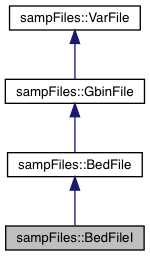
\includegraphics[width=184pt]{classsamp_files_1_1_bed_file_i__inherit__graph}
\end{center}
\end{figure}


Collaboration diagram for samp\+Files\+:\+:Bed\+FileI\+:\nopagebreak
\begin{figure}[H]
\begin{center}
\leavevmode
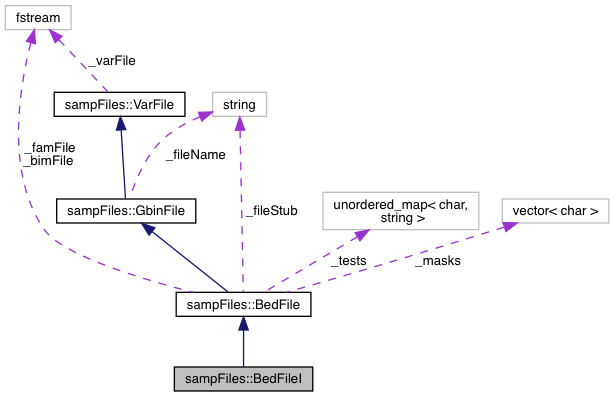
\includegraphics[width=350pt]{classsamp_files_1_1_bed_file_i__coll__graph}
\end{center}
\end{figure}
\subsection*{Public Member Functions}
\begin{DoxyCompactItemize}
\item 
\mbox{\Hypertarget{classsamp_files_1_1_bed_file_i_a8199fdbd94df701b0de0cbab46cddbed}\label{classsamp_files_1_1_bed_file_i_a8199fdbd94df701b0de0cbab46cddbed}} 
\hyperlink{classsamp_files_1_1_bed_file_i_a8199fdbd94df701b0de0cbab46cddbed}{Bed\+FileI} ()
\begin{DoxyCompactList}\small\item\em Default constructor. \end{DoxyCompactList}\item 
\hyperlink{classsamp_files_1_1_bed_file_i_abb33c9b143ab40ee37b56a62e7e999f8}{Bed\+FileI} (const string \&stub\+Name)
\begin{DoxyCompactList}\small\item\em File name constructor. \end{DoxyCompactList}\item 
\mbox{\Hypertarget{classsamp_files_1_1_bed_file_i_ae7aaf5d849475010fd5f9d1154a18b34}\label{classsamp_files_1_1_bed_file_i_ae7aaf5d849475010fd5f9d1154a18b34}} 
\hyperlink{classsamp_files_1_1_bed_file_i_ae7aaf5d849475010fd5f9d1154a18b34}{Bed\+FileI} (const \hyperlink{classsamp_files_1_1_bed_file_i}{Bed\+FileI} \&in)=default
\begin{DoxyCompactList}\small\item\em Copy constructor. \end{DoxyCompactList}\item 
\mbox{\Hypertarget{classsamp_files_1_1_bed_file_i_a720c177b75980289a6eb9cfb2564ba2f}\label{classsamp_files_1_1_bed_file_i_a720c177b75980289a6eb9cfb2564ba2f}} 
\hyperlink{classsamp_files_1_1_bed_file_i}{Bed\+FileI} \& \hyperlink{classsamp_files_1_1_bed_file_i_a720c177b75980289a6eb9cfb2564ba2f}{operator=} (const \hyperlink{classsamp_files_1_1_bed_file_i}{Bed\+FileI} \&in)=default
\begin{DoxyCompactList}\small\item\em Copy assignment. \end{DoxyCompactList}\item 
\mbox{\Hypertarget{classsamp_files_1_1_bed_file_i_ad22ff60c09b7fd0d64f5866451f2d861}\label{classsamp_files_1_1_bed_file_i_ad22ff60c09b7fd0d64f5866451f2d861}} 
\hyperlink{classsamp_files_1_1_bed_file_i_ad22ff60c09b7fd0d64f5866451f2d861}{Bed\+FileI} (\hyperlink{classsamp_files_1_1_bed_file_i}{Bed\+FileI} \&\&in)=default
\begin{DoxyCompactList}\small\item\em Move constructor. \end{DoxyCompactList}\item 
\mbox{\Hypertarget{classsamp_files_1_1_bed_file_i_a9c99aae36f0c6d710f7940affe35cf58}\label{classsamp_files_1_1_bed_file_i_a9c99aae36f0c6d710f7940affe35cf58}} 
\hyperlink{classsamp_files_1_1_bed_file_i}{Bed\+FileI} \& \hyperlink{classsamp_files_1_1_bed_file_i_a9c99aae36f0c6d710f7940affe35cf58}{operator=} (\hyperlink{classsamp_files_1_1_bed_file_i}{Bed\+FileI} \&\&in)=default
\begin{DoxyCompactList}\small\item\em Move assignment. \end{DoxyCompactList}\item 
\mbox{\Hypertarget{classsamp_files_1_1_bed_file_i_a87823c162cc37744aba01c6617ff682e}\label{classsamp_files_1_1_bed_file_i_a87823c162cc37744aba01c6617ff682e}} 
\hyperlink{classsamp_files_1_1_bed_file_i_a87823c162cc37744aba01c6617ff682e}{$\sim$\+Bed\+FileI} ()
\begin{DoxyCompactList}\small\item\em Destructor. \end{DoxyCompactList}\item 
\mbox{\Hypertarget{classsamp_files_1_1_bed_file_i_a36ff04242d3c4bd65c9f1d8be5153997}\label{classsamp_files_1_1_bed_file_i_a36ff04242d3c4bd65c9f1d8be5153997}} 
void \hyperlink{classsamp_files_1_1_bed_file_i_a36ff04242d3c4bd65c9f1d8be5153997}{open} ()
\begin{DoxyCompactList}\small\item\em Open stream to read. \end{DoxyCompactList}\item 
void \hyperlink{classsamp_files_1_1_bed_file_i_ac1050b3b8aec9108ae05285cbdfd85b3}{sample} (\hyperlink{classsamp_files_1_1_bed_file_o}{Bed\+FileO} \&out, const uint64\+\_\+t \&n)
\begin{DoxyCompactList}\small\item\em Sample S\+N\+Ps and save to B\+ED file. \end{DoxyCompactList}\item 
void \hyperlink{classsamp_files_1_1_bed_file_i_ae502304386c409e9312a090a189ab694}{sample\+LD} (const uint64\+\_\+t \&n)
\begin{DoxyCompactList}\small\item\em Linkage disequilibrium among sampled sites. \end{DoxyCompactList}\item 
void \hyperlink{classsamp_files_1_1_bed_file_i_aca4f3b7ba7fa45b6a0ed1341606858f1}{sample\+LD} (const \hyperlink{classsamp_files_1_1_pop_index}{Pop\+Index} \&pop\+ID, const uint64\+\_\+t \&n)
\begin{DoxyCompactList}\small\item\em LD among sampled sites within populations. \end{DoxyCompactList}\item 
\mbox{\Hypertarget{classsamp_files_1_1_bed_file_i_a181f38c42bf368a7b1b688088cf2ce7d}\label{classsamp_files_1_1_bed_file_i_a181f38c42bf368a7b1b688088cf2ce7d}} 
uint64\+\_\+t \hyperlink{classsamp_files_1_1_bed_file_i_a181f38c42bf368a7b1b688088cf2ce7d}{nsnp} ()
\begin{DoxyCompactList}\small\item\em Number of S\+N\+Ps in the object. \end{DoxyCompactList}\item 
\mbox{\Hypertarget{classsamp_files_1_1_bed_file_i_a0077f55f0f23fcbaab6b62a09a626c78}\label{classsamp_files_1_1_bed_file_i_a0077f55f0f23fcbaab6b62a09a626c78}} 
uint64\+\_\+t \hyperlink{classsamp_files_1_1_bed_file_i_a0077f55f0f23fcbaab6b62a09a626c78}{nindiv} ()
\begin{DoxyCompactList}\small\item\em Number of individuals in the object. \end{DoxyCompactList}\end{DoxyCompactItemize}
\subsection*{Protected Member Functions}
\begin{DoxyCompactItemize}
\item 
uint64\+\_\+t \hyperlink{classsamp_files_1_1_bed_file_i_ae0a3bbe25250cb77336d1eb07643c03e}{\+\_\+num\+Lines} ()
\begin{DoxyCompactList}\small\item\em Get number of lines in the {\ttfamily \+\_\+bim\+File} \end{DoxyCompactList}\item 
uint64\+\_\+t \hyperlink{classsamp_files_1_1_bed_file_i_a40dbd1c78781d4eb32f59620624bfa8a}{\+\_\+fam\+Lines} ()
\begin{DoxyCompactList}\small\item\em Get number of lines in the {\ttfamily \+\_\+fam\+File} \end{DoxyCompactList}\item 
uint64\+\_\+t \hyperlink{classsamp_files_1_1_bed_file_i_ad0898ea2f902dbd7c01e66ae3133c0b9}{\+\_\+fam\+Lines} (fstream \&fam)
\begin{DoxyCompactList}\small\item\em Copy the .fam file and count number of lines. \end{DoxyCompactList}\item 
void \hyperlink{classsamp_files_1_1_bed_file_i_a9b6f8cbb9ae05056a7cd3d487fb26c30}{\+\_\+ld} (const char $\ast$snp1, const char $\ast$snp2, const size\+\_\+t \&N, const unsigned short \&pad, double \&r\+Sq, double \&Dprime, double \&dcnt1, double \&dcnt2)
\begin{DoxyCompactList}\small\item\em Between-\/\+S\+NP linkage disequilibrium (LD) \end{DoxyCompactList}\item 
void \hyperlink{classsamp_files_1_1_bed_file_i_ac0ebb71cdebd43d1b024cfc747fd53d1}{\+\_\+ld} (const char $\ast$snp1, const char $\ast$snp2, const \hyperlink{classsamp_files_1_1_pop_index}{Pop\+Index} \&pop\+ID, vector$<$ double $>$ \&r\+Sq, vector$<$ double $>$ \&Dprime, vector$<$ double $>$ \&dcnt1, vector$<$ double $>$ \&dcnt2)
\begin{DoxyCompactList}\small\item\em Between-\/\+S\+NP LD within populations. \end{DoxyCompactList}\end{DoxyCompactItemize}
\subsection*{Additional Inherited Members}


\subsection{Detailed Description}
B\+ED file input class. 

Reads B\+ED files and the auxiliary files that come with them (.fam and .bim) as necessary. Only the S\+N\+P-\/major version is supported. 

\subsection{Constructor \& Destructor Documentation}
\mbox{\Hypertarget{classsamp_files_1_1_bed_file_i_abb33c9b143ab40ee37b56a62e7e999f8}\label{classsamp_files_1_1_bed_file_i_abb33c9b143ab40ee37b56a62e7e999f8}} 
\index{samp\+Files\+::\+Bed\+FileI@{samp\+Files\+::\+Bed\+FileI}!Bed\+FileI@{Bed\+FileI}}
\index{Bed\+FileI@{Bed\+FileI}!samp\+Files\+::\+Bed\+FileI@{samp\+Files\+::\+Bed\+FileI}}
\subsubsection{\texorpdfstring{Bed\+File\+I()}{BedFileI()}}
{\footnotesize\ttfamily samp\+Files\+::\+Bed\+File\+I\+::\+Bed\+FileI (\begin{DoxyParamCaption}\item[{const string \&}]{stub\+Name }\end{DoxyParamCaption})\hspace{0.3cm}{\ttfamily [inline]}}



File name constructor. 


\begin{DoxyParams}[1]{Parameters}
\mbox{\tt in}  & {\em stub\+Name} & file name minus the extension \\
\hline
\end{DoxyParams}
Here is the call graph for this function\+:\nopagebreak
\begin{figure}[H]
\begin{center}
\leavevmode
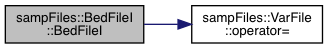
\includegraphics[width=318pt]{classsamp_files_1_1_bed_file_i_abb33c9b143ab40ee37b56a62e7e999f8_cgraph}
\end{center}
\end{figure}


\subsection{Member Function Documentation}
\mbox{\Hypertarget{classsamp_files_1_1_bed_file_i_a40dbd1c78781d4eb32f59620624bfa8a}\label{classsamp_files_1_1_bed_file_i_a40dbd1c78781d4eb32f59620624bfa8a}} 
\index{samp\+Files\+::\+Bed\+FileI@{samp\+Files\+::\+Bed\+FileI}!\+\_\+fam\+Lines@{\+\_\+fam\+Lines}}
\index{\+\_\+fam\+Lines@{\+\_\+fam\+Lines}!samp\+Files\+::\+Bed\+FileI@{samp\+Files\+::\+Bed\+FileI}}
\subsubsection{\texorpdfstring{\+\_\+fam\+Lines()}{\_famLines()}\hspace{0.1cm}{\footnotesize\ttfamily [1/2]}}
{\footnotesize\ttfamily uint64\+\_\+t Bed\+File\+I\+::\+\_\+fam\+Lines (\begin{DoxyParamCaption}{ }\end{DoxyParamCaption})\hspace{0.3cm}{\ttfamily [protected]}}



Get number of lines in the {\ttfamily \+\_\+fam\+File} 

Assumes Unix-\/like line endings. The result is equal to the number of individuals.

\begin{DoxyReturn}{Returns}
number of lines in {\ttfamily \+\_\+fam\+File} 
\end{DoxyReturn}
\mbox{\Hypertarget{classsamp_files_1_1_bed_file_i_ad0898ea2f902dbd7c01e66ae3133c0b9}\label{classsamp_files_1_1_bed_file_i_ad0898ea2f902dbd7c01e66ae3133c0b9}} 
\index{samp\+Files\+::\+Bed\+FileI@{samp\+Files\+::\+Bed\+FileI}!\+\_\+fam\+Lines@{\+\_\+fam\+Lines}}
\index{\+\_\+fam\+Lines@{\+\_\+fam\+Lines}!samp\+Files\+::\+Bed\+FileI@{samp\+Files\+::\+Bed\+FileI}}
\subsubsection{\texorpdfstring{\+\_\+fam\+Lines()}{\_famLines()}\hspace{0.1cm}{\footnotesize\ttfamily [2/2]}}
{\footnotesize\ttfamily uint64\+\_\+t Bed\+File\+I\+::\+\_\+fam\+Lines (\begin{DoxyParamCaption}\item[{fstream \&}]{fam }\end{DoxyParamCaption})\hspace{0.3cm}{\ttfamily [protected]}}



Copy the .fam file and count number of lines. 

Assumes Unix-\/like line endings. The result is equal to the number of individuals. The current object\textquotesingle{}s .fam file is copied to the provided file stream, which should be open for raading. If not, the function throws a {\itshape string} object ``\+Output .fam filestream not open\textquotesingle{}\textquotesingle{}.


\begin{DoxyParams}[1]{Parameters}
\mbox{\tt in}  & {\em fam} & .fam file stream\\
\hline
\end{DoxyParams}
\begin{DoxyReturn}{Returns}
number of lines in {\ttfamily \+\_\+fam\+File} 
\end{DoxyReturn}
\mbox{\Hypertarget{classsamp_files_1_1_bed_file_i_a9b6f8cbb9ae05056a7cd3d487fb26c30}\label{classsamp_files_1_1_bed_file_i_a9b6f8cbb9ae05056a7cd3d487fb26c30}} 
\index{samp\+Files\+::\+Bed\+FileI@{samp\+Files\+::\+Bed\+FileI}!\+\_\+ld@{\+\_\+ld}}
\index{\+\_\+ld@{\+\_\+ld}!samp\+Files\+::\+Bed\+FileI@{samp\+Files\+::\+Bed\+FileI}}
\subsubsection{\texorpdfstring{\+\_\+ld()}{\_ld()}\hspace{0.1cm}{\footnotesize\ttfamily [1/2]}}
{\footnotesize\ttfamily void Bed\+File\+I\+::\+\_\+ld (\begin{DoxyParamCaption}\item[{const char $\ast$}]{snp1,  }\item[{const char $\ast$}]{snp2,  }\item[{const size\+\_\+t \&}]{N,  }\item[{const unsigned short \&}]{pad,  }\item[{double \&}]{r\+Sq,  }\item[{double \&}]{Dprime,  }\item[{double \&}]{dcnt1,  }\item[{double \&}]{dcnt2 }\end{DoxyParamCaption})\hspace{0.3cm}{\ttfamily [protected]}}



Between-\/\+S\+NP linkage disequilibrium (LD) 

Calculates two LD statistics ( $ r^2 $ and $ D' $) between two S\+N\+Ps from a B\+ED file. Missing values are ignored. If there are fewer than three haplotypes with data present at both loci, the return values are -\/9. This value is also returned if one of the loci is monomorphic after taking out missing data at the other S\+NP. Minor (not necessarily derived) allele counts are also reported to enable downstream filtering. Note that the populations are assumed diploid and the counts are of haploid chromosomes (i.\+e. one homozygote yields count of 2).


\begin{DoxyParams}[1]{Parameters}
\mbox{\tt in}  & {\em snp1} & first S\+NP \\
\hline
\mbox{\tt in}  & {\em snp2} & second S\+NP \\
\hline
\mbox{\tt in}  & {\em N} & length of the genotype vector in bytes (four genotypes per byte) \\
\hline
\mbox{\tt in}  & {\em pad} & number of bit pairs of padding in the last byte \\
\hline
\mbox{\tt out}  & {\em r\+Sq} & the $ r^2 $ estimate \\
\hline
\mbox{\tt out}  & {\em Dprime} & the $ D' $ estimate \\
\hline
\mbox{\tt out}  & {\em dcnt1} & minor allele count at locus 1 \\
\hline
\mbox{\tt out}  & {\em dcnt2} & minor allele count at locus 2 \\
\hline
\end{DoxyParams}
\mbox{\Hypertarget{classsamp_files_1_1_bed_file_i_ac0ebb71cdebd43d1b024cfc747fd53d1}\label{classsamp_files_1_1_bed_file_i_ac0ebb71cdebd43d1b024cfc747fd53d1}} 
\index{samp\+Files\+::\+Bed\+FileI@{samp\+Files\+::\+Bed\+FileI}!\+\_\+ld@{\+\_\+ld}}
\index{\+\_\+ld@{\+\_\+ld}!samp\+Files\+::\+Bed\+FileI@{samp\+Files\+::\+Bed\+FileI}}
\subsubsection{\texorpdfstring{\+\_\+ld()}{\_ld()}\hspace{0.1cm}{\footnotesize\ttfamily [2/2]}}
{\footnotesize\ttfamily void Bed\+File\+I\+::\+\_\+ld (\begin{DoxyParamCaption}\item[{const char $\ast$}]{snp1,  }\item[{const char $\ast$}]{snp2,  }\item[{const \hyperlink{classsamp_files_1_1_pop_index}{Pop\+Index} \&}]{pop\+ID,  }\item[{vector$<$ double $>$ \&}]{r\+Sq,  }\item[{vector$<$ double $>$ \&}]{Dprime,  }\item[{vector$<$ double $>$ \&}]{dcnt1,  }\item[{vector$<$ double $>$ \&}]{dcnt2 }\end{DoxyParamCaption})\hspace{0.3cm}{\ttfamily [protected]}}



Between-\/\+S\+NP LD within populations. 

Calculates two LD statistics ( $ r^2 $ and $ D' $) between two S\+N\+Ps from a B\+ED file. Missing values are ignored. If there are fewer than three haplotypes with data present at both loci, the return values are -\/9. This value is also returned if one of the loci is monomorphic after taking out missing data at the other S\+NP. Minor (not necessarily derived) allele counts are also reported to enable downstream filtering. Note that the populations are assumed diploid and the counts are of haploid chromosomes (i.\+e. one homozygote yields count of 2). The values are calculted within each population as indicated by the {\ttfamily \hyperlink{classsamp_files_1_1_pop_index}{Pop\+Index}} object. The results are returned in the supplied vectors, which are assumed to be of correct size. Since this is an internal function unexposed to the user, this is not chaecked to save on compuation steps. Care must be taken that the {\ttfamily char} arrays passed to the function have lengths compatible with the number of individuals indexed by {\ttfamily \hyperlink{classsamp_files_1_1_pop_index}{Pop\+Index}}. This is not checked.


\begin{DoxyParams}[1]{Parameters}
\mbox{\tt in}  & {\em snp1} & first S\+NP \\
\hline
\mbox{\tt in}  & {\em snp2} & second S\+NP \\
\hline
\mbox{\tt in}  & {\em pop\+ID} & population index \\
\hline
\mbox{\tt out}  & {\em r\+Sq} & vector of $ r^2 $ estimates \\
\hline
\mbox{\tt out}  & {\em Dprime} & vector of $ D' $ estimates \\
\hline
\mbox{\tt out}  & {\em dcnt1} & vector of minor allele counts at locus 1 \\
\hline
\mbox{\tt out}  & {\em dcnt2} & vector of minor allele counts at locus 2 \\
\hline
\end{DoxyParams}
Here is the call graph for this function\+:\nopagebreak
\begin{figure}[H]
\begin{center}
\leavevmode
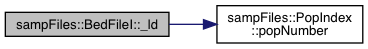
\includegraphics[width=348pt]{classsamp_files_1_1_bed_file_i_ac0ebb71cdebd43d1b024cfc747fd53d1_cgraph}
\end{center}
\end{figure}
\mbox{\Hypertarget{classsamp_files_1_1_bed_file_i_ae0a3bbe25250cb77336d1eb07643c03e}\label{classsamp_files_1_1_bed_file_i_ae0a3bbe25250cb77336d1eb07643c03e}} 
\index{samp\+Files\+::\+Bed\+FileI@{samp\+Files\+::\+Bed\+FileI}!\+\_\+num\+Lines@{\+\_\+num\+Lines}}
\index{\+\_\+num\+Lines@{\+\_\+num\+Lines}!samp\+Files\+::\+Bed\+FileI@{samp\+Files\+::\+Bed\+FileI}}
\subsubsection{\texorpdfstring{\+\_\+num\+Lines()}{\_numLines()}}
{\footnotesize\ttfamily uint64\+\_\+t Bed\+File\+I\+::\+\_\+num\+Lines (\begin{DoxyParamCaption}{ }\end{DoxyParamCaption})\hspace{0.3cm}{\ttfamily [protected]}}



Get number of lines in the {\ttfamily \+\_\+bim\+File} 

Assumes Unix-\/like line endings. The result is equal to the number of S\+N\+Ps.

\begin{DoxyReturn}{Returns}
number of lines in {\ttfamily \+\_\+bim\+File} 
\end{DoxyReturn}
\mbox{\Hypertarget{classsamp_files_1_1_bed_file_i_ac1050b3b8aec9108ae05285cbdfd85b3}\label{classsamp_files_1_1_bed_file_i_ac1050b3b8aec9108ae05285cbdfd85b3}} 
\index{samp\+Files\+::\+Bed\+FileI@{samp\+Files\+::\+Bed\+FileI}!sample@{sample}}
\index{sample@{sample}!samp\+Files\+::\+Bed\+FileI@{samp\+Files\+::\+Bed\+FileI}}
\subsubsection{\texorpdfstring{sample()}{sample()}}
{\footnotesize\ttfamily void Bed\+File\+I\+::sample (\begin{DoxyParamCaption}\item[{\hyperlink{classsamp_files_1_1_bed_file_o}{Bed\+FileO} \&}]{out,  }\item[{const uint64\+\_\+t \&}]{n }\end{DoxyParamCaption})}



Sample S\+N\+Ps and save to B\+ED file. 

Sample $n$ S\+N\+Ps without replacement from the file represented by the current object and save to the {\ttfamily out} object. Uses Vitter\textquotesingle{}s \cite{vitter87a} method. Number of samples has to be smaller that the number of S\+N\+Ps in the file.


\begin{DoxyParams}[1]{Parameters}
\mbox{\tt in}  & {\em out} & output object \\
\hline
\mbox{\tt in}  & {\em n} & number of S\+N\+Ps to sample \\
\hline
\end{DoxyParams}
Here is the call graph for this function\+:\nopagebreak
\begin{figure}[H]
\begin{center}
\leavevmode
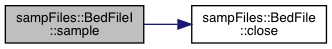
\includegraphics[width=321pt]{classsamp_files_1_1_bed_file_i_ac1050b3b8aec9108ae05285cbdfd85b3_cgraph}
\end{center}
\end{figure}
\mbox{\Hypertarget{classsamp_files_1_1_bed_file_i_ae502304386c409e9312a090a189ab694}\label{classsamp_files_1_1_bed_file_i_ae502304386c409e9312a090a189ab694}} 
\index{samp\+Files\+::\+Bed\+FileI@{samp\+Files\+::\+Bed\+FileI}!sample\+LD@{sample\+LD}}
\index{sample\+LD@{sample\+LD}!samp\+Files\+::\+Bed\+FileI@{samp\+Files\+::\+Bed\+FileI}}
\subsubsection{\texorpdfstring{sample\+L\+D()}{sampleLD()}\hspace{0.1cm}{\footnotesize\ttfamily [1/2]}}
{\footnotesize\ttfamily void Bed\+File\+I\+::sample\+LD (\begin{DoxyParamCaption}\item[{const uint64\+\_\+t \&}]{n }\end{DoxyParamCaption})}



Linkage disequilibrium among sampled sites. 

Samples sequential pairs of S\+N\+Ps and calculates two LD measures ( $ r^2 $ and $ D' $). Saves to a file with the same name as the one preceding the .bed etc extensions, but adds \+\_\+\+L\+D.\+tsv at the end. Each line is tab-\/delimited with the chromosome number (from the .bim file), between-\/\+S\+NP distance, non-\/reference allele count for each S\+NP, $ r^2 $, and $ D' $. Missing data are ignored (only pairwise-\/complete observations are included). If one of the S\+N\+Ps is monomorphic or if the total number of pairwise present genotypes is fewer than three (exclusive), the LD measures are returned as -\/9 to indicate missing values.


\begin{DoxyParams}[1]{Parameters}
\mbox{\tt in}  & {\em n} & number of S\+NP pairs to sample \\
\hline
\end{DoxyParams}
Here is the call graph for this function\+:\nopagebreak
\begin{figure}[H]
\begin{center}
\leavevmode
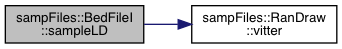
\includegraphics[width=329pt]{classsamp_files_1_1_bed_file_i_ae502304386c409e9312a090a189ab694_cgraph}
\end{center}
\end{figure}
\mbox{\Hypertarget{classsamp_files_1_1_bed_file_i_aca4f3b7ba7fa45b6a0ed1341606858f1}\label{classsamp_files_1_1_bed_file_i_aca4f3b7ba7fa45b6a0ed1341606858f1}} 
\index{samp\+Files\+::\+Bed\+FileI@{samp\+Files\+::\+Bed\+FileI}!sample\+LD@{sample\+LD}}
\index{sample\+LD@{sample\+LD}!samp\+Files\+::\+Bed\+FileI@{samp\+Files\+::\+Bed\+FileI}}
\subsubsection{\texorpdfstring{sample\+L\+D()}{sampleLD()}\hspace{0.1cm}{\footnotesize\ttfamily [2/2]}}
{\footnotesize\ttfamily void Bed\+File\+I\+::sample\+LD (\begin{DoxyParamCaption}\item[{const \hyperlink{classsamp_files_1_1_pop_index}{Pop\+Index} \&}]{pop\+ID,  }\item[{const uint64\+\_\+t \&}]{n }\end{DoxyParamCaption})}



LD among sampled sites within populations. 

Samples sequential pairs of S\+N\+Ps and calculates two LD measures ( $ r^2 $ and $ D' $) within populations indicated by {\ttfamily \hyperlink{classsamp_files_1_1_pop_index}{Pop\+Index}}. Saves to a file with the same name as the one preceding the .bed etc extensions, but adds \+\_\+\+L\+D.\+tsv at the end. Each line is tab-\/delimited with the chromosome number (from the .bim file), between-\/\+S\+NP distance, non-\/reference allele count for each S\+NP, $ r^2 $, and $ D' $. Missing data are ignored (only pairwise-\/complete observations are included). If one of the S\+N\+Ps is monomorphic or if the total number of pairwise present genotypes is fewer than three (exclusive), the LD measures are returned as -\/9 to indicate missing values.


\begin{DoxyParams}[1]{Parameters}
\mbox{\tt in}  & {\em pop\+ID} & population index \\
\hline
\mbox{\tt in}  & {\em n} & number of S\+NP pairs to sample \\
\hline
\end{DoxyParams}
Here is the call graph for this function\+:\nopagebreak
\begin{figure}[H]
\begin{center}
\leavevmode
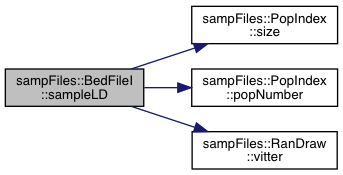
\includegraphics[width=329pt]{classsamp_files_1_1_bed_file_i_aca4f3b7ba7fa45b6a0ed1341606858f1_cgraph}
\end{center}
\end{figure}


The documentation for this class was generated from the following files\+:\begin{DoxyCompactItemize}
\item 
\hyperlink{varfiles_8hpp}{varfiles.\+hpp}\item 
\hyperlink{varfiles_8cpp}{varfiles.\+cpp}\end{DoxyCompactItemize}

\hypertarget{classsamp_files_1_1_bed_file_o}{}\section{samp\+Files\+:\+:Bed\+FileO Class Reference}
\label{classsamp_files_1_1_bed_file_o}\index{samp\+Files\+::\+Bed\+FileO@{samp\+Files\+::\+Bed\+FileO}}


B\+ED file output class.  




{\ttfamily \#include $<$varfiles.\+hpp$>$}



Inheritance diagram for samp\+Files\+:\+:Bed\+FileO\+:\nopagebreak
\begin{figure}[H]
\begin{center}
\leavevmode
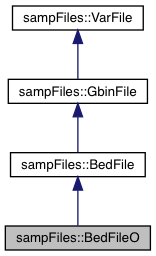
\includegraphics[width=189pt]{classsamp_files_1_1_bed_file_o__inherit__graph}
\end{center}
\end{figure}


Collaboration diagram for samp\+Files\+:\+:Bed\+FileO\+:\nopagebreak
\begin{figure}[H]
\begin{center}
\leavevmode
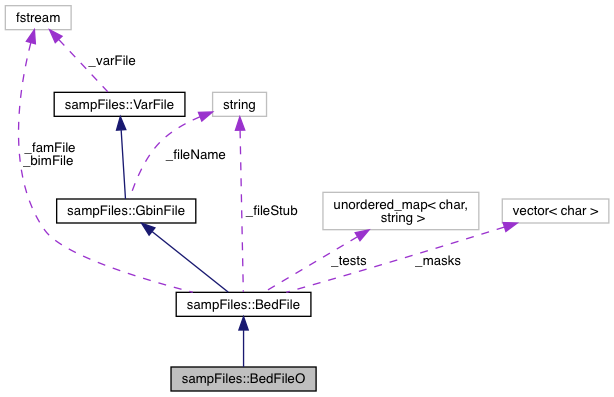
\includegraphics[width=350pt]{classsamp_files_1_1_bed_file_o__coll__graph}
\end{center}
\end{figure}
\subsection*{Public Member Functions}
\begin{DoxyCompactItemize}
\item 
\mbox{\Hypertarget{classsamp_files_1_1_bed_file_o_aebdfbb617b52a61a97591b37ccbb7f0a}\label{classsamp_files_1_1_bed_file_o_aebdfbb617b52a61a97591b37ccbb7f0a}} 
\hyperlink{classsamp_files_1_1_bed_file_o_aebdfbb617b52a61a97591b37ccbb7f0a}{Bed\+FileO} ()
\begin{DoxyCompactList}\small\item\em Default constructor. \end{DoxyCompactList}\item 
\hyperlink{classsamp_files_1_1_bed_file_o_a0abab96a74b4f8d92d85dbd147e7a9ae}{Bed\+FileO} (const string \&stub\+Name)
\begin{DoxyCompactList}\small\item\em File name constructor. \end{DoxyCompactList}\item 
\mbox{\Hypertarget{classsamp_files_1_1_bed_file_o_a68243fc4f91042a5de691c5c3ed833d4}\label{classsamp_files_1_1_bed_file_o_a68243fc4f91042a5de691c5c3ed833d4}} 
\hyperlink{classsamp_files_1_1_bed_file_o_a68243fc4f91042a5de691c5c3ed833d4}{Bed\+FileO} (const \hyperlink{classsamp_files_1_1_bed_file_o}{Bed\+FileO} \&in)=default
\begin{DoxyCompactList}\small\item\em Copy constructor. \end{DoxyCompactList}\item 
\mbox{\Hypertarget{classsamp_files_1_1_bed_file_o_a3e0239d1721dc5ae7232e248dfbd43a5}\label{classsamp_files_1_1_bed_file_o_a3e0239d1721dc5ae7232e248dfbd43a5}} 
\hyperlink{classsamp_files_1_1_bed_file_o}{Bed\+FileO} \& \hyperlink{classsamp_files_1_1_bed_file_o_a3e0239d1721dc5ae7232e248dfbd43a5}{operator=} (const \hyperlink{classsamp_files_1_1_bed_file_o}{Bed\+FileO} \&in)=default
\begin{DoxyCompactList}\small\item\em Copy assignment. \end{DoxyCompactList}\item 
\mbox{\Hypertarget{classsamp_files_1_1_bed_file_o_aa441eeb64a48884637b3004a98b5abc5}\label{classsamp_files_1_1_bed_file_o_aa441eeb64a48884637b3004a98b5abc5}} 
\hyperlink{classsamp_files_1_1_bed_file_o_aa441eeb64a48884637b3004a98b5abc5}{Bed\+FileO} (\hyperlink{classsamp_files_1_1_bed_file_o}{Bed\+FileO} \&\&in)=default
\begin{DoxyCompactList}\small\item\em Move constructor. \end{DoxyCompactList}\item 
\mbox{\Hypertarget{classsamp_files_1_1_bed_file_o_aede4f52d7769a1f6239d3b0a5d0fae40}\label{classsamp_files_1_1_bed_file_o_aede4f52d7769a1f6239d3b0a5d0fae40}} 
\hyperlink{classsamp_files_1_1_bed_file_o}{Bed\+FileO} \& \hyperlink{classsamp_files_1_1_bed_file_o_aede4f52d7769a1f6239d3b0a5d0fae40}{operator=} (\hyperlink{classsamp_files_1_1_bed_file_o}{Bed\+FileO} \&\&in)=default
\begin{DoxyCompactList}\small\item\em Move assignment. \end{DoxyCompactList}\item 
\mbox{\Hypertarget{classsamp_files_1_1_bed_file_o_a6ed06cfab3d67901384f523fe7d3f734}\label{classsamp_files_1_1_bed_file_o_a6ed06cfab3d67901384f523fe7d3f734}} 
\hyperlink{classsamp_files_1_1_bed_file_o_a6ed06cfab3d67901384f523fe7d3f734}{$\sim$\+Bed\+FileO} ()
\begin{DoxyCompactList}\small\item\em Destructor. \end{DoxyCompactList}\item 
\mbox{\Hypertarget{classsamp_files_1_1_bed_file_o_a70bee4622ebf338c6f17859f2409d17c}\label{classsamp_files_1_1_bed_file_o_a70bee4622ebf338c6f17859f2409d17c}} 
void \hyperlink{classsamp_files_1_1_bed_file_o_a70bee4622ebf338c6f17859f2409d17c}{open} ()
\begin{DoxyCompactList}\small\item\em Open stream to write. \end{DoxyCompactList}\end{DoxyCompactItemize}
\subsection*{Friends}
\begin{DoxyCompactItemize}
\item 
\mbox{\Hypertarget{classsamp_files_1_1_bed_file_o_a83903ab2cdc6179910bbb04232c007ea}\label{classsamp_files_1_1_bed_file_o_a83903ab2cdc6179910bbb04232c007ea}} 
class {\bfseries Bed\+FileI}
\end{DoxyCompactItemize}
\subsection*{Additional Inherited Members}


\subsection{Detailed Description}
B\+ED file output class. 

Writes to B\+ED files and the auxiliary files that come with them (.fam and .bim) as necessary. Data are written in the S\+N\+P-\/major format. 

\subsection{Constructor \& Destructor Documentation}
\mbox{\Hypertarget{classsamp_files_1_1_bed_file_o_a0abab96a74b4f8d92d85dbd147e7a9ae}\label{classsamp_files_1_1_bed_file_o_a0abab96a74b4f8d92d85dbd147e7a9ae}} 
\index{samp\+Files\+::\+Bed\+FileO@{samp\+Files\+::\+Bed\+FileO}!Bed\+FileO@{Bed\+FileO}}
\index{Bed\+FileO@{Bed\+FileO}!samp\+Files\+::\+Bed\+FileO@{samp\+Files\+::\+Bed\+FileO}}
\subsubsection{\texorpdfstring{Bed\+File\+O()}{BedFileO()}}
{\footnotesize\ttfamily samp\+Files\+::\+Bed\+File\+O\+::\+Bed\+FileO (\begin{DoxyParamCaption}\item[{const string \&}]{stub\+Name }\end{DoxyParamCaption})\hspace{0.3cm}{\ttfamily [inline]}}



File name constructor. 


\begin{DoxyParams}[1]{Parameters}
\mbox{\tt in}  & {\em stub\+Name} & file name minus the extension \\
\hline
\end{DoxyParams}
Here is the call graph for this function\+:\nopagebreak
\begin{figure}[H]
\begin{center}
\leavevmode
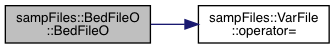
\includegraphics[width=323pt]{classsamp_files_1_1_bed_file_o_a0abab96a74b4f8d92d85dbd147e7a9ae_cgraph}
\end{center}
\end{figure}


The documentation for this class was generated from the following files\+:\begin{DoxyCompactItemize}
\item 
\hyperlink{varfiles_8hpp}{varfiles.\+hpp}\item 
\hyperlink{varfiles_8cpp}{varfiles.\+cpp}\end{DoxyCompactItemize}

\hypertarget{classsamp_files_1_1_gbin_file}{}\section{samp\+Files\+:\+:Gbin\+File Class Reference}
\label{classsamp_files_1_1_gbin_file}\index{samp\+Files\+::\+Gbin\+File@{samp\+Files\+::\+Gbin\+File}}


Generic binary file base class.  




{\ttfamily \#include $<$varfiles.\+hpp$>$}



Inheritance diagram for samp\+Files\+:\+:Gbin\+File\+:\nopagebreak
\begin{figure}[H]
\begin{center}
\leavevmode
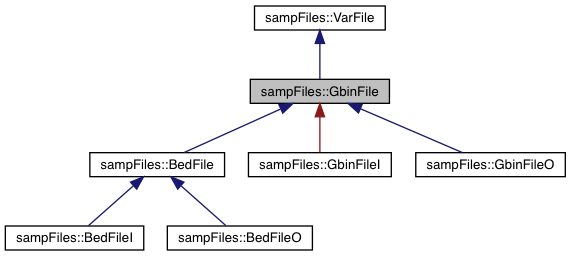
\includegraphics[width=350pt]{classsamp_files_1_1_gbin_file__inherit__graph}
\end{center}
\end{figure}


Collaboration diagram for samp\+Files\+:\+:Gbin\+File\+:\nopagebreak
\begin{figure}[H]
\begin{center}
\leavevmode
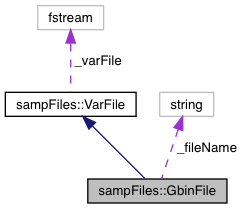
\includegraphics[width=254pt]{classsamp_files_1_1_gbin_file__coll__graph}
\end{center}
\end{figure}
\subsection*{Public Member Functions}
\begin{DoxyCompactItemize}
\item 
\mbox{\Hypertarget{classsamp_files_1_1_gbin_file_a43b61a06baecc13a76044a23d1fdd9e3}\label{classsamp_files_1_1_gbin_file_a43b61a06baecc13a76044a23d1fdd9e3}} 
\hyperlink{classsamp_files_1_1_gbin_file_a43b61a06baecc13a76044a23d1fdd9e3}{Gbin\+File} ()
\begin{DoxyCompactList}\small\item\em Default constructor. \end{DoxyCompactList}\item 
\hyperlink{classsamp_files_1_1_gbin_file_ac88b766b15e644506fa4bca84a650f3b}{Gbin\+File} (const string \&file\+Name, const size\+\_\+t \&n\+Cols, const size\+\_\+t \&elem\+Size)
\begin{DoxyCompactList}\small\item\em Constructor with file name. \end{DoxyCompactList}\item 
\mbox{\Hypertarget{classsamp_files_1_1_gbin_file_aed811f6b8b264011420bba4d957ae50a}\label{classsamp_files_1_1_gbin_file_aed811f6b8b264011420bba4d957ae50a}} 
\hyperlink{classsamp_files_1_1_gbin_file_aed811f6b8b264011420bba4d957ae50a}{Gbin\+File} (const \hyperlink{classsamp_files_1_1_gbin_file}{Gbin\+File} \&in)=default
\begin{DoxyCompactList}\small\item\em Copy constructor. \end{DoxyCompactList}\item 
\mbox{\Hypertarget{classsamp_files_1_1_gbin_file_a5a09f00116fa5a8758e7c72f069ee232}\label{classsamp_files_1_1_gbin_file_a5a09f00116fa5a8758e7c72f069ee232}} 
\hyperlink{classsamp_files_1_1_gbin_file}{Gbin\+File} \& \hyperlink{classsamp_files_1_1_gbin_file_a5a09f00116fa5a8758e7c72f069ee232}{operator=} (const \hyperlink{classsamp_files_1_1_gbin_file}{Gbin\+File} \&in)=default
\begin{DoxyCompactList}\small\item\em Copy assignment. \end{DoxyCompactList}\item 
\mbox{\Hypertarget{classsamp_files_1_1_gbin_file_a406447ac7a681982a4d2e8d71b862f2b}\label{classsamp_files_1_1_gbin_file_a406447ac7a681982a4d2e8d71b862f2b}} 
\hyperlink{classsamp_files_1_1_gbin_file_a406447ac7a681982a4d2e8d71b862f2b}{Gbin\+File} (\hyperlink{classsamp_files_1_1_gbin_file}{Gbin\+File} \&\&in)=default
\begin{DoxyCompactList}\small\item\em Move constructor. \end{DoxyCompactList}\item 
\mbox{\Hypertarget{classsamp_files_1_1_gbin_file_a8c1e649e522524a43e92086c5faa5d5e}\label{classsamp_files_1_1_gbin_file_a8c1e649e522524a43e92086c5faa5d5e}} 
\hyperlink{classsamp_files_1_1_gbin_file}{Gbin\+File} \& \hyperlink{classsamp_files_1_1_gbin_file_a8c1e649e522524a43e92086c5faa5d5e}{operator=} (\hyperlink{classsamp_files_1_1_gbin_file}{Gbin\+File} \&\&in)=default
\begin{DoxyCompactList}\small\item\em Move assignment. \end{DoxyCompactList}\item 
\mbox{\Hypertarget{classsamp_files_1_1_gbin_file_adf3cbbca2a4d63146a160b44176061bf}\label{classsamp_files_1_1_gbin_file_adf3cbbca2a4d63146a160b44176061bf}} 
\hyperlink{classsamp_files_1_1_gbin_file_adf3cbbca2a4d63146a160b44176061bf}{$\sim$\+Gbin\+File} ()
\begin{DoxyCompactList}\small\item\em Destructor. \end{DoxyCompactList}\item 
\mbox{\Hypertarget{classsamp_files_1_1_gbin_file_a1afd82548553da38e55d0b1a45dd87de}\label{classsamp_files_1_1_gbin_file_a1afd82548553da38e55d0b1a45dd87de}} 
virtual void \hyperlink{classsamp_files_1_1_gbin_file_a1afd82548553da38e55d0b1a45dd87de}{open} ()
\begin{DoxyCompactList}\small\item\em Open stream (does nothing) \end{DoxyCompactList}\item 
\mbox{\Hypertarget{classsamp_files_1_1_gbin_file_aff640b9e51117c18208444a86f2515cf}\label{classsamp_files_1_1_gbin_file_aff640b9e51117c18208444a86f2515cf}} 
virtual void \hyperlink{classsamp_files_1_1_gbin_file_aff640b9e51117c18208444a86f2515cf}{close} ()
\begin{DoxyCompactList}\small\item\em Close stream. \end{DoxyCompactList}\end{DoxyCompactItemize}
\subsection*{Protected Attributes}
\begin{DoxyCompactItemize}
\item 
\mbox{\Hypertarget{classsamp_files_1_1_gbin_file_a14d7824f305dc27e39fa62fc25af3a15}\label{classsamp_files_1_1_gbin_file_a14d7824f305dc27e39fa62fc25af3a15}} 
string \hyperlink{classsamp_files_1_1_gbin_file_a14d7824f305dc27e39fa62fc25af3a15}{\+\_\+file\+Name}
\begin{DoxyCompactList}\small\item\em File name. \end{DoxyCompactList}\item 
\mbox{\Hypertarget{classsamp_files_1_1_gbin_file_a3812c4ed2ddc7554dec1bae48905b9fe}\label{classsamp_files_1_1_gbin_file_a3812c4ed2ddc7554dec1bae48905b9fe}} 
size\+\_\+t \hyperlink{classsamp_files_1_1_gbin_file_a3812c4ed2ddc7554dec1bae48905b9fe}{\+\_\+n\+Cols}
\begin{DoxyCompactList}\small\item\em Number of elements in a row. \end{DoxyCompactList}\item 
\mbox{\Hypertarget{classsamp_files_1_1_gbin_file_ad3d585c1160916f60bde3fdd17a077ef}\label{classsamp_files_1_1_gbin_file_ad3d585c1160916f60bde3fdd17a077ef}} 
size\+\_\+t \hyperlink{classsamp_files_1_1_gbin_file_ad3d585c1160916f60bde3fdd17a077ef}{\+\_\+elem\+Size}
\begin{DoxyCompactList}\small\item\em Size of each element in bytes. \end{DoxyCompactList}\end{DoxyCompactItemize}
\subsection*{Additional Inherited Members}


\subsection{Detailed Description}
Generic binary file base class. 

Sets up streams for binary files. No support for header lines. 

\subsection{Constructor \& Destructor Documentation}
\mbox{\Hypertarget{classsamp_files_1_1_gbin_file_ac88b766b15e644506fa4bca84a650f3b}\label{classsamp_files_1_1_gbin_file_ac88b766b15e644506fa4bca84a650f3b}} 
\index{samp\+Files\+::\+Gbin\+File@{samp\+Files\+::\+Gbin\+File}!Gbin\+File@{Gbin\+File}}
\index{Gbin\+File@{Gbin\+File}!samp\+Files\+::\+Gbin\+File@{samp\+Files\+::\+Gbin\+File}}
\subsubsection{\texorpdfstring{Gbin\+File()}{GbinFile()}}
{\footnotesize\ttfamily samp\+Files\+::\+Gbin\+File\+::\+Gbin\+File (\begin{DoxyParamCaption}\item[{const string \&}]{file\+Name,  }\item[{const size\+\_\+t \&}]{n\+Cols,  }\item[{const size\+\_\+t \&}]{elem\+Size }\end{DoxyParamCaption})\hspace{0.3cm}{\ttfamily [inline]}}



Constructor with file name. 

Throws ``\+Number of elements not divisible by the number of columns\textquotesingle{}\textquotesingle{} if the total number of elements is not divisible by the number of elements in a column.


\begin{DoxyParams}[1]{Parameters}
\mbox{\tt in}  & {\em file\+Name} & file name \\
\hline
\mbox{\tt in}  & {\em n\+Cols} & number of columns, or elements in a row \\
\hline
\mbox{\tt in}  & {\em elem\+Size} & size of each element in bytes \\
\hline
\end{DoxyParams}
Here is the call graph for this function\+:\nopagebreak
\begin{figure}[H]
\begin{center}
\leavevmode
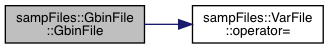
\includegraphics[width=318pt]{classsamp_files_1_1_gbin_file_ac88b766b15e644506fa4bca84a650f3b_cgraph}
\end{center}
\end{figure}


The documentation for this class was generated from the following files\+:\begin{DoxyCompactItemize}
\item 
\hyperlink{varfiles_8hpp}{varfiles.\+hpp}\item 
\hyperlink{varfiles_8cpp}{varfiles.\+cpp}\end{DoxyCompactItemize}

\hypertarget{classsamp_files_1_1_gbin_file_i}{}\section{samp\+Files\+:\+:Gbin\+FileI Class Reference}
\label{classsamp_files_1_1_gbin_file_i}\index{samp\+Files\+::\+Gbin\+FileI@{samp\+Files\+::\+Gbin\+FileI}}


Binary file input class.  




{\ttfamily \#include $<$varfiles.\+hpp$>$}



Inheritance diagram for samp\+Files\+:\+:Gbin\+FileI\+:\nopagebreak
\begin{figure}[H]
\begin{center}
\leavevmode
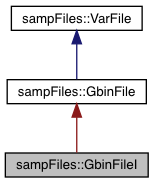
\includegraphics[width=187pt]{classsamp_files_1_1_gbin_file_i__inherit__graph}
\end{center}
\end{figure}


Collaboration diagram for samp\+Files\+:\+:Gbin\+FileI\+:\nopagebreak
\begin{figure}[H]
\begin{center}
\leavevmode
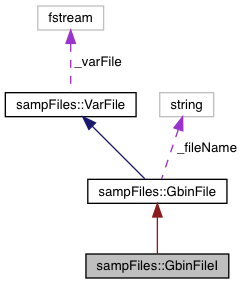
\includegraphics[width=254pt]{classsamp_files_1_1_gbin_file_i__coll__graph}
\end{center}
\end{figure}
\subsection*{Public Member Functions}
\begin{DoxyCompactItemize}
\item 
\mbox{\Hypertarget{classsamp_files_1_1_gbin_file_i_a41599498567932edd1ed3961efbb4dd7}\label{classsamp_files_1_1_gbin_file_i_a41599498567932edd1ed3961efbb4dd7}} 
\hyperlink{classsamp_files_1_1_gbin_file_i_a41599498567932edd1ed3961efbb4dd7}{Gbin\+FileI} ()
\begin{DoxyCompactList}\small\item\em Default constructor. \end{DoxyCompactList}\item 
\hyperlink{classsamp_files_1_1_gbin_file_i_ac77637d71f66c575de57443d9220984a}{Gbin\+FileI} (const string \&file\+Name, const size\+\_\+t \&n\+Cols, const size\+\_\+t \&elem\+Size)
\begin{DoxyCompactList}\small\item\em File name constructor. \end{DoxyCompactList}\item 
\mbox{\Hypertarget{classsamp_files_1_1_gbin_file_i_aa72b1178ae2bf593812e9db019362388}\label{classsamp_files_1_1_gbin_file_i_aa72b1178ae2bf593812e9db019362388}} 
\hyperlink{classsamp_files_1_1_gbin_file_i_aa72b1178ae2bf593812e9db019362388}{Gbin\+FileI} (const \hyperlink{classsamp_files_1_1_gbin_file_i}{Gbin\+FileI} \&in)=default
\begin{DoxyCompactList}\small\item\em Copy constructor. \end{DoxyCompactList}\item 
\mbox{\Hypertarget{classsamp_files_1_1_gbin_file_i_aeb231168e0b13ea71cb8382c2bfa2e5a}\label{classsamp_files_1_1_gbin_file_i_aeb231168e0b13ea71cb8382c2bfa2e5a}} 
\hyperlink{classsamp_files_1_1_gbin_file_i}{Gbin\+FileI} \& \hyperlink{classsamp_files_1_1_gbin_file_i_aeb231168e0b13ea71cb8382c2bfa2e5a}{operator=} (const \hyperlink{classsamp_files_1_1_gbin_file_i}{Gbin\+FileI} \&in)=default
\begin{DoxyCompactList}\small\item\em Copy assignment. \end{DoxyCompactList}\item 
\mbox{\Hypertarget{classsamp_files_1_1_gbin_file_i_a62f43b4cacd682e70c3ad8ae5d674d08}\label{classsamp_files_1_1_gbin_file_i_a62f43b4cacd682e70c3ad8ae5d674d08}} 
\hyperlink{classsamp_files_1_1_gbin_file_i_a62f43b4cacd682e70c3ad8ae5d674d08}{Gbin\+FileI} (\hyperlink{classsamp_files_1_1_gbin_file_i}{Gbin\+FileI} \&\&in)=default
\begin{DoxyCompactList}\small\item\em Move constructor. \end{DoxyCompactList}\item 
\mbox{\Hypertarget{classsamp_files_1_1_gbin_file_i_a7ad74147ff93849a4e5f8e5c6414a89f}\label{classsamp_files_1_1_gbin_file_i_a7ad74147ff93849a4e5f8e5c6414a89f}} 
\hyperlink{classsamp_files_1_1_gbin_file_i}{Gbin\+FileI} \& \hyperlink{classsamp_files_1_1_gbin_file_i_a7ad74147ff93849a4e5f8e5c6414a89f}{operator=} (\hyperlink{classsamp_files_1_1_gbin_file_i}{Gbin\+FileI} \&\&in)=default
\begin{DoxyCompactList}\small\item\em Move assignment. \end{DoxyCompactList}\item 
\mbox{\Hypertarget{classsamp_files_1_1_gbin_file_i_a71dcb1dfbd6fd14b7084621dbab316f6}\label{classsamp_files_1_1_gbin_file_i_a71dcb1dfbd6fd14b7084621dbab316f6}} 
\hyperlink{classsamp_files_1_1_gbin_file_i_a71dcb1dfbd6fd14b7084621dbab316f6}{$\sim$\+Gbin\+FileI} ()
\begin{DoxyCompactList}\small\item\em Destructor. \end{DoxyCompactList}\item 
\mbox{\Hypertarget{classsamp_files_1_1_gbin_file_i_af32079a08976e9343e2c9a4cb849e4e4}\label{classsamp_files_1_1_gbin_file_i_af32079a08976e9343e2c9a4cb849e4e4}} 
void \hyperlink{classsamp_files_1_1_gbin_file_i_af32079a08976e9343e2c9a4cb849e4e4}{open} ()
\begin{DoxyCompactList}\small\item\em Open stream to read. \end{DoxyCompactList}\item 
void \hyperlink{classsamp_files_1_1_gbin_file_i_ac79d132333217db28039510da20ce54e}{sample} (\hyperlink{classsamp_files_1_1_gbin_file_o}{Gbin\+FileO} \&out, const uint64\+\_\+t \&n)
\begin{DoxyCompactList}\small\item\em Sample rows and save to a binary file. \end{DoxyCompactList}\item 
\mbox{\Hypertarget{classsamp_files_1_1_gbin_file_i_a702074c0aa85213bee9f6ec19ef98de2}\label{classsamp_files_1_1_gbin_file_i_a702074c0aa85213bee9f6ec19ef98de2}} 
uint64\+\_\+t \hyperlink{classsamp_files_1_1_gbin_file_i_a702074c0aa85213bee9f6ec19ef98de2}{nlines} ()
\begin{DoxyCompactList}\small\item\em Number of rows in the object. \end{DoxyCompactList}\end{DoxyCompactItemize}
\subsection*{Protected Member Functions}
\begin{DoxyCompactItemize}
\item 
virtual uint64\+\_\+t \hyperlink{classsamp_files_1_1_gbin_file_i_a3d972257dc42d62b6c623abc591f75f0}{\+\_\+num\+Lines} ()
\begin{DoxyCompactList}\small\item\em Get number of rows in the binary file. \end{DoxyCompactList}\end{DoxyCompactItemize}


\subsection{Detailed Description}
Binary file input class. 

Reads binary files. 

\subsection{Constructor \& Destructor Documentation}
\mbox{\Hypertarget{classsamp_files_1_1_gbin_file_i_ac77637d71f66c575de57443d9220984a}\label{classsamp_files_1_1_gbin_file_i_ac77637d71f66c575de57443d9220984a}} 
\index{samp\+Files\+::\+Gbin\+FileI@{samp\+Files\+::\+Gbin\+FileI}!Gbin\+FileI@{Gbin\+FileI}}
\index{Gbin\+FileI@{Gbin\+FileI}!samp\+Files\+::\+Gbin\+FileI@{samp\+Files\+::\+Gbin\+FileI}}
\subsubsection{\texorpdfstring{Gbin\+File\+I()}{GbinFileI()}}
{\footnotesize\ttfamily samp\+Files\+::\+Gbin\+File\+I\+::\+Gbin\+FileI (\begin{DoxyParamCaption}\item[{const string \&}]{file\+Name,  }\item[{const size\+\_\+t \&}]{n\+Cols,  }\item[{const size\+\_\+t \&}]{elem\+Size }\end{DoxyParamCaption})\hspace{0.3cm}{\ttfamily [inline]}}



File name constructor. 


\begin{DoxyParams}[1]{Parameters}
\mbox{\tt in}  & {\em file\+Name} & file name including extension \\
\hline
\mbox{\tt in}  & {\em n\+Cols} & number of columns, or elements in a row \\
\hline
\mbox{\tt in}  & {\em elem\+Size} & size of each element in bytes \\
\hline
\end{DoxyParams}
Here is the call graph for this function\+:\nopagebreak
\begin{figure}[H]
\begin{center}
\leavevmode
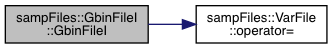
\includegraphics[width=321pt]{classsamp_files_1_1_gbin_file_i_ac77637d71f66c575de57443d9220984a_cgraph}
\end{center}
\end{figure}


\subsection{Member Function Documentation}
\mbox{\Hypertarget{classsamp_files_1_1_gbin_file_i_a3d972257dc42d62b6c623abc591f75f0}\label{classsamp_files_1_1_gbin_file_i_a3d972257dc42d62b6c623abc591f75f0}} 
\index{samp\+Files\+::\+Gbin\+FileI@{samp\+Files\+::\+Gbin\+FileI}!\+\_\+num\+Lines@{\+\_\+num\+Lines}}
\index{\+\_\+num\+Lines@{\+\_\+num\+Lines}!samp\+Files\+::\+Gbin\+FileI@{samp\+Files\+::\+Gbin\+FileI}}
\subsubsection{\texorpdfstring{\+\_\+num\+Lines()}{\_numLines()}}
{\footnotesize\ttfamily uint64\+\_\+t Gbin\+File\+I\+::\+\_\+num\+Lines (\begin{DoxyParamCaption}{ }\end{DoxyParamCaption})\hspace{0.3cm}{\ttfamily [protected]}, {\ttfamily [virtual]}}



Get number of rows in the binary file. 

Requires knowledge of the number of elements in a row and their size in bytes. Throws a {\itshape string} object ``\+Number of elements not divisible by row size\textquotesingle{}\textquotesingle{} if the total number of elements in the file is not divisible by the product of the number of columns and element size.

\begin{DoxyReturn}{Returns}
number of rows 
\end{DoxyReturn}
Here is the caller graph for this function\+:\nopagebreak
\begin{figure}[H]
\begin{center}
\leavevmode
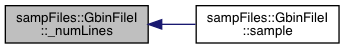
\includegraphics[width=330pt]{classsamp_files_1_1_gbin_file_i_a3d972257dc42d62b6c623abc591f75f0_icgraph}
\end{center}
\end{figure}
\mbox{\Hypertarget{classsamp_files_1_1_gbin_file_i_ac79d132333217db28039510da20ce54e}\label{classsamp_files_1_1_gbin_file_i_ac79d132333217db28039510da20ce54e}} 
\index{samp\+Files\+::\+Gbin\+FileI@{samp\+Files\+::\+Gbin\+FileI}!sample@{sample}}
\index{sample@{sample}!samp\+Files\+::\+Gbin\+FileI@{samp\+Files\+::\+Gbin\+FileI}}
\subsubsection{\texorpdfstring{sample()}{sample()}}
{\footnotesize\ttfamily void Gbin\+File\+I\+::sample (\begin{DoxyParamCaption}\item[{\hyperlink{classsamp_files_1_1_gbin_file_o}{Gbin\+FileO} \&}]{out,  }\item[{const uint64\+\_\+t \&}]{n }\end{DoxyParamCaption})}



Sample rows and save to a binary file. 

Sample $n$ lines without replacement from the file represented by the current object and save to the {\ttfamily out} object. Uses Vitter\textquotesingle{}s \cite{vitter87a} method. Number of samples has to be smaller that the number of rows in the file.


\begin{DoxyParams}[1]{Parameters}
\mbox{\tt in}  & {\em out} & output object \\
\hline
\mbox{\tt in}  & {\em n} & number of rows to sample \\
\hline
\end{DoxyParams}
Here is the call graph for this function\+:\nopagebreak
\begin{figure}[H]
\begin{center}
\leavevmode
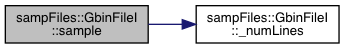
\includegraphics[width=330pt]{classsamp_files_1_1_gbin_file_i_ac79d132333217db28039510da20ce54e_cgraph}
\end{center}
\end{figure}


The documentation for this class was generated from the following files\+:\begin{DoxyCompactItemize}
\item 
\hyperlink{varfiles_8hpp}{varfiles.\+hpp}\item 
\hyperlink{varfiles_8cpp}{varfiles.\+cpp}\end{DoxyCompactItemize}

\hypertarget{classsamp_files_1_1_gbin_file_o}{}\section{samp\+Files\+:\+:Gbin\+FileO Class Reference}
\label{classsamp_files_1_1_gbin_file_o}\index{samp\+Files\+::\+Gbin\+FileO@{samp\+Files\+::\+Gbin\+FileO}}


Generic binary file output class.  




{\ttfamily \#include $<$varfiles.\+hpp$>$}



Inheritance diagram for samp\+Files\+:\+:Gbin\+FileO\+:\nopagebreak
\begin{figure}[H]
\begin{center}
\leavevmode
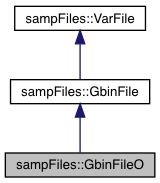
\includegraphics[width=192pt]{classsamp_files_1_1_gbin_file_o__inherit__graph}
\end{center}
\end{figure}


Collaboration diagram for samp\+Files\+:\+:Gbin\+FileO\+:\nopagebreak
\begin{figure}[H]
\begin{center}
\leavevmode
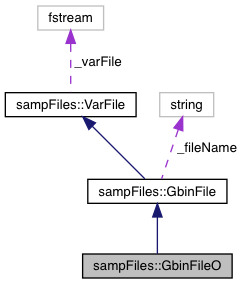
\includegraphics[width=254pt]{classsamp_files_1_1_gbin_file_o__coll__graph}
\end{center}
\end{figure}
\subsection*{Public Member Functions}
\begin{DoxyCompactItemize}
\item 
\mbox{\Hypertarget{classsamp_files_1_1_gbin_file_o_a4decba138fcab28c38f3bc342a82391c}\label{classsamp_files_1_1_gbin_file_o_a4decba138fcab28c38f3bc342a82391c}} 
\hyperlink{classsamp_files_1_1_gbin_file_o_a4decba138fcab28c38f3bc342a82391c}{Gbin\+FileO} ()
\begin{DoxyCompactList}\small\item\em Default constructor. \end{DoxyCompactList}\item 
\hyperlink{classsamp_files_1_1_gbin_file_o_a3e3315ac7b1fe5e3a8f78f06e551e855}{Gbin\+FileO} (const string \&file\+Name, const size\+\_\+t \&n\+Cols, const size\+\_\+t \&elem\+Size)
\begin{DoxyCompactList}\small\item\em File name constructor. \end{DoxyCompactList}\item 
\mbox{\Hypertarget{classsamp_files_1_1_gbin_file_o_aeaa76ff0be865d323a8f270866f854ad}\label{classsamp_files_1_1_gbin_file_o_aeaa76ff0be865d323a8f270866f854ad}} 
\hyperlink{classsamp_files_1_1_gbin_file_o_aeaa76ff0be865d323a8f270866f854ad}{Gbin\+FileO} (const \hyperlink{classsamp_files_1_1_gbin_file_o}{Gbin\+FileO} \&in)=default
\begin{DoxyCompactList}\small\item\em Copy constructor. \end{DoxyCompactList}\item 
\mbox{\Hypertarget{classsamp_files_1_1_gbin_file_o_a9ea3272eb7905b981d80c71d6c8c057c}\label{classsamp_files_1_1_gbin_file_o_a9ea3272eb7905b981d80c71d6c8c057c}} 
\hyperlink{classsamp_files_1_1_gbin_file_o}{Gbin\+FileO} \& \hyperlink{classsamp_files_1_1_gbin_file_o_a9ea3272eb7905b981d80c71d6c8c057c}{operator=} (const \hyperlink{classsamp_files_1_1_gbin_file_o}{Gbin\+FileO} \&in)=default
\begin{DoxyCompactList}\small\item\em Copy assignment. \end{DoxyCompactList}\item 
\mbox{\Hypertarget{classsamp_files_1_1_gbin_file_o_a01ffd02d1ed7fd456bf3168e26f7ba3f}\label{classsamp_files_1_1_gbin_file_o_a01ffd02d1ed7fd456bf3168e26f7ba3f}} 
\hyperlink{classsamp_files_1_1_gbin_file_o_a01ffd02d1ed7fd456bf3168e26f7ba3f}{Gbin\+FileO} (\hyperlink{classsamp_files_1_1_gbin_file_o}{Gbin\+FileO} \&\&in)=default
\begin{DoxyCompactList}\small\item\em Move constructor. \end{DoxyCompactList}\item 
\mbox{\Hypertarget{classsamp_files_1_1_gbin_file_o_a99f00b2164156c1427a91c3bcbc64605}\label{classsamp_files_1_1_gbin_file_o_a99f00b2164156c1427a91c3bcbc64605}} 
\hyperlink{classsamp_files_1_1_gbin_file_o}{Gbin\+FileO} \& \hyperlink{classsamp_files_1_1_gbin_file_o_a99f00b2164156c1427a91c3bcbc64605}{operator=} (\hyperlink{classsamp_files_1_1_gbin_file_o}{Gbin\+FileO} \&\&in)=default
\begin{DoxyCompactList}\small\item\em Move assignment. \end{DoxyCompactList}\item 
\mbox{\Hypertarget{classsamp_files_1_1_gbin_file_o_adaeea3215e02bbc94cd1ce71d47af95a}\label{classsamp_files_1_1_gbin_file_o_adaeea3215e02bbc94cd1ce71d47af95a}} 
\hyperlink{classsamp_files_1_1_gbin_file_o_adaeea3215e02bbc94cd1ce71d47af95a}{$\sim$\+Gbin\+FileO} ()
\begin{DoxyCompactList}\small\item\em Destructor. \end{DoxyCompactList}\item 
\mbox{\Hypertarget{classsamp_files_1_1_gbin_file_o_a9970e6174a76074e1c634baf58b1e6db}\label{classsamp_files_1_1_gbin_file_o_a9970e6174a76074e1c634baf58b1e6db}} 
void \hyperlink{classsamp_files_1_1_gbin_file_o_a9970e6174a76074e1c634baf58b1e6db}{open} ()
\begin{DoxyCompactList}\small\item\em Open stream to write. \end{DoxyCompactList}\end{DoxyCompactItemize}
\subsection*{Friends}
\begin{DoxyCompactItemize}
\item 
\mbox{\Hypertarget{classsamp_files_1_1_gbin_file_o_a956102d1fcb7924e5b783942f6cc023c}\label{classsamp_files_1_1_gbin_file_o_a956102d1fcb7924e5b783942f6cc023c}} 
class {\bfseries Gbin\+FileI}
\end{DoxyCompactItemize}
\subsection*{Additional Inherited Members}


\subsection{Detailed Description}
Generic binary file output class. 

Writes binary files. 

\subsection{Constructor \& Destructor Documentation}
\mbox{\Hypertarget{classsamp_files_1_1_gbin_file_o_a3e3315ac7b1fe5e3a8f78f06e551e855}\label{classsamp_files_1_1_gbin_file_o_a3e3315ac7b1fe5e3a8f78f06e551e855}} 
\index{samp\+Files\+::\+Gbin\+FileO@{samp\+Files\+::\+Gbin\+FileO}!Gbin\+FileO@{Gbin\+FileO}}
\index{Gbin\+FileO@{Gbin\+FileO}!samp\+Files\+::\+Gbin\+FileO@{samp\+Files\+::\+Gbin\+FileO}}
\subsubsection{\texorpdfstring{Gbin\+File\+O()}{GbinFileO()}}
{\footnotesize\ttfamily samp\+Files\+::\+Gbin\+File\+O\+::\+Gbin\+FileO (\begin{DoxyParamCaption}\item[{const string \&}]{file\+Name,  }\item[{const size\+\_\+t \&}]{n\+Cols,  }\item[{const size\+\_\+t \&}]{elem\+Size }\end{DoxyParamCaption})\hspace{0.3cm}{\ttfamily [inline]}}



File name constructor. 


\begin{DoxyParams}[1]{Parameters}
\mbox{\tt in}  & {\em file\+Name} & file name including extension \\
\hline
\mbox{\tt in}  & {\em n\+Cols} & number of columns, or elements in a row \\
\hline
\mbox{\tt in}  & {\em elem\+Size} & size of each element in bytes \\
\hline
\end{DoxyParams}
Here is the call graph for this function\+:\nopagebreak
\begin{figure}[H]
\begin{center}
\leavevmode
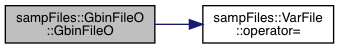
\includegraphics[width=326pt]{classsamp_files_1_1_gbin_file_o_a3e3315ac7b1fe5e3a8f78f06e551e855_cgraph}
\end{center}
\end{figure}


The documentation for this class was generated from the following files\+:\begin{DoxyCompactItemize}
\item 
\hyperlink{varfiles_8hpp}{varfiles.\+hpp}\item 
\hyperlink{varfiles_8cpp}{varfiles.\+cpp}\end{DoxyCompactItemize}

\hypertarget{classsamp_files_1_1_generate}{}\section{samp\+Files\+:\+:Generate Class Reference}
\label{classsamp_files_1_1_generate}\index{samp\+Files\+::\+Generate@{samp\+Files\+::\+Generate}}


Abstract base random number class.  




{\ttfamily \#include $<$random.\+hpp$>$}



Inheritance diagram for samp\+Files\+:\+:Generate\+:\nopagebreak
\begin{figure}[H]
\begin{center}
\leavevmode
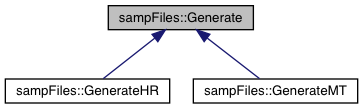
\includegraphics[width=344pt]{classsamp_files_1_1_generate__inherit__graph}
\end{center}
\end{figure}
\subsection*{Public Member Functions}
\begin{DoxyCompactItemize}
\item 
\mbox{\Hypertarget{classsamp_files_1_1_generate_af3b922c99cbfafe9d27a0ceafb87243c}\label{classsamp_files_1_1_generate_af3b922c99cbfafe9d27a0ceafb87243c}} 
virtual \hyperlink{classsamp_files_1_1_generate_af3b922c99cbfafe9d27a0ceafb87243c}{$\sim$\+Generate} ()
\begin{DoxyCompactList}\small\item\em Protected destructor. \end{DoxyCompactList}\item 
virtual volatile uint64\+\_\+t \hyperlink{classsamp_files_1_1_generate_a86fe4e68cc0809d4d936615fc60c125e}{ran\+Int} ()=0
\begin{DoxyCompactList}\small\item\em \hyperlink{classsamp_files_1_1_generate}{Generate} a (pseudo-\/)random 64-\/bit unsigned integer. \end{DoxyCompactList}\end{DoxyCompactItemize}
\subsection*{Protected Member Functions}
\begin{DoxyCompactItemize}
\item 
\mbox{\Hypertarget{classsamp_files_1_1_generate_a3096583c518c65c4e7cf1c76165fef99}\label{classsamp_files_1_1_generate_a3096583c518c65c4e7cf1c76165fef99}} 
\hyperlink{classsamp_files_1_1_generate_a3096583c518c65c4e7cf1c76165fef99}{Generate} ()
\begin{DoxyCompactList}\small\item\em Protected default constructor. \end{DoxyCompactList}\item 
\hyperlink{classsamp_files_1_1_generate_a3b9ea63228daca88614be36e796ffea1}{Generate} (const \hyperlink{classsamp_files_1_1_generate}{Generate} \&old)
\begin{DoxyCompactList}\small\item\em Protected copy constructor. \end{DoxyCompactList}\item 
\hyperlink{classsamp_files_1_1_generate_a12165e2b614b013d5eba3a893d298cea}{Generate} (\hyperlink{classsamp_files_1_1_generate}{Generate} \&\&old)
\begin{DoxyCompactList}\small\item\em Protected move constructor. \end{DoxyCompactList}\item 
\hyperlink{classsamp_files_1_1_generate}{Generate} \& \hyperlink{classsamp_files_1_1_generate_ab54ff8f5a2c497ce98a31833e2d43d66}{operator=} (const \hyperlink{classsamp_files_1_1_generate}{Generate} \&old)=default
\begin{DoxyCompactList}\small\item\em Protected copy assignment operator. \end{DoxyCompactList}\item 
\hyperlink{classsamp_files_1_1_generate}{Generate} \& \hyperlink{classsamp_files_1_1_generate_a7b7e395a2d6fe5235fe72f7bbc50e2a6}{operator=} (\hyperlink{classsamp_files_1_1_generate}{Generate} \&\&old)=default
\begin{DoxyCompactList}\small\item\em Protected move assignment. \end{DoxyCompactList}\end{DoxyCompactItemize}


\subsection{Detailed Description}
Abstract base random number class. 

Provides the interface for random or pseudorandom (depending on derived class) generation. For internal use by the {\ttfamily \hyperlink{classsamp_files_1_1_ran_draw}{Ran\+Draw}} interface class. 

\subsection{Constructor \& Destructor Documentation}
\mbox{\Hypertarget{classsamp_files_1_1_generate_a3b9ea63228daca88614be36e796ffea1}\label{classsamp_files_1_1_generate_a3b9ea63228daca88614be36e796ffea1}} 
\index{samp\+Files\+::\+Generate@{samp\+Files\+::\+Generate}!Generate@{Generate}}
\index{Generate@{Generate}!samp\+Files\+::\+Generate@{samp\+Files\+::\+Generate}}
\subsubsection{\texorpdfstring{Generate()}{Generate()}\hspace{0.1cm}{\footnotesize\ttfamily [1/2]}}
{\footnotesize\ttfamily samp\+Files\+::\+Generate\+::\+Generate (\begin{DoxyParamCaption}\item[{const \hyperlink{classsamp_files_1_1_generate}{Generate} \&}]{old }\end{DoxyParamCaption})\hspace{0.3cm}{\ttfamily [inline]}, {\ttfamily [protected]}}



Protected copy constructor. 


\begin{DoxyParams}[1]{Parameters}
\mbox{\tt in}  & {\em old} & object to copy \\
\hline
\end{DoxyParams}
\mbox{\Hypertarget{classsamp_files_1_1_generate_a12165e2b614b013d5eba3a893d298cea}\label{classsamp_files_1_1_generate_a12165e2b614b013d5eba3a893d298cea}} 
\index{samp\+Files\+::\+Generate@{samp\+Files\+::\+Generate}!Generate@{Generate}}
\index{Generate@{Generate}!samp\+Files\+::\+Generate@{samp\+Files\+::\+Generate}}
\subsubsection{\texorpdfstring{Generate()}{Generate()}\hspace{0.1cm}{\footnotesize\ttfamily [2/2]}}
{\footnotesize\ttfamily samp\+Files\+::\+Generate\+::\+Generate (\begin{DoxyParamCaption}\item[{\hyperlink{classsamp_files_1_1_generate}{Generate} \&\&}]{old }\end{DoxyParamCaption})\hspace{0.3cm}{\ttfamily [inline]}, {\ttfamily [protected]}}



Protected move constructor. 


\begin{DoxyParams}[1]{Parameters}
\mbox{\tt in}  & {\em old} & object to move \\
\hline
\end{DoxyParams}
Here is the call graph for this function\+:\nopagebreak
\begin{figure}[H]
\begin{center}
\leavevmode
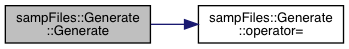
\includegraphics[width=334pt]{classsamp_files_1_1_generate_a12165e2b614b013d5eba3a893d298cea_cgraph}
\end{center}
\end{figure}


\subsection{Member Function Documentation}
\mbox{\Hypertarget{classsamp_files_1_1_generate_ab54ff8f5a2c497ce98a31833e2d43d66}\label{classsamp_files_1_1_generate_ab54ff8f5a2c497ce98a31833e2d43d66}} 
\index{samp\+Files\+::\+Generate@{samp\+Files\+::\+Generate}!operator=@{operator=}}
\index{operator=@{operator=}!samp\+Files\+::\+Generate@{samp\+Files\+::\+Generate}}
\subsubsection{\texorpdfstring{operator=()}{operator=()}\hspace{0.1cm}{\footnotesize\ttfamily [1/2]}}
{\footnotesize\ttfamily \hyperlink{classsamp_files_1_1_generate}{Generate}\& samp\+Files\+::\+Generate\+::operator= (\begin{DoxyParamCaption}\item[{const \hyperlink{classsamp_files_1_1_generate}{Generate} \&}]{old }\end{DoxyParamCaption})\hspace{0.3cm}{\ttfamily [protected]}, {\ttfamily [default]}}



Protected copy assignment operator. 


\begin{DoxyParams}[1]{Parameters}
\mbox{\tt in}  & {\em old} & object to copy \\
\hline
\end{DoxyParams}
Here is the caller graph for this function\+:\nopagebreak
\begin{figure}[H]
\begin{center}
\leavevmode
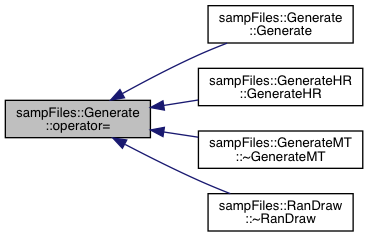
\includegraphics[width=348pt]{classsamp_files_1_1_generate_ab54ff8f5a2c497ce98a31833e2d43d66_icgraph}
\end{center}
\end{figure}
\mbox{\Hypertarget{classsamp_files_1_1_generate_a7b7e395a2d6fe5235fe72f7bbc50e2a6}\label{classsamp_files_1_1_generate_a7b7e395a2d6fe5235fe72f7bbc50e2a6}} 
\index{samp\+Files\+::\+Generate@{samp\+Files\+::\+Generate}!operator=@{operator=}}
\index{operator=@{operator=}!samp\+Files\+::\+Generate@{samp\+Files\+::\+Generate}}
\subsubsection{\texorpdfstring{operator=()}{operator=()}\hspace{0.1cm}{\footnotesize\ttfamily [2/2]}}
{\footnotesize\ttfamily \hyperlink{classsamp_files_1_1_generate}{Generate}\& samp\+Files\+::\+Generate\+::operator= (\begin{DoxyParamCaption}\item[{\hyperlink{classsamp_files_1_1_generate}{Generate} \&\&}]{old }\end{DoxyParamCaption})\hspace{0.3cm}{\ttfamily [protected]}, {\ttfamily [default]}}



Protected move assignment. 


\begin{DoxyParams}[1]{Parameters}
\mbox{\tt in}  & {\em old} & object to move \\
\hline
\end{DoxyParams}
\mbox{\Hypertarget{classsamp_files_1_1_generate_a86fe4e68cc0809d4d936615fc60c125e}\label{classsamp_files_1_1_generate_a86fe4e68cc0809d4d936615fc60c125e}} 
\index{samp\+Files\+::\+Generate@{samp\+Files\+::\+Generate}!ran\+Int@{ran\+Int}}
\index{ran\+Int@{ran\+Int}!samp\+Files\+::\+Generate@{samp\+Files\+::\+Generate}}
\subsubsection{\texorpdfstring{ran\+Int()}{ranInt()}}
{\footnotesize\ttfamily virtual volatile uint64\+\_\+t samp\+Files\+::\+Generate\+::ran\+Int (\begin{DoxyParamCaption}{ }\end{DoxyParamCaption})\hspace{0.3cm}{\ttfamily [pure virtual]}}



\hyperlink{classsamp_files_1_1_generate}{Generate} a (pseudo-\/)random 64-\/bit unsigned integer. 

\begin{DoxyReturn}{Returns}
random or pseudo-\/random 64-\/bit unsigned integer 
\end{DoxyReturn}


Implemented in \hyperlink{classsamp_files_1_1_generate_m_t_a500e163265b6fdae0a30fdacc1c37f80}{samp\+Files\+::\+Generate\+MT}, and \hyperlink{classsamp_files_1_1_generate_h_r_ac0c560c9ea17bc67470124040e0bd796}{samp\+Files\+::\+Generate\+HR}.

Here is the caller graph for this function\+:\nopagebreak
\begin{figure}[H]
\begin{center}
\leavevmode
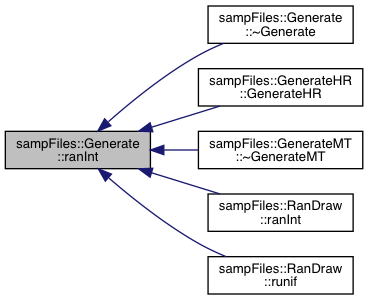
\includegraphics[width=348pt]{classsamp_files_1_1_generate_a86fe4e68cc0809d4d936615fc60c125e_icgraph}
\end{center}
\end{figure}


The documentation for this class was generated from the following file\+:\begin{DoxyCompactItemize}
\item 
\hyperlink{random_8hpp}{random.\+hpp}\end{DoxyCompactItemize}

\hypertarget{classsamp_files_1_1_generate_h_r}{}\section{samp\+Files\+:\+:Generate\+HR Class Reference}
\label{classsamp_files_1_1_generate_h_r}\index{samp\+Files\+::\+Generate\+HR@{samp\+Files\+::\+Generate\+HR}}


Hardware random number generating class.  




{\ttfamily \#include $<$random.\+hpp$>$}



Inheritance diagram for samp\+Files\+:\+:Generate\+HR\+:\nopagebreak
\begin{figure}[H]
\begin{center}
\leavevmode
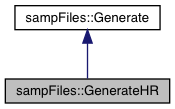
\includegraphics[width=203pt]{classsamp_files_1_1_generate_h_r__inherit__graph}
\end{center}
\end{figure}


Collaboration diagram for samp\+Files\+:\+:Generate\+HR\+:\nopagebreak
\begin{figure}[H]
\begin{center}
\leavevmode
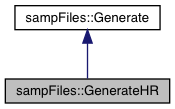
\includegraphics[width=203pt]{classsamp_files_1_1_generate_h_r__coll__graph}
\end{center}
\end{figure}
\subsection*{Public Member Functions}
\begin{DoxyCompactItemize}
\item 
\mbox{\Hypertarget{classsamp_files_1_1_generate_h_r_a2b8e7405afb964ecfbb9c005b8afbf5f}\label{classsamp_files_1_1_generate_h_r_a2b8e7405afb964ecfbb9c005b8afbf5f}} 
\hyperlink{classsamp_files_1_1_generate_h_r_a2b8e7405afb964ecfbb9c005b8afbf5f}{Generate\+HR} ()
\begin{DoxyCompactList}\small\item\em Default constructor. \end{DoxyCompactList}\item 
\mbox{\Hypertarget{classsamp_files_1_1_generate_h_r_ad275775b4118f5147d200aed1d5cc48f}\label{classsamp_files_1_1_generate_h_r_ad275775b4118f5147d200aed1d5cc48f}} 
\hyperlink{classsamp_files_1_1_generate_h_r_ad275775b4118f5147d200aed1d5cc48f}{$\sim$\+Generate\+HR} ()
\begin{DoxyCompactList}\small\item\em Destructor. \end{DoxyCompactList}\item 
\hyperlink{classsamp_files_1_1_generate_h_r_aae078758c8b83665628601feb63d956a}{Generate\+HR} (const \hyperlink{classsamp_files_1_1_generate_h_r}{Generate\+HR} \&old)
\begin{DoxyCompactList}\small\item\em Copy constructor. \end{DoxyCompactList}\item 
\hyperlink{classsamp_files_1_1_generate_h_r_adcda1d80769593770720f503e2be87ae}{Generate\+HR} (\hyperlink{classsamp_files_1_1_generate_h_r}{Generate\+HR} \&\&old)
\begin{DoxyCompactList}\small\item\em Move constructor. \end{DoxyCompactList}\item 
\hyperlink{classsamp_files_1_1_generate_h_r}{Generate\+HR} \& \hyperlink{classsamp_files_1_1_generate_h_r_a53cdc064c4d6ba7f1189948376f8b071}{operator=} (const \hyperlink{classsamp_files_1_1_generate_h_r}{Generate\+HR} \&old)=default
\begin{DoxyCompactList}\small\item\em Copy assignment operator. \end{DoxyCompactList}\item 
\hyperlink{classsamp_files_1_1_generate_h_r}{Generate\+HR} \& \hyperlink{classsamp_files_1_1_generate_h_r_aa415dd128cd0de2e567e86cb375bc919}{operator=} (\hyperlink{classsamp_files_1_1_generate_h_r}{Generate\+HR} \&\&old)=default
\begin{DoxyCompactList}\small\item\em Move assignment. \end{DoxyCompactList}\item 
volatile uint64\+\_\+t \hyperlink{classsamp_files_1_1_generate_h_r_ac0c560c9ea17bc67470124040e0bd796}{ran\+Int} ()
\begin{DoxyCompactList}\small\item\em \hyperlink{classsamp_files_1_1_generate}{Generate} a random 64-\/bit unsigned integer. \end{DoxyCompactList}\end{DoxyCompactItemize}
\subsection*{Additional Inherited Members}


\subsection{Detailed Description}
Hardware random number generating class. 

Generates random deviates from a number of distributions, using hardware random numbers ({\itshape R\+D\+R\+A\+ND} processor instruction). Health of the R\+D\+R\+A\+ND generator is tested every time a new number is required. Throws a {\ttfamily string} object \char`\"{}\+R\+D\+R\+A\+N\+D\+\_\+failed\char`\"{} if the test fails. The implementation of random 64-\/bit integer generation follows \href{https://software.intel.com/en-us/articles/intel-digital-random-number-generator-drng-software-implementation-guide}{\tt Intel\textquotesingle{}s suggestions}. 

\subsection{Constructor \& Destructor Documentation}
\mbox{\Hypertarget{classsamp_files_1_1_generate_h_r_aae078758c8b83665628601feb63d956a}\label{classsamp_files_1_1_generate_h_r_aae078758c8b83665628601feb63d956a}} 
\index{samp\+Files\+::\+Generate\+HR@{samp\+Files\+::\+Generate\+HR}!Generate\+HR@{Generate\+HR}}
\index{Generate\+HR@{Generate\+HR}!samp\+Files\+::\+Generate\+HR@{samp\+Files\+::\+Generate\+HR}}
\subsubsection{\texorpdfstring{Generate\+H\+R()}{GenerateHR()}\hspace{0.1cm}{\footnotesize\ttfamily [1/2]}}
{\footnotesize\ttfamily samp\+Files\+::\+Generate\+H\+R\+::\+Generate\+HR (\begin{DoxyParamCaption}\item[{const \hyperlink{classsamp_files_1_1_generate_h_r}{Generate\+HR} \&}]{old }\end{DoxyParamCaption})\hspace{0.3cm}{\ttfamily [inline]}}



Copy constructor. 


\begin{DoxyParams}[1]{Parameters}
\mbox{\tt in}  & {\em old} & object to copy \\
\hline
\end{DoxyParams}
\mbox{\Hypertarget{classsamp_files_1_1_generate_h_r_adcda1d80769593770720f503e2be87ae}\label{classsamp_files_1_1_generate_h_r_adcda1d80769593770720f503e2be87ae}} 
\index{samp\+Files\+::\+Generate\+HR@{samp\+Files\+::\+Generate\+HR}!Generate\+HR@{Generate\+HR}}
\index{Generate\+HR@{Generate\+HR}!samp\+Files\+::\+Generate\+HR@{samp\+Files\+::\+Generate\+HR}}
\subsubsection{\texorpdfstring{Generate\+H\+R()}{GenerateHR()}\hspace{0.1cm}{\footnotesize\ttfamily [2/2]}}
{\footnotesize\ttfamily samp\+Files\+::\+Generate\+H\+R\+::\+Generate\+HR (\begin{DoxyParamCaption}\item[{\hyperlink{classsamp_files_1_1_generate_h_r}{Generate\+HR} \&\&}]{old }\end{DoxyParamCaption})\hspace{0.3cm}{\ttfamily [inline]}}



Move constructor. 


\begin{DoxyParams}[1]{Parameters}
\mbox{\tt in}  & {\em old} & object to move \\
\hline
\end{DoxyParams}
Here is the call graph for this function\+:\nopagebreak
\begin{figure}[H]
\begin{center}
\leavevmode
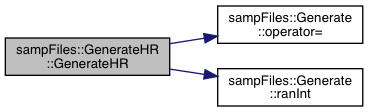
\includegraphics[width=348pt]{classsamp_files_1_1_generate_h_r_adcda1d80769593770720f503e2be87ae_cgraph}
\end{center}
\end{figure}


\subsection{Member Function Documentation}
\mbox{\Hypertarget{classsamp_files_1_1_generate_h_r_a53cdc064c4d6ba7f1189948376f8b071}\label{classsamp_files_1_1_generate_h_r_a53cdc064c4d6ba7f1189948376f8b071}} 
\index{samp\+Files\+::\+Generate\+HR@{samp\+Files\+::\+Generate\+HR}!operator=@{operator=}}
\index{operator=@{operator=}!samp\+Files\+::\+Generate\+HR@{samp\+Files\+::\+Generate\+HR}}
\subsubsection{\texorpdfstring{operator=()}{operator=()}\hspace{0.1cm}{\footnotesize\ttfamily [1/2]}}
{\footnotesize\ttfamily \hyperlink{classsamp_files_1_1_generate_h_r}{Generate\+HR}\& samp\+Files\+::\+Generate\+H\+R\+::operator= (\begin{DoxyParamCaption}\item[{const \hyperlink{classsamp_files_1_1_generate_h_r}{Generate\+HR} \&}]{old }\end{DoxyParamCaption})\hspace{0.3cm}{\ttfamily [default]}}



Copy assignment operator. 


\begin{DoxyParams}[1]{Parameters}
\mbox{\tt in}  & {\em old} & object to copy \\
\hline
\end{DoxyParams}
\mbox{\Hypertarget{classsamp_files_1_1_generate_h_r_aa415dd128cd0de2e567e86cb375bc919}\label{classsamp_files_1_1_generate_h_r_aa415dd128cd0de2e567e86cb375bc919}} 
\index{samp\+Files\+::\+Generate\+HR@{samp\+Files\+::\+Generate\+HR}!operator=@{operator=}}
\index{operator=@{operator=}!samp\+Files\+::\+Generate\+HR@{samp\+Files\+::\+Generate\+HR}}
\subsubsection{\texorpdfstring{operator=()}{operator=()}\hspace{0.1cm}{\footnotesize\ttfamily [2/2]}}
{\footnotesize\ttfamily \hyperlink{classsamp_files_1_1_generate_h_r}{Generate\+HR}\& samp\+Files\+::\+Generate\+H\+R\+::operator= (\begin{DoxyParamCaption}\item[{\hyperlink{classsamp_files_1_1_generate_h_r}{Generate\+HR} \&\&}]{old }\end{DoxyParamCaption})\hspace{0.3cm}{\ttfamily [default]}}



Move assignment. 


\begin{DoxyParams}[1]{Parameters}
\mbox{\tt in}  & {\em old} & object to move \\
\hline
\end{DoxyParams}
\mbox{\Hypertarget{classsamp_files_1_1_generate_h_r_ac0c560c9ea17bc67470124040e0bd796}\label{classsamp_files_1_1_generate_h_r_ac0c560c9ea17bc67470124040e0bd796}} 
\index{samp\+Files\+::\+Generate\+HR@{samp\+Files\+::\+Generate\+HR}!ran\+Int@{ran\+Int}}
\index{ran\+Int@{ran\+Int}!samp\+Files\+::\+Generate\+HR@{samp\+Files\+::\+Generate\+HR}}
\subsubsection{\texorpdfstring{ran\+Int()}{ranInt()}}
{\footnotesize\ttfamily volatile uint64\+\_\+t Generate\+H\+R\+::ran\+Int (\begin{DoxyParamCaption}{ }\end{DoxyParamCaption})\hspace{0.3cm}{\ttfamily [virtual]}}



\hyperlink{classsamp_files_1_1_generate}{Generate} a random 64-\/bit unsigned integer. 

Monitors the health of the C\+PU random number generator and throws a {\ttfamily string} object \char`\"{}\+R\+D\+R\+A\+N\+D\+\_\+failed\char`\"{} if a failure is detected after ten tries.

\begin{DoxyReturn}{Returns}
digital random 64-\/bit unsigned integer 
\end{DoxyReturn}


Implements \hyperlink{classsamp_files_1_1_generate_a86fe4e68cc0809d4d936615fc60c125e}{samp\+Files\+::\+Generate}.



The documentation for this class was generated from the following files\+:\begin{DoxyCompactItemize}
\item 
\hyperlink{random_8hpp}{random.\+hpp}\item 
\hyperlink{random_8cpp}{random.\+cpp}\end{DoxyCompactItemize}

\hypertarget{classsamp_files_1_1_generate_m_t}{}\section{samp\+Files\+:\+:Generate\+MT Class Reference}
\label{classsamp_files_1_1_generate_m_t}\index{samp\+Files\+::\+Generate\+MT@{samp\+Files\+::\+Generate\+MT}}


Pseudo-\/random number generator.  




{\ttfamily \#include $<$random.\+hpp$>$}



Inheritance diagram for samp\+Files\+:\+:Generate\+MT\+:\nopagebreak
\begin{figure}[H]
\begin{center}
\leavevmode
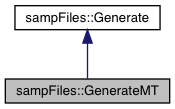
\includegraphics[width=203pt]{classsamp_files_1_1_generate_m_t__inherit__graph}
\end{center}
\end{figure}


Collaboration diagram for samp\+Files\+:\+:Generate\+MT\+:\nopagebreak
\begin{figure}[H]
\begin{center}
\leavevmode
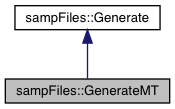
\includegraphics[width=203pt]{classsamp_files_1_1_generate_m_t__coll__graph}
\end{center}
\end{figure}
\subsection*{Public Member Functions}
\begin{DoxyCompactItemize}
\item 
\hyperlink{classsamp_files_1_1_generate_m_t_a733ee504a952b6d7ad997a1cd30caf45}{Generate\+MT} ()
\begin{DoxyCompactList}\small\item\em Default constructor. \end{DoxyCompactList}\item 
\mbox{\Hypertarget{classsamp_files_1_1_generate_m_t_a0b2b937aa08cbbbcd9a3b8b45e26e844}\label{classsamp_files_1_1_generate_m_t_a0b2b937aa08cbbbcd9a3b8b45e26e844}} 
\hyperlink{classsamp_files_1_1_generate_m_t_a0b2b937aa08cbbbcd9a3b8b45e26e844}{$\sim$\+Generate\+MT} ()
\begin{DoxyCompactList}\small\item\em Protected destructor. \end{DoxyCompactList}\item 
\hyperlink{classsamp_files_1_1_generate_m_t_ad832487c190c46d781650416560433e5}{Generate\+MT} (const \hyperlink{classsamp_files_1_1_generate_m_t}{Generate\+MT} \&old)=default
\begin{DoxyCompactList}\small\item\em Copy constructor. \end{DoxyCompactList}\item 
\hyperlink{classsamp_files_1_1_generate_m_t_aae91db45fd9d87b0d54cd3d853a218f1}{Generate\+MT} (\hyperlink{classsamp_files_1_1_generate_m_t}{Generate\+MT} \&\&old)=default
\begin{DoxyCompactList}\small\item\em Move constructor. \end{DoxyCompactList}\item 
\hyperlink{classsamp_files_1_1_generate_m_t}{Generate\+MT} \& \hyperlink{classsamp_files_1_1_generate_m_t_a37331925c0b909adc51188af1b80995a}{operator=} (const \hyperlink{classsamp_files_1_1_generate_m_t}{Generate\+MT} \&old)=default
\begin{DoxyCompactList}\small\item\em Copy assignment operator. \end{DoxyCompactList}\item 
\hyperlink{classsamp_files_1_1_generate_m_t}{Generate\+MT} \& \hyperlink{classsamp_files_1_1_generate_m_t_a7c633b7728fcadde846a4538484d286a}{operator=} (\hyperlink{classsamp_files_1_1_generate_m_t}{Generate\+MT} \&\&old)=default
\begin{DoxyCompactList}\small\item\em Move assignment. \end{DoxyCompactList}\item 
volatile uint64\+\_\+t \hyperlink{classsamp_files_1_1_generate_m_t_a500e163265b6fdae0a30fdacc1c37f80}{ran\+Int} ()
\begin{DoxyCompactList}\small\item\em \hyperlink{classsamp_files_1_1_generate}{Generate} a pseudo-\/random 64-\/bit unsigned integer. \end{DoxyCompactList}\end{DoxyCompactItemize}
\subsection*{Protected Attributes}
\begin{DoxyCompactItemize}
\item 
\mbox{\Hypertarget{classsamp_files_1_1_generate_m_t_a41317c198d417a6d4a1d538e62e3bd1d}\label{classsamp_files_1_1_generate_m_t_a41317c198d417a6d4a1d538e62e3bd1d}} 
uint64\+\_\+t \hyperlink{classsamp_files_1_1_generate_m_t_a41317c198d417a6d4a1d538e62e3bd1d}{\+\_\+mt} \mbox{[}312\mbox{]}
\begin{DoxyCompactList}\small\item\em Generator state array. \end{DoxyCompactList}\item 
\mbox{\Hypertarget{classsamp_files_1_1_generate_m_t_a3ce134726a89493d13a78f8aea0ce0ee}\label{classsamp_files_1_1_generate_m_t_a3ce134726a89493d13a78f8aea0ce0ee}} 
size\+\_\+t \hyperlink{classsamp_files_1_1_generate_m_t_a3ce134726a89493d13a78f8aea0ce0ee}{\+\_\+mti}
\begin{DoxyCompactList}\small\item\em State of the array index. \end{DoxyCompactList}\item 
\mbox{\Hypertarget{classsamp_files_1_1_generate_m_t_aca8e0fbe5fa5c0312a977dea46ccddec}\label{classsamp_files_1_1_generate_m_t_aca8e0fbe5fa5c0312a977dea46ccddec}} 
uint64\+\_\+t \hyperlink{classsamp_files_1_1_generate_m_t_aca8e0fbe5fa5c0312a977dea46ccddec}{\+\_\+x}
\begin{DoxyCompactList}\small\item\em Current state. \end{DoxyCompactList}\end{DoxyCompactItemize}
\subsection*{Static Protected Attributes}
\begin{DoxyCompactItemize}
\item 
\mbox{\Hypertarget{classsamp_files_1_1_generate_m_t_a1baccbd00a9ba762e624a13bfa79a6c7}\label{classsamp_files_1_1_generate_m_t_a1baccbd00a9ba762e624a13bfa79a6c7}} 
static const unsigned short \hyperlink{classsamp_files_1_1_generate_m_t_a1baccbd00a9ba762e624a13bfa79a6c7}{\+\_\+n} = 312
\begin{DoxyCompactList}\small\item\em Degree of recurrence. \end{DoxyCompactList}\item 
\mbox{\Hypertarget{classsamp_files_1_1_generate_m_t_aa0f8cc15e9726d931e5042e16be55cf9}\label{classsamp_files_1_1_generate_m_t_aa0f8cc15e9726d931e5042e16be55cf9}} 
static const unsigned short \hyperlink{classsamp_files_1_1_generate_m_t_aa0f8cc15e9726d931e5042e16be55cf9}{\+\_\+m} = 156
\begin{DoxyCompactList}\small\item\em Middle word. \end{DoxyCompactList}\item 
\mbox{\Hypertarget{classsamp_files_1_1_generate_m_t_add38df40f5c48eedb86eb1bf8f4fb67e}\label{classsamp_files_1_1_generate_m_t_add38df40f5c48eedb86eb1bf8f4fb67e}} 
static const uint64\+\_\+t \hyperlink{classsamp_files_1_1_generate_m_t_add38df40f5c48eedb86eb1bf8f4fb67e}{\+\_\+um} = static\+\_\+cast$<$uint64\+\_\+t$>$(0x7\+F\+F\+F\+F\+F\+F\+F)
\begin{DoxyCompactList}\small\item\em Most significant 33 bits. \end{DoxyCompactList}\item 
\mbox{\Hypertarget{classsamp_files_1_1_generate_m_t_a69615e65ec1e10bbac2da0c4ec4f8b20}\label{classsamp_files_1_1_generate_m_t_a69615e65ec1e10bbac2da0c4ec4f8b20}} 
static const uint64\+\_\+t \hyperlink{classsamp_files_1_1_generate_m_t_a69615e65ec1e10bbac2da0c4ec4f8b20}{\+\_\+lm} = static\+\_\+cast$<$uint64\+\_\+t$>$(0x\+F\+F\+F\+F\+F\+F\+F\+F80000000)
\begin{DoxyCompactList}\small\item\em Least significant 31 bits. \end{DoxyCompactList}\item 
\mbox{\Hypertarget{classsamp_files_1_1_generate_m_t_a5a90cd28215ac0b3272c1a3480bf56ce}\label{classsamp_files_1_1_generate_m_t_a5a90cd28215ac0b3272c1a3480bf56ce}} 
static const uint64\+\_\+t \hyperlink{classsamp_files_1_1_generate_m_t_a5a90cd28215ac0b3272c1a3480bf56ce}{\+\_\+b} = static\+\_\+cast$<$uint64\+\_\+t$>$(0x71\+D67\+F\+F\+F\+E\+D\+A60000)
\begin{DoxyCompactList}\small\item\em Tempering bitmask. \end{DoxyCompactList}\item 
\mbox{\Hypertarget{classsamp_files_1_1_generate_m_t_a8abca1c01d475316b80e0d7b7e23e88d}\label{classsamp_files_1_1_generate_m_t_a8abca1c01d475316b80e0d7b7e23e88d}} 
static const uint64\+\_\+t \hyperlink{classsamp_files_1_1_generate_m_t_a8abca1c01d475316b80e0d7b7e23e88d}{\+\_\+c} = static\+\_\+cast$<$uint64\+\_\+t$>$(0x\+F\+F\+F7\+E\+E\+E000000000)
\begin{DoxyCompactList}\small\item\em Tempering bitmask. \end{DoxyCompactList}\item 
\mbox{\Hypertarget{classsamp_files_1_1_generate_m_t_ab4c0a3714189a167cb6d0d0cf33df694}\label{classsamp_files_1_1_generate_m_t_ab4c0a3714189a167cb6d0d0cf33df694}} 
static const uint64\+\_\+t \hyperlink{classsamp_files_1_1_generate_m_t_ab4c0a3714189a167cb6d0d0cf33df694}{\+\_\+d} = static\+\_\+cast$<$uint64\+\_\+t$>$(0x5555555555555555)
\begin{DoxyCompactList}\small\item\em Tempering bitmask. \end{DoxyCompactList}\item 
\mbox{\Hypertarget{classsamp_files_1_1_generate_m_t_a5ab9c0985b9fd3de64316f580c2eba7d}\label{classsamp_files_1_1_generate_m_t_a5ab9c0985b9fd3de64316f580c2eba7d}} 
static const unsigned int \hyperlink{classsamp_files_1_1_generate_m_t_a5ab9c0985b9fd3de64316f580c2eba7d}{\+\_\+l} = 43
\begin{DoxyCompactList}\small\item\em Tempering shift. \end{DoxyCompactList}\item 
\mbox{\Hypertarget{classsamp_files_1_1_generate_m_t_aaae970a607ffdb407b1bdf1e5762c92d}\label{classsamp_files_1_1_generate_m_t_aaae970a607ffdb407b1bdf1e5762c92d}} 
static const unsigned int \hyperlink{classsamp_files_1_1_generate_m_t_aaae970a607ffdb407b1bdf1e5762c92d}{\+\_\+s} = 17
\begin{DoxyCompactList}\small\item\em Tempering shift. \end{DoxyCompactList}\item 
\mbox{\Hypertarget{classsamp_files_1_1_generate_m_t_a1ee601d010446762cfc1ad6c98d6673f}\label{classsamp_files_1_1_generate_m_t_a1ee601d010446762cfc1ad6c98d6673f}} 
static const unsigned int \hyperlink{classsamp_files_1_1_generate_m_t_a1ee601d010446762cfc1ad6c98d6673f}{\+\_\+t} = 37
\begin{DoxyCompactList}\small\item\em Tempering shift. \end{DoxyCompactList}\item 
\mbox{\Hypertarget{classsamp_files_1_1_generate_m_t_a115d257a43adaf460b41c8725f016abd}\label{classsamp_files_1_1_generate_m_t_a115d257a43adaf460b41c8725f016abd}} 
static const unsigned int \hyperlink{classsamp_files_1_1_generate_m_t_a115d257a43adaf460b41c8725f016abd}{\+\_\+u} = 29
\begin{DoxyCompactList}\small\item\em Tempering shift. \end{DoxyCompactList}\item 
\mbox{\Hypertarget{classsamp_files_1_1_generate_m_t_adf7067ae1e83dd2129650643b5930684}\label{classsamp_files_1_1_generate_m_t_adf7067ae1e83dd2129650643b5930684}} 
static const uint64\+\_\+t \hyperlink{classsamp_files_1_1_generate_m_t_adf7067ae1e83dd2129650643b5930684}{\+\_\+alt} \mbox{[}2\mbox{]} = \{static\+\_\+cast$<$uint64\+\_\+t$>$(0), static\+\_\+cast$<$uint64\+\_\+t$>$(0x\+B5026\+F5\+A\+A96619\+E9)\}
\begin{DoxyCompactList}\small\item\em Array of alternative values for the twist. \end{DoxyCompactList}\end{DoxyCompactItemize}
\subsection*{Additional Inherited Members}


\subsection{Detailed Description}
Pseudo-\/random number generator. 

An implementaiton of the 64-\/bit M\+T19937 (\char`\"{}\+Mersenne Twister\char`\"{}) \cite{matsumoto98a} pseudo-\/random number generator (P\+R\+NG). The constructor automatically seeds the P\+R\+NG. The implementation was guided by the reference code \href{http://www.math.sci.hiroshima-u.ac.jp/~m-mat/MT/emt64.html}{\tt posted by the authors}. 

\subsection{Constructor \& Destructor Documentation}
\mbox{\Hypertarget{classsamp_files_1_1_generate_m_t_a733ee504a952b6d7ad997a1cd30caf45}\label{classsamp_files_1_1_generate_m_t_a733ee504a952b6d7ad997a1cd30caf45}} 
\index{samp\+Files\+::\+Generate\+MT@{samp\+Files\+::\+Generate\+MT}!Generate\+MT@{Generate\+MT}}
\index{Generate\+MT@{Generate\+MT}!samp\+Files\+::\+Generate\+MT@{samp\+Files\+::\+Generate\+MT}}
\subsubsection{\texorpdfstring{Generate\+M\+T()}{GenerateMT()}\hspace{0.1cm}{\footnotesize\ttfamily [1/3]}}
{\footnotesize\ttfamily Generate\+M\+T\+::\+Generate\+MT (\begin{DoxyParamCaption}{ }\end{DoxyParamCaption})}



Default constructor. 

Seeds the P\+R\+NG with a call to the {\itshape R\+D\+T\+SC} instruction. \mbox{\Hypertarget{classsamp_files_1_1_generate_m_t_ad832487c190c46d781650416560433e5}\label{classsamp_files_1_1_generate_m_t_ad832487c190c46d781650416560433e5}} 
\index{samp\+Files\+::\+Generate\+MT@{samp\+Files\+::\+Generate\+MT}!Generate\+MT@{Generate\+MT}}
\index{Generate\+MT@{Generate\+MT}!samp\+Files\+::\+Generate\+MT@{samp\+Files\+::\+Generate\+MT}}
\subsubsection{\texorpdfstring{Generate\+M\+T()}{GenerateMT()}\hspace{0.1cm}{\footnotesize\ttfamily [2/3]}}
{\footnotesize\ttfamily samp\+Files\+::\+Generate\+M\+T\+::\+Generate\+MT (\begin{DoxyParamCaption}\item[{const \hyperlink{classsamp_files_1_1_generate_m_t}{Generate\+MT} \&}]{old }\end{DoxyParamCaption})\hspace{0.3cm}{\ttfamily [default]}}



Copy constructor. 


\begin{DoxyParams}[1]{Parameters}
\mbox{\tt in}  & {\em old} & object to copy \\
\hline
\end{DoxyParams}
\mbox{\Hypertarget{classsamp_files_1_1_generate_m_t_aae91db45fd9d87b0d54cd3d853a218f1}\label{classsamp_files_1_1_generate_m_t_aae91db45fd9d87b0d54cd3d853a218f1}} 
\index{samp\+Files\+::\+Generate\+MT@{samp\+Files\+::\+Generate\+MT}!Generate\+MT@{Generate\+MT}}
\index{Generate\+MT@{Generate\+MT}!samp\+Files\+::\+Generate\+MT@{samp\+Files\+::\+Generate\+MT}}
\subsubsection{\texorpdfstring{Generate\+M\+T()}{GenerateMT()}\hspace{0.1cm}{\footnotesize\ttfamily [3/3]}}
{\footnotesize\ttfamily samp\+Files\+::\+Generate\+M\+T\+::\+Generate\+MT (\begin{DoxyParamCaption}\item[{\hyperlink{classsamp_files_1_1_generate_m_t}{Generate\+MT} \&\&}]{old }\end{DoxyParamCaption})\hspace{0.3cm}{\ttfamily [default]}}



Move constructor. 


\begin{DoxyParams}[1]{Parameters}
\mbox{\tt in}  & {\em old} & object to move \\
\hline
\end{DoxyParams}


\subsection{Member Function Documentation}
\mbox{\Hypertarget{classsamp_files_1_1_generate_m_t_a37331925c0b909adc51188af1b80995a}\label{classsamp_files_1_1_generate_m_t_a37331925c0b909adc51188af1b80995a}} 
\index{samp\+Files\+::\+Generate\+MT@{samp\+Files\+::\+Generate\+MT}!operator=@{operator=}}
\index{operator=@{operator=}!samp\+Files\+::\+Generate\+MT@{samp\+Files\+::\+Generate\+MT}}
\subsubsection{\texorpdfstring{operator=()}{operator=()}\hspace{0.1cm}{\footnotesize\ttfamily [1/2]}}
{\footnotesize\ttfamily \hyperlink{classsamp_files_1_1_generate_m_t}{Generate\+MT}\& samp\+Files\+::\+Generate\+M\+T\+::operator= (\begin{DoxyParamCaption}\item[{const \hyperlink{classsamp_files_1_1_generate_m_t}{Generate\+MT} \&}]{old }\end{DoxyParamCaption})\hspace{0.3cm}{\ttfamily [default]}}



Copy assignment operator. 


\begin{DoxyParams}[1]{Parameters}
\mbox{\tt in}  & {\em old} & object to copy \\
\hline
\end{DoxyParams}
\mbox{\Hypertarget{classsamp_files_1_1_generate_m_t_a7c633b7728fcadde846a4538484d286a}\label{classsamp_files_1_1_generate_m_t_a7c633b7728fcadde846a4538484d286a}} 
\index{samp\+Files\+::\+Generate\+MT@{samp\+Files\+::\+Generate\+MT}!operator=@{operator=}}
\index{operator=@{operator=}!samp\+Files\+::\+Generate\+MT@{samp\+Files\+::\+Generate\+MT}}
\subsubsection{\texorpdfstring{operator=()}{operator=()}\hspace{0.1cm}{\footnotesize\ttfamily [2/2]}}
{\footnotesize\ttfamily \hyperlink{classsamp_files_1_1_generate_m_t}{Generate\+MT}\& samp\+Files\+::\+Generate\+M\+T\+::operator= (\begin{DoxyParamCaption}\item[{\hyperlink{classsamp_files_1_1_generate_m_t}{Generate\+MT} \&\&}]{old }\end{DoxyParamCaption})\hspace{0.3cm}{\ttfamily [default]}}



Move assignment. 


\begin{DoxyParams}[1]{Parameters}
\mbox{\tt in}  & {\em old} & object to move \\
\hline
\end{DoxyParams}
\mbox{\Hypertarget{classsamp_files_1_1_generate_m_t_a500e163265b6fdae0a30fdacc1c37f80}\label{classsamp_files_1_1_generate_m_t_a500e163265b6fdae0a30fdacc1c37f80}} 
\index{samp\+Files\+::\+Generate\+MT@{samp\+Files\+::\+Generate\+MT}!ran\+Int@{ran\+Int}}
\index{ran\+Int@{ran\+Int}!samp\+Files\+::\+Generate\+MT@{samp\+Files\+::\+Generate\+MT}}
\subsubsection{\texorpdfstring{ran\+Int()}{ranInt()}}
{\footnotesize\ttfamily volatile uint64\+\_\+t Generate\+M\+T\+::ran\+Int (\begin{DoxyParamCaption}{ }\end{DoxyParamCaption})\hspace{0.3cm}{\ttfamily [virtual]}}



\hyperlink{classsamp_files_1_1_generate}{Generate} a pseudo-\/random 64-\/bit unsigned integer. 

\begin{DoxyReturn}{Returns}
pseudo-\/random 64-\/bit unsigned integer 
\end{DoxyReturn}


Implements \hyperlink{classsamp_files_1_1_generate_a86fe4e68cc0809d4d936615fc60c125e}{samp\+Files\+::\+Generate}.



The documentation for this class was generated from the following files\+:\begin{DoxyCompactItemize}
\item 
\hyperlink{random_8hpp}{random.\+hpp}\item 
\hyperlink{random_8cpp}{random.\+cpp}\end{DoxyCompactItemize}

\hypertarget{classsamp_files_1_1_gtxt_file}{}\section{samp\+Files\+:\+:Gtxt\+File Class Reference}
\label{classsamp_files_1_1_gtxt_file}\index{samp\+Files\+::\+Gtxt\+File@{samp\+Files\+::\+Gtxt\+File}}


Generic text file base class.  




{\ttfamily \#include $<$varfiles.\+hpp$>$}



Inheritance diagram for samp\+Files\+:\+:Gtxt\+File\+:\nopagebreak
\begin{figure}[H]
\begin{center}
\leavevmode
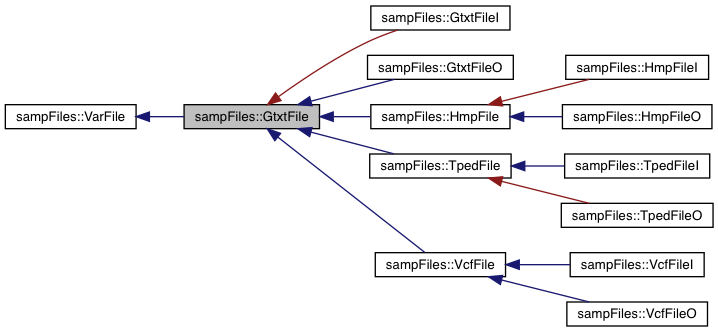
\includegraphics[width=350pt]{classsamp_files_1_1_gtxt_file__inherit__graph}
\end{center}
\end{figure}


Collaboration diagram for samp\+Files\+:\+:Gtxt\+File\+:\nopagebreak
\begin{figure}[H]
\begin{center}
\leavevmode
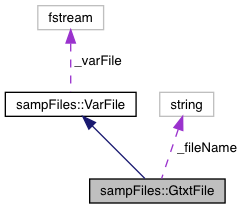
\includegraphics[width=254pt]{classsamp_files_1_1_gtxt_file__coll__graph}
\end{center}
\end{figure}
\subsection*{Public Member Functions}
\begin{DoxyCompactItemize}
\item 
\mbox{\Hypertarget{classsamp_files_1_1_gtxt_file_a43c69cb8dd8736b9e39014b2308661d6}\label{classsamp_files_1_1_gtxt_file_a43c69cb8dd8736b9e39014b2308661d6}} 
\hyperlink{classsamp_files_1_1_gtxt_file_a43c69cb8dd8736b9e39014b2308661d6}{Gtxt\+File} ()
\begin{DoxyCompactList}\small\item\em Default constructor. \end{DoxyCompactList}\item 
\hyperlink{classsamp_files_1_1_gtxt_file_a8fa6b2a9127d2c66de0c4d6b14555e66}{Gtxt\+File} (const string \&file\+Name)
\begin{DoxyCompactList}\small\item\em Constructor with file name. \end{DoxyCompactList}\item 
\hyperlink{classsamp_files_1_1_gtxt_file_a401ff9bae54850c2bcd54722f80aa479}{Gtxt\+File} (const string \&file\+Name, const bool \&head)
\begin{DoxyCompactList}\small\item\em Constructor with file name and header indicator. \end{DoxyCompactList}\item 
\mbox{\Hypertarget{classsamp_files_1_1_gtxt_file_a4f0a23f83e9f5085e086f1f8f0f39d12}\label{classsamp_files_1_1_gtxt_file_a4f0a23f83e9f5085e086f1f8f0f39d12}} 
\hyperlink{classsamp_files_1_1_gtxt_file_a4f0a23f83e9f5085e086f1f8f0f39d12}{Gtxt\+File} (const \hyperlink{classsamp_files_1_1_gtxt_file}{Gtxt\+File} \&in)=default
\begin{DoxyCompactList}\small\item\em Copy constructor. \end{DoxyCompactList}\item 
\mbox{\Hypertarget{classsamp_files_1_1_gtxt_file_a062fb2cc37eedf763eba9184ff29dc5e}\label{classsamp_files_1_1_gtxt_file_a062fb2cc37eedf763eba9184ff29dc5e}} 
\hyperlink{classsamp_files_1_1_gtxt_file}{Gtxt\+File} \& \hyperlink{classsamp_files_1_1_gtxt_file_a062fb2cc37eedf763eba9184ff29dc5e}{operator=} (const \hyperlink{classsamp_files_1_1_gtxt_file}{Gtxt\+File} \&in)=default
\begin{DoxyCompactList}\small\item\em Copy assignment. \end{DoxyCompactList}\item 
\mbox{\Hypertarget{classsamp_files_1_1_gtxt_file_a1514f20af2494f9ca9f232f7b3ae6cec}\label{classsamp_files_1_1_gtxt_file_a1514f20af2494f9ca9f232f7b3ae6cec}} 
\hyperlink{classsamp_files_1_1_gtxt_file_a1514f20af2494f9ca9f232f7b3ae6cec}{Gtxt\+File} (\hyperlink{classsamp_files_1_1_gtxt_file}{Gtxt\+File} \&\&in)=default
\begin{DoxyCompactList}\small\item\em Move constructor. \end{DoxyCompactList}\item 
\mbox{\Hypertarget{classsamp_files_1_1_gtxt_file_a29107fef9662b347b440a8284c3c967e}\label{classsamp_files_1_1_gtxt_file_a29107fef9662b347b440a8284c3c967e}} 
\hyperlink{classsamp_files_1_1_gtxt_file}{Gtxt\+File} \& \hyperlink{classsamp_files_1_1_gtxt_file_a29107fef9662b347b440a8284c3c967e}{operator=} (\hyperlink{classsamp_files_1_1_gtxt_file}{Gtxt\+File} \&\&in)=default
\begin{DoxyCompactList}\small\item\em Move assignment. \end{DoxyCompactList}\item 
\mbox{\Hypertarget{classsamp_files_1_1_gtxt_file_aee4e94c994fc6776aa95444fcec4f6a3}\label{classsamp_files_1_1_gtxt_file_aee4e94c994fc6776aa95444fcec4f6a3}} 
\hyperlink{classsamp_files_1_1_gtxt_file_aee4e94c994fc6776aa95444fcec4f6a3}{$\sim$\+Gtxt\+File} ()
\begin{DoxyCompactList}\small\item\em Destructor. \end{DoxyCompactList}\item 
\mbox{\Hypertarget{classsamp_files_1_1_gtxt_file_ad93a05c665b81cca13c96910a7715755}\label{classsamp_files_1_1_gtxt_file_ad93a05c665b81cca13c96910a7715755}} 
virtual void \hyperlink{classsamp_files_1_1_gtxt_file_ad93a05c665b81cca13c96910a7715755}{open} ()
\begin{DoxyCompactList}\small\item\em Open stream (does nothing) \end{DoxyCompactList}\item 
\mbox{\Hypertarget{classsamp_files_1_1_gtxt_file_ab70cf8235e1e7f519f2d114ec99973a7}\label{classsamp_files_1_1_gtxt_file_ab70cf8235e1e7f519f2d114ec99973a7}} 
virtual void \hyperlink{classsamp_files_1_1_gtxt_file_ab70cf8235e1e7f519f2d114ec99973a7}{close} ()
\begin{DoxyCompactList}\small\item\em Close stream. \end{DoxyCompactList}\end{DoxyCompactItemize}
\subsection*{Protected Attributes}
\begin{DoxyCompactItemize}
\item 
\mbox{\Hypertarget{classsamp_files_1_1_gtxt_file_a6bb0295beed42ba848f8e2fb73d17e2a}\label{classsamp_files_1_1_gtxt_file_a6bb0295beed42ba848f8e2fb73d17e2a}} 
string \hyperlink{classsamp_files_1_1_gtxt_file_a6bb0295beed42ba848f8e2fb73d17e2a}{\+\_\+file\+Name}
\begin{DoxyCompactList}\small\item\em File name. \end{DoxyCompactList}\item 
\mbox{\Hypertarget{classsamp_files_1_1_gtxt_file_a44b688239f4ede24fc31a34583ced570}\label{classsamp_files_1_1_gtxt_file_a44b688239f4ede24fc31a34583ced570}} 
bool \hyperlink{classsamp_files_1_1_gtxt_file_a44b688239f4ede24fc31a34583ced570}{\+\_\+head}
\begin{DoxyCompactList}\small\item\em Is there a header? \end{DoxyCompactList}\end{DoxyCompactItemize}
\subsection*{Additional Inherited Members}


\subsection{Detailed Description}
Generic text file base class. 

Sets up streams for text files. If specified, the first line can be considered a header and treated separately. 

\subsection{Constructor \& Destructor Documentation}
\mbox{\Hypertarget{classsamp_files_1_1_gtxt_file_a8fa6b2a9127d2c66de0c4d6b14555e66}\label{classsamp_files_1_1_gtxt_file_a8fa6b2a9127d2c66de0c4d6b14555e66}} 
\index{samp\+Files\+::\+Gtxt\+File@{samp\+Files\+::\+Gtxt\+File}!Gtxt\+File@{Gtxt\+File}}
\index{Gtxt\+File@{Gtxt\+File}!samp\+Files\+::\+Gtxt\+File@{samp\+Files\+::\+Gtxt\+File}}
\subsubsection{\texorpdfstring{Gtxt\+File()}{GtxtFile()}\hspace{0.1cm}{\footnotesize\ttfamily [1/2]}}
{\footnotesize\ttfamily samp\+Files\+::\+Gtxt\+File\+::\+Gtxt\+File (\begin{DoxyParamCaption}\item[{const string \&}]{file\+Name }\end{DoxyParamCaption})\hspace{0.3cm}{\ttfamily [inline]}}



Constructor with file name. 


\begin{DoxyParams}[1]{Parameters}
\mbox{\tt in}  & {\em file\+Name} & file name \\
\hline
\end{DoxyParams}
\mbox{\Hypertarget{classsamp_files_1_1_gtxt_file_a401ff9bae54850c2bcd54722f80aa479}\label{classsamp_files_1_1_gtxt_file_a401ff9bae54850c2bcd54722f80aa479}} 
\index{samp\+Files\+::\+Gtxt\+File@{samp\+Files\+::\+Gtxt\+File}!Gtxt\+File@{Gtxt\+File}}
\index{Gtxt\+File@{Gtxt\+File}!samp\+Files\+::\+Gtxt\+File@{samp\+Files\+::\+Gtxt\+File}}
\subsubsection{\texorpdfstring{Gtxt\+File()}{GtxtFile()}\hspace{0.1cm}{\footnotesize\ttfamily [2/2]}}
{\footnotesize\ttfamily samp\+Files\+::\+Gtxt\+File\+::\+Gtxt\+File (\begin{DoxyParamCaption}\item[{const string \&}]{file\+Name,  }\item[{const bool \&}]{head }\end{DoxyParamCaption})\hspace{0.3cm}{\ttfamily [inline]}}



Constructor with file name and header indicator. 


\begin{DoxyParams}[1]{Parameters}
\mbox{\tt in}  & {\em file\+Name} & file name \\
\hline
\mbox{\tt in}  & {\em head} & header presence \\
\hline
\end{DoxyParams}
Here is the call graph for this function\+:\nopagebreak
\begin{figure}[H]
\begin{center}
\leavevmode
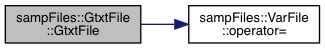
\includegraphics[width=316pt]{classsamp_files_1_1_gtxt_file_a401ff9bae54850c2bcd54722f80aa479_cgraph}
\end{center}
\end{figure}


The documentation for this class was generated from the following files\+:\begin{DoxyCompactItemize}
\item 
\hyperlink{varfiles_8hpp}{varfiles.\+hpp}\item 
\hyperlink{varfiles_8cpp}{varfiles.\+cpp}\end{DoxyCompactItemize}

\hypertarget{classsamp_files_1_1_gtxt_file_i}{}\section{samp\+Files\+:\+:Gtxt\+FileI Class Reference}
\label{classsamp_files_1_1_gtxt_file_i}\index{samp\+Files\+::\+Gtxt\+FileI@{samp\+Files\+::\+Gtxt\+FileI}}


Text file input class.  




{\ttfamily \#include $<$varfiles.\+hpp$>$}



Inheritance diagram for samp\+Files\+:\+:Gtxt\+FileI\+:\nopagebreak
\begin{figure}[H]
\begin{center}
\leavevmode
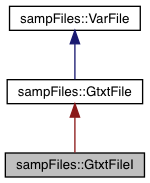
\includegraphics[width=184pt]{classsamp_files_1_1_gtxt_file_i__inherit__graph}
\end{center}
\end{figure}


Collaboration diagram for samp\+Files\+:\+:Gtxt\+FileI\+:\nopagebreak
\begin{figure}[H]
\begin{center}
\leavevmode
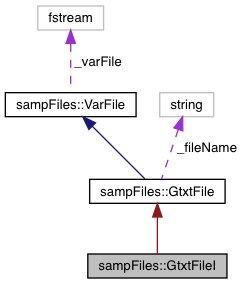
\includegraphics[width=254pt]{classsamp_files_1_1_gtxt_file_i__coll__graph}
\end{center}
\end{figure}
\subsection*{Public Member Functions}
\begin{DoxyCompactItemize}
\item 
\mbox{\Hypertarget{classsamp_files_1_1_gtxt_file_i_a4b125fb20371c9e97945ef7003165ee6}\label{classsamp_files_1_1_gtxt_file_i_a4b125fb20371c9e97945ef7003165ee6}} 
\hyperlink{classsamp_files_1_1_gtxt_file_i_a4b125fb20371c9e97945ef7003165ee6}{Gtxt\+FileI} ()
\begin{DoxyCompactList}\small\item\em Default constructor. \end{DoxyCompactList}\item 
\hyperlink{classsamp_files_1_1_gtxt_file_i_aa41eb934d041edd06cee29d3e69f73da}{Gtxt\+FileI} (const string \&file\+Name)
\begin{DoxyCompactList}\small\item\em File name constructor with header specification. \end{DoxyCompactList}\item 
\hyperlink{classsamp_files_1_1_gtxt_file_i_a78dbd140e9f2e49d98c15c6360b0e88f}{Gtxt\+FileI} (const string \&file\+Name, const bool \&head)
\begin{DoxyCompactList}\small\item\em File name constructor with header specification. \end{DoxyCompactList}\item 
\mbox{\Hypertarget{classsamp_files_1_1_gtxt_file_i_a55927f7c5eb0b1b10331d4e09cf265d7}\label{classsamp_files_1_1_gtxt_file_i_a55927f7c5eb0b1b10331d4e09cf265d7}} 
\hyperlink{classsamp_files_1_1_gtxt_file_i_a55927f7c5eb0b1b10331d4e09cf265d7}{Gtxt\+FileI} (const \hyperlink{classsamp_files_1_1_gtxt_file_i}{Gtxt\+FileI} \&in)=default
\begin{DoxyCompactList}\small\item\em Copy constructor. \end{DoxyCompactList}\item 
\mbox{\Hypertarget{classsamp_files_1_1_gtxt_file_i_a6a0acfa7671ef2ab4a3405e23c9c33ec}\label{classsamp_files_1_1_gtxt_file_i_a6a0acfa7671ef2ab4a3405e23c9c33ec}} 
\hyperlink{classsamp_files_1_1_gtxt_file_i}{Gtxt\+FileI} \& \hyperlink{classsamp_files_1_1_gtxt_file_i_a6a0acfa7671ef2ab4a3405e23c9c33ec}{operator=} (const \hyperlink{classsamp_files_1_1_gtxt_file_i}{Gtxt\+FileI} \&in)=default
\begin{DoxyCompactList}\small\item\em Copy assignment. \end{DoxyCompactList}\item 
\mbox{\Hypertarget{classsamp_files_1_1_gtxt_file_i_a93ff32becc286112d7e1a2fc3284405c}\label{classsamp_files_1_1_gtxt_file_i_a93ff32becc286112d7e1a2fc3284405c}} 
\hyperlink{classsamp_files_1_1_gtxt_file_i_a93ff32becc286112d7e1a2fc3284405c}{Gtxt\+FileI} (\hyperlink{classsamp_files_1_1_gtxt_file_i}{Gtxt\+FileI} \&\&in)=default
\begin{DoxyCompactList}\small\item\em Move constructor. \end{DoxyCompactList}\item 
\mbox{\Hypertarget{classsamp_files_1_1_gtxt_file_i_a76524baf921d6550de5a8bb7748ac871}\label{classsamp_files_1_1_gtxt_file_i_a76524baf921d6550de5a8bb7748ac871}} 
\hyperlink{classsamp_files_1_1_gtxt_file_i}{Gtxt\+FileI} \& \hyperlink{classsamp_files_1_1_gtxt_file_i_a76524baf921d6550de5a8bb7748ac871}{operator=} (\hyperlink{classsamp_files_1_1_gtxt_file_i}{Gtxt\+FileI} \&\&in)=default
\begin{DoxyCompactList}\small\item\em Move assignment. \end{DoxyCompactList}\item 
\mbox{\Hypertarget{classsamp_files_1_1_gtxt_file_i_ad291e4fefc01d04671a9af5429649431}\label{classsamp_files_1_1_gtxt_file_i_ad291e4fefc01d04671a9af5429649431}} 
\hyperlink{classsamp_files_1_1_gtxt_file_i_ad291e4fefc01d04671a9af5429649431}{$\sim$\+Gtxt\+FileI} ()
\begin{DoxyCompactList}\small\item\em Destructor. \end{DoxyCompactList}\item 
\mbox{\Hypertarget{classsamp_files_1_1_gtxt_file_i_a02dbd0de90315f1e59c0a5c88c13c055}\label{classsamp_files_1_1_gtxt_file_i_a02dbd0de90315f1e59c0a5c88c13c055}} 
void \hyperlink{classsamp_files_1_1_gtxt_file_i_a02dbd0de90315f1e59c0a5c88c13c055}{open} ()
\begin{DoxyCompactList}\small\item\em Open stream to read. \end{DoxyCompactList}\item 
void \hyperlink{classsamp_files_1_1_gtxt_file_i_ae3a13c1ff7dce452859abf0942da0631}{sample} (\hyperlink{classsamp_files_1_1_gtxt_file_o}{Gtxt\+FileO} \&out, const uint64\+\_\+t \&n, const bool \&head\+Skip)
\begin{DoxyCompactList}\small\item\em Sample rows and save to a text file. \end{DoxyCompactList}\item 
void \hyperlink{classsamp_files_1_1_gtxt_file_i_afcdc7d04dfb617103080bc1db2822c84}{sample} (const uint64\+\_\+t \&n, const bool \&head\+Skip, const char \&delim, vector$<$ string $>$ \&out)
\begin{DoxyCompactList}\small\item\em Sample rows and save export to a vector of strings. \end{DoxyCompactList}\item 
\mbox{\Hypertarget{classsamp_files_1_1_gtxt_file_i_a3da7d42ee1e48e302d776486d07204f3}\label{classsamp_files_1_1_gtxt_file_i_a3da7d42ee1e48e302d776486d07204f3}} 
uint64\+\_\+t \hyperlink{classsamp_files_1_1_gtxt_file_i_a3da7d42ee1e48e302d776486d07204f3}{nlines} ()
\begin{DoxyCompactList}\small\item\em Number of S\+N\+Ps in the object. \end{DoxyCompactList}\end{DoxyCompactItemize}
\subsection*{Protected Member Functions}
\begin{DoxyCompactItemize}
\item 
virtual uint64\+\_\+t \hyperlink{classsamp_files_1_1_gtxt_file_i_a5452b2663b374cdaa6b6bd5f34683a3c}{\+\_\+num\+Lines} ()
\begin{DoxyCompactList}\small\item\em Get number of rows in the text file. \end{DoxyCompactList}\end{DoxyCompactItemize}


\subsection{Detailed Description}
Text file input class. 

Reads text files, skipping or copying the header as necessary. 

\subsection{Constructor \& Destructor Documentation}
\mbox{\Hypertarget{classsamp_files_1_1_gtxt_file_i_aa41eb934d041edd06cee29d3e69f73da}\label{classsamp_files_1_1_gtxt_file_i_aa41eb934d041edd06cee29d3e69f73da}} 
\index{samp\+Files\+::\+Gtxt\+FileI@{samp\+Files\+::\+Gtxt\+FileI}!Gtxt\+FileI@{Gtxt\+FileI}}
\index{Gtxt\+FileI@{Gtxt\+FileI}!samp\+Files\+::\+Gtxt\+FileI@{samp\+Files\+::\+Gtxt\+FileI}}
\subsubsection{\texorpdfstring{Gtxt\+File\+I()}{GtxtFileI()}\hspace{0.1cm}{\footnotesize\ttfamily [1/2]}}
{\footnotesize\ttfamily samp\+Files\+::\+Gtxt\+File\+I\+::\+Gtxt\+FileI (\begin{DoxyParamCaption}\item[{const string \&}]{file\+Name }\end{DoxyParamCaption})\hspace{0.3cm}{\ttfamily [inline]}}



File name constructor with header specification. 


\begin{DoxyParams}[1]{Parameters}
\mbox{\tt in}  & {\em file\+Name} & file name including extension \\
\hline
\end{DoxyParams}
\mbox{\Hypertarget{classsamp_files_1_1_gtxt_file_i_a78dbd140e9f2e49d98c15c6360b0e88f}\label{classsamp_files_1_1_gtxt_file_i_a78dbd140e9f2e49d98c15c6360b0e88f}} 
\index{samp\+Files\+::\+Gtxt\+FileI@{samp\+Files\+::\+Gtxt\+FileI}!Gtxt\+FileI@{Gtxt\+FileI}}
\index{Gtxt\+FileI@{Gtxt\+FileI}!samp\+Files\+::\+Gtxt\+FileI@{samp\+Files\+::\+Gtxt\+FileI}}
\subsubsection{\texorpdfstring{Gtxt\+File\+I()}{GtxtFileI()}\hspace{0.1cm}{\footnotesize\ttfamily [2/2]}}
{\footnotesize\ttfamily samp\+Files\+::\+Gtxt\+File\+I\+::\+Gtxt\+FileI (\begin{DoxyParamCaption}\item[{const string \&}]{file\+Name,  }\item[{const bool \&}]{head }\end{DoxyParamCaption})\hspace{0.3cm}{\ttfamily [inline]}}



File name constructor with header specification. 


\begin{DoxyParams}[1]{Parameters}
\mbox{\tt in}  & {\em file\+Name} & file name including extension \\
\hline
\mbox{\tt in}  & {\em head} & header presence \\
\hline
\end{DoxyParams}
Here is the call graph for this function\+:\nopagebreak
\begin{figure}[H]
\begin{center}
\leavevmode
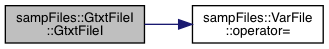
\includegraphics[width=318pt]{classsamp_files_1_1_gtxt_file_i_a78dbd140e9f2e49d98c15c6360b0e88f_cgraph}
\end{center}
\end{figure}


\subsection{Member Function Documentation}
\mbox{\Hypertarget{classsamp_files_1_1_gtxt_file_i_a5452b2663b374cdaa6b6bd5f34683a3c}\label{classsamp_files_1_1_gtxt_file_i_a5452b2663b374cdaa6b6bd5f34683a3c}} 
\index{samp\+Files\+::\+Gtxt\+FileI@{samp\+Files\+::\+Gtxt\+FileI}!\+\_\+num\+Lines@{\+\_\+num\+Lines}}
\index{\+\_\+num\+Lines@{\+\_\+num\+Lines}!samp\+Files\+::\+Gtxt\+FileI@{samp\+Files\+::\+Gtxt\+FileI}}
\subsubsection{\texorpdfstring{\+\_\+num\+Lines()}{\_numLines()}}
{\footnotesize\ttfamily uint64\+\_\+t Gtxt\+File\+I\+::\+\_\+num\+Lines (\begin{DoxyParamCaption}{ }\end{DoxyParamCaption})\hspace{0.3cm}{\ttfamily [protected]}, {\ttfamily [virtual]}}



Get number of rows in the text file. 

Assumes Unix-\/like line endings. Header, if present, is not counted. Is overriden in some, but not all, derived classes.

\begin{DoxyReturn}{Returns}
number of rows 
\end{DoxyReturn}
\mbox{\Hypertarget{classsamp_files_1_1_gtxt_file_i_ae3a13c1ff7dce452859abf0942da0631}\label{classsamp_files_1_1_gtxt_file_i_ae3a13c1ff7dce452859abf0942da0631}} 
\index{samp\+Files\+::\+Gtxt\+FileI@{samp\+Files\+::\+Gtxt\+FileI}!sample@{sample}}
\index{sample@{sample}!samp\+Files\+::\+Gtxt\+FileI@{samp\+Files\+::\+Gtxt\+FileI}}
\subsubsection{\texorpdfstring{sample()}{sample()}\hspace{0.1cm}{\footnotesize\ttfamily [1/2]}}
{\footnotesize\ttfamily void Gtxt\+File\+I\+::sample (\begin{DoxyParamCaption}\item[{\hyperlink{classsamp_files_1_1_gtxt_file_o}{Gtxt\+FileO} \&}]{out,  }\item[{const uint64\+\_\+t \&}]{n,  }\item[{const bool \&}]{head\+Skip }\end{DoxyParamCaption})}



Sample rows and save to a text file. 

Sample $n$ lines without replacement from the file represented by the current object and save to the {\ttfamily out} object. Uses Vitter\textquotesingle{}s \cite{vitter87a} method. Number of samples has to be smaller that the number of rows in the file.


\begin{DoxyParams}[1]{Parameters}
\mbox{\tt in}  & {\em out} & output object \\
\hline
\mbox{\tt in}  & {\em n} & number of rows to sample \\
\hline
\mbox{\tt in}  & {\em head\+Skip} & skip header? Ignored if there is no header \\
\hline
\end{DoxyParams}
\mbox{\Hypertarget{classsamp_files_1_1_gtxt_file_i_afcdc7d04dfb617103080bc1db2822c84}\label{classsamp_files_1_1_gtxt_file_i_afcdc7d04dfb617103080bc1db2822c84}} 
\index{samp\+Files\+::\+Gtxt\+FileI@{samp\+Files\+::\+Gtxt\+FileI}!sample@{sample}}
\index{sample@{sample}!samp\+Files\+::\+Gtxt\+FileI@{samp\+Files\+::\+Gtxt\+FileI}}
\subsubsection{\texorpdfstring{sample()}{sample()}\hspace{0.1cm}{\footnotesize\ttfamily [2/2]}}
{\footnotesize\ttfamily void Gtxt\+File\+I\+::sample (\begin{DoxyParamCaption}\item[{const uint64\+\_\+t \&}]{n,  }\item[{const bool \&}]{head\+Skip,  }\item[{const char \&}]{delim,  }\item[{vector$<$ string $>$ \&}]{out }\end{DoxyParamCaption})}



Sample rows and save export to a vector of strings. 

Sample $n$ rows without replacement from the file represented by the current object and output a vector of strings. Each field separated by the specified delimiter is stored as an element of the vector. Uses Vitter\textquotesingle{}s \cite{vitter87a} method. Number of samples has to be smaller that the number of rows in the file. The output vector is erased if it is not empty.


\begin{DoxyParams}[1]{Parameters}
\mbox{\tt in}  & {\em n} & number of S\+N\+Ps to sample \\
\hline
\mbox{\tt in}  & {\em head\+Skip} & skip header? Ignored if there is no header \\
\hline
\mbox{\tt in}  & {\em delim} & field delimiter \\
\hline
\mbox{\tt out}  & {\em out} & output vector \\
\hline
\end{DoxyParams}
Here is the call graph for this function\+:\nopagebreak
\begin{figure}[H]
\begin{center}
\leavevmode
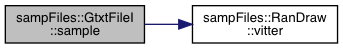
\includegraphics[width=329pt]{classsamp_files_1_1_gtxt_file_i_afcdc7d04dfb617103080bc1db2822c84_cgraph}
\end{center}
\end{figure}


The documentation for this class was generated from the following files\+:\begin{DoxyCompactItemize}
\item 
\hyperlink{varfiles_8hpp}{varfiles.\+hpp}\item 
\hyperlink{varfiles_8cpp}{varfiles.\+cpp}\end{DoxyCompactItemize}

\hypertarget{classsamp_files_1_1_gtxt_file_o}{}\section{samp\+Files\+:\+:Gtxt\+FileO Class Reference}
\label{classsamp_files_1_1_gtxt_file_o}\index{samp\+Files\+::\+Gtxt\+FileO@{samp\+Files\+::\+Gtxt\+FileO}}


Generic text file output class.  




{\ttfamily \#include $<$varfiles.\+hpp$>$}



Inheritance diagram for samp\+Files\+:\+:Gtxt\+FileO\+:\nopagebreak
\begin{figure}[H]
\begin{center}
\leavevmode
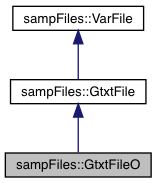
\includegraphics[width=189pt]{classsamp_files_1_1_gtxt_file_o__inherit__graph}
\end{center}
\end{figure}


Collaboration diagram for samp\+Files\+:\+:Gtxt\+FileO\+:\nopagebreak
\begin{figure}[H]
\begin{center}
\leavevmode
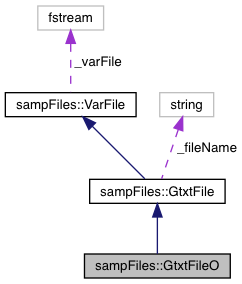
\includegraphics[width=254pt]{classsamp_files_1_1_gtxt_file_o__coll__graph}
\end{center}
\end{figure}
\subsection*{Public Member Functions}
\begin{DoxyCompactItemize}
\item 
\mbox{\Hypertarget{classsamp_files_1_1_gtxt_file_o_a3c79c55c24e4c856763746327091f43b}\label{classsamp_files_1_1_gtxt_file_o_a3c79c55c24e4c856763746327091f43b}} 
\hyperlink{classsamp_files_1_1_gtxt_file_o_a3c79c55c24e4c856763746327091f43b}{Gtxt\+FileO} ()
\begin{DoxyCompactList}\small\item\em Default constructor. \end{DoxyCompactList}\item 
\hyperlink{classsamp_files_1_1_gtxt_file_o_a3329b261b0364edfdc47842609271eb6}{Gtxt\+FileO} (const string \&file\+Name)
\begin{DoxyCompactList}\small\item\em File name constructor. \end{DoxyCompactList}\item 
\hyperlink{classsamp_files_1_1_gtxt_file_o_a84944d8c2b0e6c6eeb877b53e17fc104}{Gtxt\+FileO} (const string \&file\+Name, const bool \&head)
\begin{DoxyCompactList}\small\item\em File name constructor with header specification. \end{DoxyCompactList}\item 
\mbox{\Hypertarget{classsamp_files_1_1_gtxt_file_o_a95cba7e971f6c87c09afc4084433c9c2}\label{classsamp_files_1_1_gtxt_file_o_a95cba7e971f6c87c09afc4084433c9c2}} 
\hyperlink{classsamp_files_1_1_gtxt_file_o_a95cba7e971f6c87c09afc4084433c9c2}{Gtxt\+FileO} (const \hyperlink{classsamp_files_1_1_gtxt_file_o}{Gtxt\+FileO} \&in)=default
\begin{DoxyCompactList}\small\item\em Copy constructor. \end{DoxyCompactList}\item 
\mbox{\Hypertarget{classsamp_files_1_1_gtxt_file_o_a071b19053431ba537a6534a4948adc7c}\label{classsamp_files_1_1_gtxt_file_o_a071b19053431ba537a6534a4948adc7c}} 
\hyperlink{classsamp_files_1_1_gtxt_file_o}{Gtxt\+FileO} \& \hyperlink{classsamp_files_1_1_gtxt_file_o_a071b19053431ba537a6534a4948adc7c}{operator=} (const \hyperlink{classsamp_files_1_1_gtxt_file_o}{Gtxt\+FileO} \&in)=default
\begin{DoxyCompactList}\small\item\em Copy assignment. \end{DoxyCompactList}\item 
\mbox{\Hypertarget{classsamp_files_1_1_gtxt_file_o_a3173192f42a6c9800f329c502e52906b}\label{classsamp_files_1_1_gtxt_file_o_a3173192f42a6c9800f329c502e52906b}} 
\hyperlink{classsamp_files_1_1_gtxt_file_o_a3173192f42a6c9800f329c502e52906b}{Gtxt\+FileO} (\hyperlink{classsamp_files_1_1_gtxt_file_o}{Gtxt\+FileO} \&\&in)=default
\begin{DoxyCompactList}\small\item\em Move constructor. \end{DoxyCompactList}\item 
\mbox{\Hypertarget{classsamp_files_1_1_gtxt_file_o_a610a322b89fc0b7dd807eaed922fdaa4}\label{classsamp_files_1_1_gtxt_file_o_a610a322b89fc0b7dd807eaed922fdaa4}} 
\hyperlink{classsamp_files_1_1_gtxt_file_o}{Gtxt\+FileO} \& \hyperlink{classsamp_files_1_1_gtxt_file_o_a610a322b89fc0b7dd807eaed922fdaa4}{operator=} (\hyperlink{classsamp_files_1_1_gtxt_file_o}{Gtxt\+FileO} \&\&in)=default
\begin{DoxyCompactList}\small\item\em Move assignment. \end{DoxyCompactList}\item 
\mbox{\Hypertarget{classsamp_files_1_1_gtxt_file_o_a3cfd3dc27a9026aeda69ab16ec5d5883}\label{classsamp_files_1_1_gtxt_file_o_a3cfd3dc27a9026aeda69ab16ec5d5883}} 
\hyperlink{classsamp_files_1_1_gtxt_file_o_a3cfd3dc27a9026aeda69ab16ec5d5883}{$\sim$\+Gtxt\+FileO} ()
\begin{DoxyCompactList}\small\item\em Destructor. \end{DoxyCompactList}\item 
\mbox{\Hypertarget{classsamp_files_1_1_gtxt_file_o_a0659134a8ea9f344b5d4e3eb5b7b2452}\label{classsamp_files_1_1_gtxt_file_o_a0659134a8ea9f344b5d4e3eb5b7b2452}} 
void \hyperlink{classsamp_files_1_1_gtxt_file_o_a0659134a8ea9f344b5d4e3eb5b7b2452}{open} ()
\begin{DoxyCompactList}\small\item\em Open stream to write. \end{DoxyCompactList}\end{DoxyCompactItemize}
\subsection*{Friends}
\begin{DoxyCompactItemize}
\item 
\mbox{\Hypertarget{classsamp_files_1_1_gtxt_file_o_a7932dd6919f418cd1d8e5b398bbc72bf}\label{classsamp_files_1_1_gtxt_file_o_a7932dd6919f418cd1d8e5b398bbc72bf}} 
class {\bfseries Gtxt\+FileI}
\end{DoxyCompactItemize}
\subsection*{Additional Inherited Members}


\subsection{Detailed Description}
Generic text file output class. 

Writes text files. 

\subsection{Constructor \& Destructor Documentation}
\mbox{\Hypertarget{classsamp_files_1_1_gtxt_file_o_a3329b261b0364edfdc47842609271eb6}\label{classsamp_files_1_1_gtxt_file_o_a3329b261b0364edfdc47842609271eb6}} 
\index{samp\+Files\+::\+Gtxt\+FileO@{samp\+Files\+::\+Gtxt\+FileO}!Gtxt\+FileO@{Gtxt\+FileO}}
\index{Gtxt\+FileO@{Gtxt\+FileO}!samp\+Files\+::\+Gtxt\+FileO@{samp\+Files\+::\+Gtxt\+FileO}}
\subsubsection{\texorpdfstring{Gtxt\+File\+O()}{GtxtFileO()}\hspace{0.1cm}{\footnotesize\ttfamily [1/2]}}
{\footnotesize\ttfamily samp\+Files\+::\+Gtxt\+File\+O\+::\+Gtxt\+FileO (\begin{DoxyParamCaption}\item[{const string \&}]{file\+Name }\end{DoxyParamCaption})\hspace{0.3cm}{\ttfamily [inline]}}



File name constructor. 


\begin{DoxyParams}[1]{Parameters}
\mbox{\tt in}  & {\em file\+Name} & file name including the extension \\
\hline
\end{DoxyParams}
\mbox{\Hypertarget{classsamp_files_1_1_gtxt_file_o_a84944d8c2b0e6c6eeb877b53e17fc104}\label{classsamp_files_1_1_gtxt_file_o_a84944d8c2b0e6c6eeb877b53e17fc104}} 
\index{samp\+Files\+::\+Gtxt\+FileO@{samp\+Files\+::\+Gtxt\+FileO}!Gtxt\+FileO@{Gtxt\+FileO}}
\index{Gtxt\+FileO@{Gtxt\+FileO}!samp\+Files\+::\+Gtxt\+FileO@{samp\+Files\+::\+Gtxt\+FileO}}
\subsubsection{\texorpdfstring{Gtxt\+File\+O()}{GtxtFileO()}\hspace{0.1cm}{\footnotesize\ttfamily [2/2]}}
{\footnotesize\ttfamily samp\+Files\+::\+Gtxt\+File\+O\+::\+Gtxt\+FileO (\begin{DoxyParamCaption}\item[{const string \&}]{file\+Name,  }\item[{const bool \&}]{head }\end{DoxyParamCaption})\hspace{0.3cm}{\ttfamily [inline]}}



File name constructor with header specification. 


\begin{DoxyParams}[1]{Parameters}
\mbox{\tt in}  & {\em file\+Name} & file name including the extension \\
\hline
\mbox{\tt in}  & {\em head} & header presence \\
\hline
\end{DoxyParams}
Here is the call graph for this function\+:\nopagebreak
\begin{figure}[H]
\begin{center}
\leavevmode
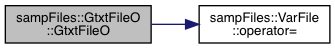
\includegraphics[width=323pt]{classsamp_files_1_1_gtxt_file_o_a84944d8c2b0e6c6eeb877b53e17fc104_cgraph}
\end{center}
\end{figure}


The documentation for this class was generated from the following files\+:\begin{DoxyCompactItemize}
\item 
\hyperlink{varfiles_8hpp}{varfiles.\+hpp}\item 
\hyperlink{varfiles_8cpp}{varfiles.\+cpp}\end{DoxyCompactItemize}

\hypertarget{classsamp_files_1_1_hmp_file}{}\section{samp\+Files\+:\+:Hmp\+File Class Reference}
\label{classsamp_files_1_1_hmp_file}\index{samp\+Files\+::\+Hmp\+File@{samp\+Files\+::\+Hmp\+File}}


Hapmap (H\+MP) file base class.  




{\ttfamily \#include $<$varfiles.\+hpp$>$}



Inheritance diagram for samp\+Files\+:\+:Hmp\+File\+:\nopagebreak
\begin{figure}[H]
\begin{center}
\leavevmode
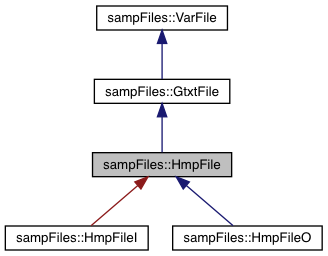
\includegraphics[width=318pt]{classsamp_files_1_1_hmp_file__inherit__graph}
\end{center}
\end{figure}


Collaboration diagram for samp\+Files\+:\+:Hmp\+File\+:\nopagebreak
\begin{figure}[H]
\begin{center}
\leavevmode
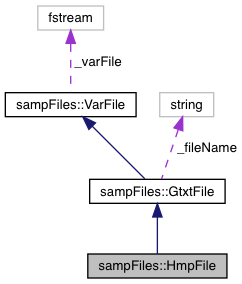
\includegraphics[width=254pt]{classsamp_files_1_1_hmp_file__coll__graph}
\end{center}
\end{figure}
\subsection*{Public Member Functions}
\begin{DoxyCompactItemize}
\item 
\mbox{\Hypertarget{classsamp_files_1_1_hmp_file_a12005328f7ce0f31615cb4765602ce4e}\label{classsamp_files_1_1_hmp_file_a12005328f7ce0f31615cb4765602ce4e}} 
\hyperlink{classsamp_files_1_1_hmp_file_a12005328f7ce0f31615cb4765602ce4e}{Hmp\+File} ()
\begin{DoxyCompactList}\small\item\em Default constructor. \end{DoxyCompactList}\item 
\hyperlink{classsamp_files_1_1_hmp_file_a69e670927eea527587417d28e05734cd}{Hmp\+File} (const string \&file\+Name)
\begin{DoxyCompactList}\small\item\em Constructor with file name. \end{DoxyCompactList}\item 
\mbox{\Hypertarget{classsamp_files_1_1_hmp_file_a1b4d1f28f04e5dbd2a6f81008171b9c0}\label{classsamp_files_1_1_hmp_file_a1b4d1f28f04e5dbd2a6f81008171b9c0}} 
\hyperlink{classsamp_files_1_1_hmp_file_a1b4d1f28f04e5dbd2a6f81008171b9c0}{Hmp\+File} (const \hyperlink{classsamp_files_1_1_hmp_file}{Hmp\+File} \&in)=default
\begin{DoxyCompactList}\small\item\em Copy constructor. \end{DoxyCompactList}\item 
\mbox{\Hypertarget{classsamp_files_1_1_hmp_file_a338d25389296d566b2efd06335ee61fe}\label{classsamp_files_1_1_hmp_file_a338d25389296d566b2efd06335ee61fe}} 
\hyperlink{classsamp_files_1_1_hmp_file}{Hmp\+File} \& \hyperlink{classsamp_files_1_1_hmp_file_a338d25389296d566b2efd06335ee61fe}{operator=} (const \hyperlink{classsamp_files_1_1_hmp_file}{Hmp\+File} \&in)=default
\begin{DoxyCompactList}\small\item\em Copy assignment. \end{DoxyCompactList}\item 
\mbox{\Hypertarget{classsamp_files_1_1_hmp_file_a1344bb70d7a2db7cb44eb1cc0e5d565e}\label{classsamp_files_1_1_hmp_file_a1344bb70d7a2db7cb44eb1cc0e5d565e}} 
\hyperlink{classsamp_files_1_1_hmp_file_a1344bb70d7a2db7cb44eb1cc0e5d565e}{Hmp\+File} (\hyperlink{classsamp_files_1_1_hmp_file}{Hmp\+File} \&\&in)=default
\begin{DoxyCompactList}\small\item\em Move constructor. \end{DoxyCompactList}\item 
\mbox{\Hypertarget{classsamp_files_1_1_hmp_file_a24bc4890a428b7e6d7530795dd3b4480}\label{classsamp_files_1_1_hmp_file_a24bc4890a428b7e6d7530795dd3b4480}} 
\hyperlink{classsamp_files_1_1_hmp_file}{Hmp\+File} \& \hyperlink{classsamp_files_1_1_hmp_file_a24bc4890a428b7e6d7530795dd3b4480}{operator=} (\hyperlink{classsamp_files_1_1_hmp_file}{Hmp\+File} \&\&in)=default
\begin{DoxyCompactList}\small\item\em Move assignment. \end{DoxyCompactList}\item 
\mbox{\Hypertarget{classsamp_files_1_1_hmp_file_a44354598fd14540e5b2775262e828318}\label{classsamp_files_1_1_hmp_file_a44354598fd14540e5b2775262e828318}} 
\hyperlink{classsamp_files_1_1_hmp_file_a44354598fd14540e5b2775262e828318}{$\sim$\+Hmp\+File} ()
\begin{DoxyCompactList}\small\item\em Destructor. \end{DoxyCompactList}\item 
\mbox{\Hypertarget{classsamp_files_1_1_hmp_file_a9bd150295e4b261af45b78c19547a593}\label{classsamp_files_1_1_hmp_file_a9bd150295e4b261af45b78c19547a593}} 
virtual void \hyperlink{classsamp_files_1_1_hmp_file_a9bd150295e4b261af45b78c19547a593}{open} ()
\begin{DoxyCompactList}\small\item\em Open stream (does nothing) \end{DoxyCompactList}\item 
\mbox{\Hypertarget{classsamp_files_1_1_hmp_file_a72b0f031c2260be66397752be52c929f}\label{classsamp_files_1_1_hmp_file_a72b0f031c2260be66397752be52c929f}} 
virtual void \hyperlink{classsamp_files_1_1_hmp_file_a72b0f031c2260be66397752be52c929f}{close} ()
\begin{DoxyCompactList}\small\item\em Close stream. \end{DoxyCompactList}\end{DoxyCompactItemize}
\subsection*{Additional Inherited Members}


\subsection{Detailed Description}
Hapmap (H\+MP) file base class. 

Sets up streams for H\+MP files. 

\subsection{Constructor \& Destructor Documentation}
\mbox{\Hypertarget{classsamp_files_1_1_hmp_file_a69e670927eea527587417d28e05734cd}\label{classsamp_files_1_1_hmp_file_a69e670927eea527587417d28e05734cd}} 
\index{samp\+Files\+::\+Hmp\+File@{samp\+Files\+::\+Hmp\+File}!Hmp\+File@{Hmp\+File}}
\index{Hmp\+File@{Hmp\+File}!samp\+Files\+::\+Hmp\+File@{samp\+Files\+::\+Hmp\+File}}
\subsubsection{\texorpdfstring{Hmp\+File()}{HmpFile()}}
{\footnotesize\ttfamily samp\+Files\+::\+Hmp\+File\+::\+Hmp\+File (\begin{DoxyParamCaption}\item[{const string \&}]{file\+Name }\end{DoxyParamCaption})\hspace{0.3cm}{\ttfamily [inline]}}



Constructor with file name. 


\begin{DoxyParams}[1]{Parameters}
\mbox{\tt in}  & {\em file\+Name} & file name \\
\hline
\end{DoxyParams}
Here is the call graph for this function\+:\nopagebreak
\begin{figure}[H]
\begin{center}
\leavevmode
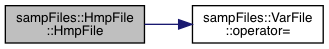
\includegraphics[width=318pt]{classsamp_files_1_1_hmp_file_a69e670927eea527587417d28e05734cd_cgraph}
\end{center}
\end{figure}


The documentation for this class was generated from the following files\+:\begin{DoxyCompactItemize}
\item 
\hyperlink{varfiles_8hpp}{varfiles.\+hpp}\item 
\hyperlink{varfiles_8cpp}{varfiles.\+cpp}\end{DoxyCompactItemize}

\hypertarget{classsamp_files_1_1_hmp_file_i}{}\section{samp\+Files\+:\+:Hmp\+FileI Class Reference}
\label{classsamp_files_1_1_hmp_file_i}\index{samp\+Files\+::\+Hmp\+FileI@{samp\+Files\+::\+Hmp\+FileI}}


H\+MP file input class.  




{\ttfamily \#include $<$varfiles.\+hpp$>$}



Inheritance diagram for samp\+Files\+:\+:Hmp\+FileI\+:\nopagebreak
\begin{figure}[H]
\begin{center}
\leavevmode
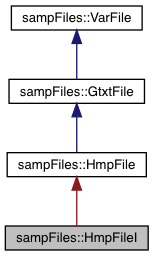
\includegraphics[width=187pt]{classsamp_files_1_1_hmp_file_i__inherit__graph}
\end{center}
\end{figure}


Collaboration diagram for samp\+Files\+:\+:Hmp\+FileI\+:\nopagebreak
\begin{figure}[H]
\begin{center}
\leavevmode
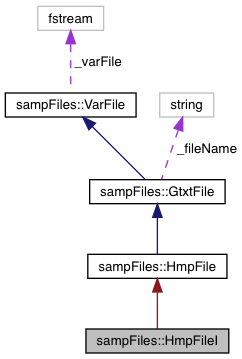
\includegraphics[width=254pt]{classsamp_files_1_1_hmp_file_i__coll__graph}
\end{center}
\end{figure}
\subsection*{Public Member Functions}
\begin{DoxyCompactItemize}
\item 
\mbox{\Hypertarget{classsamp_files_1_1_hmp_file_i_afca3094a6302e44a9a209a33ce0883ec}\label{classsamp_files_1_1_hmp_file_i_afca3094a6302e44a9a209a33ce0883ec}} 
\hyperlink{classsamp_files_1_1_hmp_file_i_afca3094a6302e44a9a209a33ce0883ec}{Hmp\+FileI} ()
\begin{DoxyCompactList}\small\item\em Default constructor. \end{DoxyCompactList}\item 
\hyperlink{classsamp_files_1_1_hmp_file_i_a61a3b829ed54c8c7e6431747a20f4466}{Hmp\+FileI} (const string \&file\+Name)
\begin{DoxyCompactList}\small\item\em File name constructor. \end{DoxyCompactList}\item 
\mbox{\Hypertarget{classsamp_files_1_1_hmp_file_i_a9989724aefaeea5520af821a1e3732a7}\label{classsamp_files_1_1_hmp_file_i_a9989724aefaeea5520af821a1e3732a7}} 
\hyperlink{classsamp_files_1_1_hmp_file_i_a9989724aefaeea5520af821a1e3732a7}{Hmp\+FileI} (const \hyperlink{classsamp_files_1_1_hmp_file_i}{Hmp\+FileI} \&in)=default
\begin{DoxyCompactList}\small\item\em Copy constructor. \end{DoxyCompactList}\item 
\mbox{\Hypertarget{classsamp_files_1_1_hmp_file_i_a1e26ee01a8c7a7a5a1b55656f41cee0d}\label{classsamp_files_1_1_hmp_file_i_a1e26ee01a8c7a7a5a1b55656f41cee0d}} 
\hyperlink{classsamp_files_1_1_hmp_file_i}{Hmp\+FileI} \& \hyperlink{classsamp_files_1_1_hmp_file_i_a1e26ee01a8c7a7a5a1b55656f41cee0d}{operator=} (const \hyperlink{classsamp_files_1_1_hmp_file_i}{Hmp\+FileI} \&in)=default
\begin{DoxyCompactList}\small\item\em Copy assignment. \end{DoxyCompactList}\item 
\mbox{\Hypertarget{classsamp_files_1_1_hmp_file_i_a7f1fa0e7336f551e3867780d91d99519}\label{classsamp_files_1_1_hmp_file_i_a7f1fa0e7336f551e3867780d91d99519}} 
\hyperlink{classsamp_files_1_1_hmp_file_i_a7f1fa0e7336f551e3867780d91d99519}{Hmp\+FileI} (\hyperlink{classsamp_files_1_1_hmp_file_i}{Hmp\+FileI} \&\&in)=default
\begin{DoxyCompactList}\small\item\em Move constructor. \end{DoxyCompactList}\item 
\mbox{\Hypertarget{classsamp_files_1_1_hmp_file_i_abb726792996c45a55ab741296f39a875}\label{classsamp_files_1_1_hmp_file_i_abb726792996c45a55ab741296f39a875}} 
\hyperlink{classsamp_files_1_1_hmp_file_i}{Hmp\+FileI} \& \hyperlink{classsamp_files_1_1_hmp_file_i_abb726792996c45a55ab741296f39a875}{operator=} (\hyperlink{classsamp_files_1_1_hmp_file_i}{Hmp\+FileI} \&\&in)=default
\begin{DoxyCompactList}\small\item\em Move assignment. \end{DoxyCompactList}\item 
\mbox{\Hypertarget{classsamp_files_1_1_hmp_file_i_aa8fd3c3e48c2efc2c45f38be30be66a1}\label{classsamp_files_1_1_hmp_file_i_aa8fd3c3e48c2efc2c45f38be30be66a1}} 
\hyperlink{classsamp_files_1_1_hmp_file_i_aa8fd3c3e48c2efc2c45f38be30be66a1}{$\sim$\+Hmp\+FileI} ()
\begin{DoxyCompactList}\small\item\em Destructor. \end{DoxyCompactList}\item 
\mbox{\Hypertarget{classsamp_files_1_1_hmp_file_i_a6bf4de03c605ed70d74766c94f1e12ae}\label{classsamp_files_1_1_hmp_file_i_a6bf4de03c605ed70d74766c94f1e12ae}} 
void \hyperlink{classsamp_files_1_1_hmp_file_i_a6bf4de03c605ed70d74766c94f1e12ae}{open} ()
\begin{DoxyCompactList}\small\item\em Open stream to read. \end{DoxyCompactList}\item 
void \hyperlink{classsamp_files_1_1_hmp_file_i_afd02563de7ecb89a94e8af4110676710}{sample} (\hyperlink{classsamp_files_1_1_hmp_file_o}{Hmp\+FileO} \&out, const uint64\+\_\+t \&n)
\begin{DoxyCompactList}\small\item\em Sample S\+N\+Ps and save to H\+MP file. \end{DoxyCompactList}\item 
\mbox{\Hypertarget{classsamp_files_1_1_hmp_file_i_a1439d1c790c82a8c3c5634d65fc99606}\label{classsamp_files_1_1_hmp_file_i_a1439d1c790c82a8c3c5634d65fc99606}} 
uint64\+\_\+t \hyperlink{classsamp_files_1_1_hmp_file_i_a1439d1c790c82a8c3c5634d65fc99606}{nsnp} ()
\begin{DoxyCompactList}\small\item\em Number of S\+N\+Ps in the object. \end{DoxyCompactList}\end{DoxyCompactItemize}
\subsection*{Protected Member Functions}
\begin{DoxyCompactItemize}
\item 
uint64\+\_\+t \hyperlink{classsamp_files_1_1_hmp_file_i_a2a39e46be7d94f39a4c6250855c1da1c}{\+\_\+num\+Lines} ()
\begin{DoxyCompactList}\small\item\em Get number of S\+N\+Ps in the H\+MP file. \end{DoxyCompactList}\end{DoxyCompactItemize}


\subsection{Detailed Description}
H\+MP file input class. 

Reads H\+MP files, skipping or copying the header as necessary. 

\subsection{Constructor \& Destructor Documentation}
\mbox{\Hypertarget{classsamp_files_1_1_hmp_file_i_a61a3b829ed54c8c7e6431747a20f4466}\label{classsamp_files_1_1_hmp_file_i_a61a3b829ed54c8c7e6431747a20f4466}} 
\index{samp\+Files\+::\+Hmp\+FileI@{samp\+Files\+::\+Hmp\+FileI}!Hmp\+FileI@{Hmp\+FileI}}
\index{Hmp\+FileI@{Hmp\+FileI}!samp\+Files\+::\+Hmp\+FileI@{samp\+Files\+::\+Hmp\+FileI}}
\subsubsection{\texorpdfstring{Hmp\+File\+I()}{HmpFileI()}}
{\footnotesize\ttfamily Hmp\+File\+I\+::\+Hmp\+FileI (\begin{DoxyParamCaption}\item[{const string \&}]{file\+Name }\end{DoxyParamCaption})}



File name constructor. 


\begin{DoxyParams}[1]{Parameters}
\mbox{\tt in}  & {\em file\+Name} & file name including extension \\
\hline
\end{DoxyParams}


\subsection{Member Function Documentation}
\mbox{\Hypertarget{classsamp_files_1_1_hmp_file_i_a2a39e46be7d94f39a4c6250855c1da1c}\label{classsamp_files_1_1_hmp_file_i_a2a39e46be7d94f39a4c6250855c1da1c}} 
\index{samp\+Files\+::\+Hmp\+FileI@{samp\+Files\+::\+Hmp\+FileI}!\+\_\+num\+Lines@{\+\_\+num\+Lines}}
\index{\+\_\+num\+Lines@{\+\_\+num\+Lines}!samp\+Files\+::\+Hmp\+FileI@{samp\+Files\+::\+Hmp\+FileI}}
\subsubsection{\texorpdfstring{\+\_\+num\+Lines()}{\_numLines()}}
{\footnotesize\ttfamily uint64\+\_\+t Hmp\+File\+I\+::\+\_\+num\+Lines (\begin{DoxyParamCaption}{ }\end{DoxyParamCaption})\hspace{0.3cm}{\ttfamily [protected]}}



Get number of S\+N\+Ps in the H\+MP file. 

Assumes Unix-\/like line endings. Header is not counted.

\begin{DoxyReturn}{Returns}
number of S\+N\+Ps 
\end{DoxyReturn}
Here is the caller graph for this function\+:\nopagebreak
\begin{figure}[H]
\begin{center}
\leavevmode
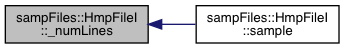
\includegraphics[width=330pt]{classsamp_files_1_1_hmp_file_i_a2a39e46be7d94f39a4c6250855c1da1c_icgraph}
\end{center}
\end{figure}
\mbox{\Hypertarget{classsamp_files_1_1_hmp_file_i_afd02563de7ecb89a94e8af4110676710}\label{classsamp_files_1_1_hmp_file_i_afd02563de7ecb89a94e8af4110676710}} 
\index{samp\+Files\+::\+Hmp\+FileI@{samp\+Files\+::\+Hmp\+FileI}!sample@{sample}}
\index{sample@{sample}!samp\+Files\+::\+Hmp\+FileI@{samp\+Files\+::\+Hmp\+FileI}}
\subsubsection{\texorpdfstring{sample()}{sample()}}
{\footnotesize\ttfamily void Hmp\+File\+I\+::sample (\begin{DoxyParamCaption}\item[{\hyperlink{classsamp_files_1_1_hmp_file_o}{Hmp\+FileO} \&}]{out,  }\item[{const uint64\+\_\+t \&}]{n }\end{DoxyParamCaption})}



Sample S\+N\+Ps and save to H\+MP file. 

Sample $n$ S\+N\+Ps without replacement from the file represented by the current object and save to the {\ttfamily out} object. Uses Vitter\textquotesingle{}s \cite{vitter87a} method. Number of samples has to be smaller that the number of S\+N\+Ps in the file.


\begin{DoxyParams}[1]{Parameters}
\mbox{\tt in}  & {\em out} & output object \\
\hline
\mbox{\tt in}  & {\em n} & number of S\+N\+Ps to sample \\
\hline
\end{DoxyParams}
Here is the call graph for this function\+:\nopagebreak
\begin{figure}[H]
\begin{center}
\leavevmode
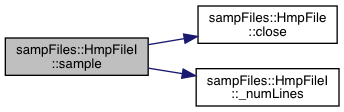
\includegraphics[width=330pt]{classsamp_files_1_1_hmp_file_i_afd02563de7ecb89a94e8af4110676710_cgraph}
\end{center}
\end{figure}


The documentation for this class was generated from the following files\+:\begin{DoxyCompactItemize}
\item 
\hyperlink{varfiles_8hpp}{varfiles.\+hpp}\item 
\hyperlink{varfiles_8cpp}{varfiles.\+cpp}\end{DoxyCompactItemize}

\hypertarget{classsamp_files_1_1_hmp_file_o}{}\section{samp\+Files\+:\+:Hmp\+FileO Class Reference}
\label{classsamp_files_1_1_hmp_file_o}\index{samp\+Files\+::\+Hmp\+FileO@{samp\+Files\+::\+Hmp\+FileO}}


H\+MP file output class.  




{\ttfamily \#include $<$varfiles.\+hpp$>$}



Inheritance diagram for samp\+Files\+:\+:Hmp\+FileO\+:\nopagebreak
\begin{figure}[H]
\begin{center}
\leavevmode
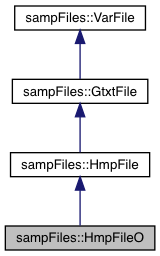
\includegraphics[width=192pt]{classsamp_files_1_1_hmp_file_o__inherit__graph}
\end{center}
\end{figure}


Collaboration diagram for samp\+Files\+:\+:Hmp\+FileO\+:\nopagebreak
\begin{figure}[H]
\begin{center}
\leavevmode
\includegraphics[width=254pt]{classsamp_files_1_1_hmp_file_o__coll__graph}
\end{center}
\end{figure}
\subsection*{Public Member Functions}
\begin{DoxyCompactItemize}
\item 
\mbox{\Hypertarget{classsamp_files_1_1_hmp_file_o_a1e9b87d83403ac88fc508505d9951afd}\label{classsamp_files_1_1_hmp_file_o_a1e9b87d83403ac88fc508505d9951afd}} 
\hyperlink{classsamp_files_1_1_hmp_file_o_a1e9b87d83403ac88fc508505d9951afd}{Hmp\+FileO} ()
\begin{DoxyCompactList}\small\item\em Default constructor. \end{DoxyCompactList}\item 
\hyperlink{classsamp_files_1_1_hmp_file_o_af360694580dc1cf427b0b59375f0751f}{Hmp\+FileO} (const string \&file\+Name)
\begin{DoxyCompactList}\small\item\em File name constructor. \end{DoxyCompactList}\item 
\mbox{\Hypertarget{classsamp_files_1_1_hmp_file_o_a11b3596fbf8f79d3b34a01e959cdde46}\label{classsamp_files_1_1_hmp_file_o_a11b3596fbf8f79d3b34a01e959cdde46}} 
\hyperlink{classsamp_files_1_1_hmp_file_o_a11b3596fbf8f79d3b34a01e959cdde46}{Hmp\+FileO} (const \hyperlink{classsamp_files_1_1_hmp_file_o}{Hmp\+FileO} \&in)=default
\begin{DoxyCompactList}\small\item\em Copy constructor. \end{DoxyCompactList}\item 
\mbox{\Hypertarget{classsamp_files_1_1_hmp_file_o_a2dae478003580d4ef3e7437618ad1b8e}\label{classsamp_files_1_1_hmp_file_o_a2dae478003580d4ef3e7437618ad1b8e}} 
\hyperlink{classsamp_files_1_1_hmp_file_o}{Hmp\+FileO} \& \hyperlink{classsamp_files_1_1_hmp_file_o_a2dae478003580d4ef3e7437618ad1b8e}{operator=} (const \hyperlink{classsamp_files_1_1_hmp_file_o}{Hmp\+FileO} \&in)=default
\begin{DoxyCompactList}\small\item\em Copy assignment. \end{DoxyCompactList}\item 
\mbox{\Hypertarget{classsamp_files_1_1_hmp_file_o_acc71624d6213ede99b688a5a32b52111}\label{classsamp_files_1_1_hmp_file_o_acc71624d6213ede99b688a5a32b52111}} 
\hyperlink{classsamp_files_1_1_hmp_file_o_acc71624d6213ede99b688a5a32b52111}{Hmp\+FileO} (\hyperlink{classsamp_files_1_1_hmp_file_o}{Hmp\+FileO} \&\&in)=default
\begin{DoxyCompactList}\small\item\em Move constructor. \end{DoxyCompactList}\item 
\mbox{\Hypertarget{classsamp_files_1_1_hmp_file_o_a02160aa511bfbace0f6fdc5074eb2ac6}\label{classsamp_files_1_1_hmp_file_o_a02160aa511bfbace0f6fdc5074eb2ac6}} 
\hyperlink{classsamp_files_1_1_hmp_file_o}{Hmp\+FileO} \& \hyperlink{classsamp_files_1_1_hmp_file_o_a02160aa511bfbace0f6fdc5074eb2ac6}{operator=} (\hyperlink{classsamp_files_1_1_hmp_file_o}{Hmp\+FileO} \&\&in)=default
\begin{DoxyCompactList}\small\item\em Move assignment. \end{DoxyCompactList}\item 
\mbox{\Hypertarget{classsamp_files_1_1_hmp_file_o_a54b7bd87bd30499b2e60b360a12bc4e2}\label{classsamp_files_1_1_hmp_file_o_a54b7bd87bd30499b2e60b360a12bc4e2}} 
\hyperlink{classsamp_files_1_1_hmp_file_o_a54b7bd87bd30499b2e60b360a12bc4e2}{$\sim$\+Hmp\+FileO} ()
\begin{DoxyCompactList}\small\item\em Destructor. \end{DoxyCompactList}\item 
\mbox{\Hypertarget{classsamp_files_1_1_hmp_file_o_a0d49862be8b4065b99e2795a91fb01b6}\label{classsamp_files_1_1_hmp_file_o_a0d49862be8b4065b99e2795a91fb01b6}} 
void \hyperlink{classsamp_files_1_1_hmp_file_o_a0d49862be8b4065b99e2795a91fb01b6}{open} ()
\begin{DoxyCompactList}\small\item\em Open stream to write. \end{DoxyCompactList}\end{DoxyCompactItemize}
\subsection*{Friends}
\begin{DoxyCompactItemize}
\item 
\mbox{\Hypertarget{classsamp_files_1_1_hmp_file_o_a1562cc41c56f46e4090775304e4cdfcd}\label{classsamp_files_1_1_hmp_file_o_a1562cc41c56f46e4090775304e4cdfcd}} 
class {\bfseries Hmp\+FileI}
\end{DoxyCompactItemize}
\subsection*{Additional Inherited Members}


\subsection{Detailed Description}
H\+MP file output class. 

Writes H\+MP files. 

\subsection{Constructor \& Destructor Documentation}
\mbox{\Hypertarget{classsamp_files_1_1_hmp_file_o_af360694580dc1cf427b0b59375f0751f}\label{classsamp_files_1_1_hmp_file_o_af360694580dc1cf427b0b59375f0751f}} 
\index{samp\+Files\+::\+Hmp\+FileO@{samp\+Files\+::\+Hmp\+FileO}!Hmp\+FileO@{Hmp\+FileO}}
\index{Hmp\+FileO@{Hmp\+FileO}!samp\+Files\+::\+Hmp\+FileO@{samp\+Files\+::\+Hmp\+FileO}}
\subsubsection{\texorpdfstring{Hmp\+File\+O()}{HmpFileO()}}
{\footnotesize\ttfamily samp\+Files\+::\+Hmp\+File\+O\+::\+Hmp\+FileO (\begin{DoxyParamCaption}\item[{const string \&}]{file\+Name }\end{DoxyParamCaption})\hspace{0.3cm}{\ttfamily [inline]}}



File name constructor. 


\begin{DoxyParams}[1]{Parameters}
\mbox{\tt in}  & {\em file\+Name} & file name including the extension \\
\hline
\end{DoxyParams}
Here is the call graph for this function\+:\nopagebreak
\begin{figure}[H]
\begin{center}
\leavevmode
\includegraphics[width=326pt]{classsamp_files_1_1_hmp_file_o_af360694580dc1cf427b0b59375f0751f_cgraph}
\end{center}
\end{figure}


The documentation for this class was generated from the following files\+:\begin{DoxyCompactItemize}
\item 
\hyperlink{varfiles_8hpp}{varfiles.\+hpp}\item 
\hyperlink{varfiles_8cpp}{varfiles.\+cpp}\end{DoxyCompactItemize}

\hypertarget{classsamp_files_1_1_pop_index}{}\section{samp\+Files\+:\+:Pop\+Index Class Reference}
\label{classsamp_files_1_1_pop_index}\index{samp\+Files\+::\+Pop\+Index@{samp\+Files\+::\+Pop\+Index}}


Population index.  




{\ttfamily \#include $<$populations.\+hpp$>$}

\subsection*{Public Member Functions}
\begin{DoxyCompactItemize}
\item 
\mbox{\Hypertarget{classsamp_files_1_1_pop_index_a4490c400619ba5725c6e14bfb5bcc069}\label{classsamp_files_1_1_pop_index_a4490c400619ba5725c6e14bfb5bcc069}} 
\hyperlink{classsamp_files_1_1_pop_index_a4490c400619ba5725c6e14bfb5bcc069}{Pop\+Index} ()
\begin{DoxyCompactList}\small\item\em Default constructor. \end{DoxyCompactList}\item 
\hyperlink{classsamp_files_1_1_pop_index_a27367217cfb5f85abda425baa1d755b9}{Pop\+Index} (const int $\ast$arr, const size\+\_\+t \&N)
\begin{DoxyCompactList}\small\item\em Array constructor. \end{DoxyCompactList}\item 
\hyperlink{classsamp_files_1_1_pop_index_aaf4cec726d9befe823c7d6ff4d36d5ce}{Pop\+Index} (const string \&in\+File\+Name)
\begin{DoxyCompactList}\small\item\em File read constructor. \end{DoxyCompactList}\item 
vector$<$ size\+\_\+t $>$ \& \hyperlink{classsamp_files_1_1_pop_index_ad3e3ff5964bea3b17bf54c2fc3af231c}{operator\mbox{[}$\,$\mbox{]}} (const size\+\_\+t \&i)
\begin{DoxyCompactList}\small\item\em Vector subscript operator. \end{DoxyCompactList}\item 
const vector$<$ size\+\_\+t $>$ \& \hyperlink{classsamp_files_1_1_pop_index_a56dea775828fc2a6b8b5b110429f67a5}{operator\mbox{[}$\,$\mbox{]}} (const size\+\_\+t \&i) const
\begin{DoxyCompactList}\small\item\em {\ttfamily const} vector subscript operator \end{DoxyCompactList}\item 
size\+\_\+t \hyperlink{classsamp_files_1_1_pop_index_a5a58b623938c025a287711de86a4021a}{pop\+Size} (const size\+\_\+t \&i)
\begin{DoxyCompactList}\small\item\em Population size. \end{DoxyCompactList}\item 
size\+\_\+t \hyperlink{classsamp_files_1_1_pop_index_aef299f007e2123b430d6d36fa50d4d16}{pop\+Size} (const size\+\_\+t \&i) const
\begin{DoxyCompactList}\small\item\em {\ttfamily const} population size \end{DoxyCompactList}\item 
size\+\_\+t \hyperlink{classsamp_files_1_1_pop_index_a1de6bf81252ebc9d7d2521f62487b042}{size} ()
\begin{DoxyCompactList}\small\item\em Total sample size. \end{DoxyCompactList}\item 
size\+\_\+t \hyperlink{classsamp_files_1_1_pop_index_a251a3004894d15691b6f12adb84b0ad5}{size} () const
\begin{DoxyCompactList}\small\item\em {\ttfamily const} total sample size \end{DoxyCompactList}\item 
size\+\_\+t \hyperlink{classsamp_files_1_1_pop_index_ae478775b725c4cbae2be5b136c6e6856}{pop\+Number} ()
\begin{DoxyCompactList}\small\item\em Number of populations. \end{DoxyCompactList}\item 
size\+\_\+t \hyperlink{classsamp_files_1_1_pop_index_a6dde50396274681751d41b058af376d7}{pop\+Number} () const
\begin{DoxyCompactList}\small\item\em {\ttfamily const} number of populations \end{DoxyCompactList}\end{DoxyCompactItemize}


\subsection{Detailed Description}
Population index. 

For each population, contains indexes of the lines that belong to it. 

\subsection{Constructor \& Destructor Documentation}
\mbox{\Hypertarget{classsamp_files_1_1_pop_index_a27367217cfb5f85abda425baa1d755b9}\label{classsamp_files_1_1_pop_index_a27367217cfb5f85abda425baa1d755b9}} 
\index{samp\+Files\+::\+Pop\+Index@{samp\+Files\+::\+Pop\+Index}!Pop\+Index@{Pop\+Index}}
\index{Pop\+Index@{Pop\+Index}!samp\+Files\+::\+Pop\+Index@{samp\+Files\+::\+Pop\+Index}}
\subsubsection{\texorpdfstring{Pop\+Index()}{PopIndex()}\hspace{0.1cm}{\footnotesize\ttfamily [1/2]}}
{\footnotesize\ttfamily Pop\+Index\+::\+Pop\+Index (\begin{DoxyParamCaption}\item[{const int $\ast$}]{arr,  }\item[{const size\+\_\+t \&}]{N }\end{DoxyParamCaption})}



Array constructor. 

The input array has an element for each line, and the value of that element is the population ID in the form of an {\itshape int} that is base-\/1 (i.\+e., if line N is in the first population, then {\ttfamily arr\mbox{[}N\mbox{]} == 1}).


\begin{DoxyParams}[1]{Parameters}
\mbox{\tt in}  & {\em arr} & array of population I\+Ds \\
\hline
\mbox{\tt in}  & {\em N} & array length \\
\hline
\end{DoxyParams}
\mbox{\Hypertarget{classsamp_files_1_1_pop_index_aaf4cec726d9befe823c7d6ff4d36d5ce}\label{classsamp_files_1_1_pop_index_aaf4cec726d9befe823c7d6ff4d36d5ce}} 
\index{samp\+Files\+::\+Pop\+Index@{samp\+Files\+::\+Pop\+Index}!Pop\+Index@{Pop\+Index}}
\index{Pop\+Index@{Pop\+Index}!samp\+Files\+::\+Pop\+Index@{samp\+Files\+::\+Pop\+Index}}
\subsubsection{\texorpdfstring{Pop\+Index()}{PopIndex()}\hspace{0.1cm}{\footnotesize\ttfamily [2/2]}}
{\footnotesize\ttfamily Pop\+Index\+::\+Pop\+Index (\begin{DoxyParamCaption}\item[{const string \&}]{in\+File\+Name }\end{DoxyParamCaption})}



File read constructor. 

The input file has an entry for each line (separated by white space), and the value of that entry is the population ID in the form of an {\itshape int} that is base-\/1 (i.\+e., if line N is in the first population, then {\ttfamily arr\mbox{[}N\mbox{]} == 1}).


\begin{DoxyParams}[1]{Parameters}
\mbox{\tt in}  & {\em in\+File\+Name} & input file name \\
\hline
\end{DoxyParams}


\subsection{Member Function Documentation}
\mbox{\Hypertarget{classsamp_files_1_1_pop_index_ad3e3ff5964bea3b17bf54c2fc3af231c}\label{classsamp_files_1_1_pop_index_ad3e3ff5964bea3b17bf54c2fc3af231c}} 
\index{samp\+Files\+::\+Pop\+Index@{samp\+Files\+::\+Pop\+Index}!operator\mbox{[}\mbox{]}@{operator[]}}
\index{operator\mbox{[}\mbox{]}@{operator[]}!samp\+Files\+::\+Pop\+Index@{samp\+Files\+::\+Pop\+Index}}
\subsubsection{\texorpdfstring{operator[]()}{operator[]()}\hspace{0.1cm}{\footnotesize\ttfamily [1/2]}}
{\footnotesize\ttfamily vector$<$size\+\_\+t$>$\& samp\+Files\+::\+Pop\+Index\+::operator\mbox{[}$\,$\mbox{]} (\begin{DoxyParamCaption}\item[{const size\+\_\+t \&}]{i }\end{DoxyParamCaption})\hspace{0.3cm}{\ttfamily [inline]}}



Vector subscript operator. 

Returns the index of population {\itshape i}.


\begin{DoxyParams}[1]{Parameters}
\mbox{\tt in}  & {\em i} & population index \\
\hline
\end{DoxyParams}
\begin{DoxyReturn}{Returns}
index of line I\+Ds 
\end{DoxyReturn}
\mbox{\Hypertarget{classsamp_files_1_1_pop_index_a56dea775828fc2a6b8b5b110429f67a5}\label{classsamp_files_1_1_pop_index_a56dea775828fc2a6b8b5b110429f67a5}} 
\index{samp\+Files\+::\+Pop\+Index@{samp\+Files\+::\+Pop\+Index}!operator\mbox{[}\mbox{]}@{operator[]}}
\index{operator\mbox{[}\mbox{]}@{operator[]}!samp\+Files\+::\+Pop\+Index@{samp\+Files\+::\+Pop\+Index}}
\subsubsection{\texorpdfstring{operator[]()}{operator[]()}\hspace{0.1cm}{\footnotesize\ttfamily [2/2]}}
{\footnotesize\ttfamily const vector$<$size\+\_\+t$>$\& samp\+Files\+::\+Pop\+Index\+::operator\mbox{[}$\,$\mbox{]} (\begin{DoxyParamCaption}\item[{const size\+\_\+t \&}]{i }\end{DoxyParamCaption}) const\hspace{0.3cm}{\ttfamily [inline]}}



{\ttfamily const} vector subscript operator 

Returns the index of population {\itshape i}.


\begin{DoxyParams}[1]{Parameters}
\mbox{\tt in}  & {\em i} & population index \\
\hline
\end{DoxyParams}
\begin{DoxyReturn}{Returns}
index of line I\+Ds 
\end{DoxyReturn}
\mbox{\Hypertarget{classsamp_files_1_1_pop_index_ae478775b725c4cbae2be5b136c6e6856}\label{classsamp_files_1_1_pop_index_ae478775b725c4cbae2be5b136c6e6856}} 
\index{samp\+Files\+::\+Pop\+Index@{samp\+Files\+::\+Pop\+Index}!pop\+Number@{pop\+Number}}
\index{pop\+Number@{pop\+Number}!samp\+Files\+::\+Pop\+Index@{samp\+Files\+::\+Pop\+Index}}
\subsubsection{\texorpdfstring{pop\+Number()}{popNumber()}\hspace{0.1cm}{\footnotesize\ttfamily [1/2]}}
{\footnotesize\ttfamily size\+\_\+t samp\+Files\+::\+Pop\+Index\+::pop\+Number (\begin{DoxyParamCaption}{ }\end{DoxyParamCaption})\hspace{0.3cm}{\ttfamily [inline]}}



Number of populations. 

\begin{DoxyReturn}{Returns}
number of populations 
\end{DoxyReturn}
Here is the caller graph for this function\+:\nopagebreak
\begin{figure}[H]
\begin{center}
\leavevmode
\includegraphics[width=348pt]{classsamp_files_1_1_pop_index_ae478775b725c4cbae2be5b136c6e6856_icgraph}
\end{center}
\end{figure}
\mbox{\Hypertarget{classsamp_files_1_1_pop_index_a6dde50396274681751d41b058af376d7}\label{classsamp_files_1_1_pop_index_a6dde50396274681751d41b058af376d7}} 
\index{samp\+Files\+::\+Pop\+Index@{samp\+Files\+::\+Pop\+Index}!pop\+Number@{pop\+Number}}
\index{pop\+Number@{pop\+Number}!samp\+Files\+::\+Pop\+Index@{samp\+Files\+::\+Pop\+Index}}
\subsubsection{\texorpdfstring{pop\+Number()}{popNumber()}\hspace{0.1cm}{\footnotesize\ttfamily [2/2]}}
{\footnotesize\ttfamily size\+\_\+t samp\+Files\+::\+Pop\+Index\+::pop\+Number (\begin{DoxyParamCaption}{ }\end{DoxyParamCaption}) const\hspace{0.3cm}{\ttfamily [inline]}}



{\ttfamily const} number of populations 

\begin{DoxyReturn}{Returns}
number of populations 
\end{DoxyReturn}
\mbox{\Hypertarget{classsamp_files_1_1_pop_index_a5a58b623938c025a287711de86a4021a}\label{classsamp_files_1_1_pop_index_a5a58b623938c025a287711de86a4021a}} 
\index{samp\+Files\+::\+Pop\+Index@{samp\+Files\+::\+Pop\+Index}!pop\+Size@{pop\+Size}}
\index{pop\+Size@{pop\+Size}!samp\+Files\+::\+Pop\+Index@{samp\+Files\+::\+Pop\+Index}}
\subsubsection{\texorpdfstring{pop\+Size()}{popSize()}\hspace{0.1cm}{\footnotesize\ttfamily [1/2]}}
{\footnotesize\ttfamily size\+\_\+t samp\+Files\+::\+Pop\+Index\+::pop\+Size (\begin{DoxyParamCaption}\item[{const size\+\_\+t \&}]{i }\end{DoxyParamCaption})\hspace{0.3cm}{\ttfamily [inline]}}



Population size. 


\begin{DoxyParams}[1]{Parameters}
\mbox{\tt in}  & {\em i} & population index \\
\hline
\end{DoxyParams}
\begin{DoxyReturn}{Returns}
size of the \+\_\+i\+\_\+th population 
\end{DoxyReturn}
\mbox{\Hypertarget{classsamp_files_1_1_pop_index_aef299f007e2123b430d6d36fa50d4d16}\label{classsamp_files_1_1_pop_index_aef299f007e2123b430d6d36fa50d4d16}} 
\index{samp\+Files\+::\+Pop\+Index@{samp\+Files\+::\+Pop\+Index}!pop\+Size@{pop\+Size}}
\index{pop\+Size@{pop\+Size}!samp\+Files\+::\+Pop\+Index@{samp\+Files\+::\+Pop\+Index}}
\subsubsection{\texorpdfstring{pop\+Size()}{popSize()}\hspace{0.1cm}{\footnotesize\ttfamily [2/2]}}
{\footnotesize\ttfamily size\+\_\+t samp\+Files\+::\+Pop\+Index\+::pop\+Size (\begin{DoxyParamCaption}\item[{const size\+\_\+t \&}]{i }\end{DoxyParamCaption}) const\hspace{0.3cm}{\ttfamily [inline]}}



{\ttfamily const} population size 


\begin{DoxyParams}[1]{Parameters}
\mbox{\tt in}  & {\em i} & population index \\
\hline
\end{DoxyParams}
\begin{DoxyReturn}{Returns}
size of the \+\_\+i\+\_\+th population 
\end{DoxyReturn}
\mbox{\Hypertarget{classsamp_files_1_1_pop_index_a1de6bf81252ebc9d7d2521f62487b042}\label{classsamp_files_1_1_pop_index_a1de6bf81252ebc9d7d2521f62487b042}} 
\index{samp\+Files\+::\+Pop\+Index@{samp\+Files\+::\+Pop\+Index}!size@{size}}
\index{size@{size}!samp\+Files\+::\+Pop\+Index@{samp\+Files\+::\+Pop\+Index}}
\subsubsection{\texorpdfstring{size()}{size()}\hspace{0.1cm}{\footnotesize\ttfamily [1/2]}}
{\footnotesize\ttfamily size\+\_\+t samp\+Files\+::\+Pop\+Index\+::size (\begin{DoxyParamCaption}{ }\end{DoxyParamCaption})\hspace{0.3cm}{\ttfamily [inline]}}



Total sample size. 

\begin{DoxyReturn}{Returns}
total sample size 
\end{DoxyReturn}
Here is the caller graph for this function\+:\nopagebreak
\begin{figure}[H]
\begin{center}
\leavevmode
\includegraphics[width=329pt]{classsamp_files_1_1_pop_index_a1de6bf81252ebc9d7d2521f62487b042_icgraph}
\end{center}
\end{figure}
\mbox{\Hypertarget{classsamp_files_1_1_pop_index_a251a3004894d15691b6f12adb84b0ad5}\label{classsamp_files_1_1_pop_index_a251a3004894d15691b6f12adb84b0ad5}} 
\index{samp\+Files\+::\+Pop\+Index@{samp\+Files\+::\+Pop\+Index}!size@{size}}
\index{size@{size}!samp\+Files\+::\+Pop\+Index@{samp\+Files\+::\+Pop\+Index}}
\subsubsection{\texorpdfstring{size()}{size()}\hspace{0.1cm}{\footnotesize\ttfamily [2/2]}}
{\footnotesize\ttfamily size\+\_\+t samp\+Files\+::\+Pop\+Index\+::size (\begin{DoxyParamCaption}{ }\end{DoxyParamCaption}) const\hspace{0.3cm}{\ttfamily [inline]}}



{\ttfamily const} total sample size 

\begin{DoxyReturn}{Returns}
total sample size 
\end{DoxyReturn}


The documentation for this class was generated from the following files\+:\begin{DoxyCompactItemize}
\item 
\hyperlink{populations_8hpp}{populations.\+hpp}\item 
\hyperlink{populations_8cpp}{populations.\+cpp}\end{DoxyCompactItemize}

\hypertarget{classsamp_files_1_1_ran_draw}{}\section{samp\+Files\+:\+:Ran\+Draw Class Reference}
\label{classsamp_files_1_1_ran_draw}\index{samp\+Files\+::\+Ran\+Draw@{samp\+Files\+::\+Ran\+Draw}}


Random number generating class.  




{\ttfamily \#include $<$random.\+hpp$>$}

\subsection*{Public Member Functions}
\begin{DoxyCompactItemize}
\item 
\hyperlink{classsamp_files_1_1_ran_draw_aeda47451836b452b8fc819016242e6e6}{Ran\+Draw} ()
\begin{DoxyCompactList}\small\item\em Default constructor. \end{DoxyCompactList}\item 
\mbox{\Hypertarget{classsamp_files_1_1_ran_draw_a14c993067e4a8856ba54489eb5f631dd}\label{classsamp_files_1_1_ran_draw_a14c993067e4a8856ba54489eb5f631dd}} 
\hyperlink{classsamp_files_1_1_ran_draw_a14c993067e4a8856ba54489eb5f631dd}{$\sim$\+Ran\+Draw} ()
\begin{DoxyCompactList}\small\item\em Destructor. \end{DoxyCompactList}\item 
\hyperlink{classsamp_files_1_1_ran_draw_aaf6e8bd21e654a9c53b024b36f83149f}{Ran\+Draw} (const \hyperlink{classsamp_files_1_1_ran_draw}{Ran\+Draw} \&old)=default
\begin{DoxyCompactList}\small\item\em Copy constructor. \end{DoxyCompactList}\item 
\hyperlink{classsamp_files_1_1_ran_draw_a9d840323058ba8db43a775a97254b640}{Ran\+Draw} (\hyperlink{classsamp_files_1_1_ran_draw}{Ran\+Draw} \&\&old)=default
\begin{DoxyCompactList}\small\item\em Move constructor. \end{DoxyCompactList}\item 
\hyperlink{classsamp_files_1_1_ran_draw}{Ran\+Draw} \& \hyperlink{classsamp_files_1_1_ran_draw_a6cdfbab1e544fdb15fca3ee4a25d4020}{operator=} (const \hyperlink{classsamp_files_1_1_ran_draw}{Ran\+Draw} \&old)=default
\begin{DoxyCompactList}\small\item\em Copy assignment. \end{DoxyCompactList}\item 
\hyperlink{classsamp_files_1_1_ran_draw}{Ran\+Draw} \& \hyperlink{classsamp_files_1_1_ran_draw_a00ab2134a1acce5352195c085744b1bf}{operator=} (\hyperlink{classsamp_files_1_1_ran_draw}{Ran\+Draw} \&\&old)=default
\begin{DoxyCompactList}\small\item\em Move assignment. \end{DoxyCompactList}\item 
volatile uint64\+\_\+t \hyperlink{classsamp_files_1_1_ran_draw_adaa98fd478582702700f4c86884c0966}{ran\+Int} ()
\begin{DoxyCompactList}\small\item\em \hyperlink{classsamp_files_1_1_generate}{Generate} random integer. \end{DoxyCompactList}\item 
volatile double \hyperlink{classsamp_files_1_1_ran_draw_ae5224ecc69d0c12d37ab0b5a81049618}{runif} ()
\begin{DoxyCompactList}\small\item\em \hyperlink{classsamp_files_1_1_generate}{Generate} a uniform deviate. \end{DoxyCompactList}\item 
volatile double \hyperlink{classsamp_files_1_1_ran_draw_a5688bd202e487435398b1c1cb6f9ce30}{runifnz} ()
\begin{DoxyCompactList}\small\item\em \hyperlink{classsamp_files_1_1_generate}{Generate} a non-\/zero uniform deviate. \end{DoxyCompactList}\item 
volatile uint64\+\_\+t \hyperlink{classsamp_files_1_1_ran_draw_a6319a7eac88ba9b4b54f67649121e3a7}{vitterA} (const double \&n, const double \&N)
\begin{DoxyCompactList}\small\item\em Sample from Vitter\textquotesingle{}s distribution, method A. \end{DoxyCompactList}\item 
volatile uint64\+\_\+t \hyperlink{classsamp_files_1_1_ran_draw_a2dcd2540f148c4fa271156a46640f701}{vitter} (const double \&n, const double \&N)
\begin{DoxyCompactList}\small\item\em Sample from Vitter\textquotesingle{}s distribution, method D. \end{DoxyCompactList}\end{DoxyCompactItemize}


\subsection{Detailed Description}
Random number generating class. 

Generates (pseudo-\/)random deviates from a number of distributions. If hardware random numbers are supported, uses them. Otherwise, falls back to 64-\/bit M\+T19937 (\char`\"{}\+Mersenne Twister\char`\"{}). 

\subsection{Constructor \& Destructor Documentation}
\mbox{\Hypertarget{classsamp_files_1_1_ran_draw_aeda47451836b452b8fc819016242e6e6}\label{classsamp_files_1_1_ran_draw_aeda47451836b452b8fc819016242e6e6}} 
\index{samp\+Files\+::\+Ran\+Draw@{samp\+Files\+::\+Ran\+Draw}!Ran\+Draw@{Ran\+Draw}}
\index{Ran\+Draw@{Ran\+Draw}!samp\+Files\+::\+Ran\+Draw@{samp\+Files\+::\+Ran\+Draw}}
\subsubsection{\texorpdfstring{Ran\+Draw()}{RanDraw()}\hspace{0.1cm}{\footnotesize\ttfamily [1/3]}}
{\footnotesize\ttfamily Ran\+Draw\+::\+Ran\+Draw (\begin{DoxyParamCaption}{ }\end{DoxyParamCaption})}



Default constructor. 

Checks if the processor provides hardware random number support. Seeds the Mersenne Twister if not. Throws \char`\"{}\+C\+P\+U\+\_\+unsupported\char`\"{} string object if the C\+PU is not A\+MD or Intel. Here is the call graph for this function\+:\nopagebreak
\begin{figure}[H]
\begin{center}
\leavevmode
\includegraphics[width=348pt]{classsamp_files_1_1_ran_draw_aeda47451836b452b8fc819016242e6e6_cgraph}
\end{center}
\end{figure}
\mbox{\Hypertarget{classsamp_files_1_1_ran_draw_aaf6e8bd21e654a9c53b024b36f83149f}\label{classsamp_files_1_1_ran_draw_aaf6e8bd21e654a9c53b024b36f83149f}} 
\index{samp\+Files\+::\+Ran\+Draw@{samp\+Files\+::\+Ran\+Draw}!Ran\+Draw@{Ran\+Draw}}
\index{Ran\+Draw@{Ran\+Draw}!samp\+Files\+::\+Ran\+Draw@{samp\+Files\+::\+Ran\+Draw}}
\subsubsection{\texorpdfstring{Ran\+Draw()}{RanDraw()}\hspace{0.1cm}{\footnotesize\ttfamily [2/3]}}
{\footnotesize\ttfamily samp\+Files\+::\+Ran\+Draw\+::\+Ran\+Draw (\begin{DoxyParamCaption}\item[{const \hyperlink{classsamp_files_1_1_ran_draw}{Ran\+Draw} \&}]{old }\end{DoxyParamCaption})\hspace{0.3cm}{\ttfamily [default]}}



Copy constructor. 


\begin{DoxyParams}[1]{Parameters}
\mbox{\tt in}  & {\em old} & pbject to be copied \\
\hline
\end{DoxyParams}
\mbox{\Hypertarget{classsamp_files_1_1_ran_draw_a9d840323058ba8db43a775a97254b640}\label{classsamp_files_1_1_ran_draw_a9d840323058ba8db43a775a97254b640}} 
\index{samp\+Files\+::\+Ran\+Draw@{samp\+Files\+::\+Ran\+Draw}!Ran\+Draw@{Ran\+Draw}}
\index{Ran\+Draw@{Ran\+Draw}!samp\+Files\+::\+Ran\+Draw@{samp\+Files\+::\+Ran\+Draw}}
\subsubsection{\texorpdfstring{Ran\+Draw()}{RanDraw()}\hspace{0.1cm}{\footnotesize\ttfamily [3/3]}}
{\footnotesize\ttfamily samp\+Files\+::\+Ran\+Draw\+::\+Ran\+Draw (\begin{DoxyParamCaption}\item[{\hyperlink{classsamp_files_1_1_ran_draw}{Ran\+Draw} \&\&}]{old }\end{DoxyParamCaption})\hspace{0.3cm}{\ttfamily [default]}}



Move constructor. 


\begin{DoxyParams}[1]{Parameters}
\mbox{\tt in}  & {\em old} & pbject to be moved \\
\hline
\end{DoxyParams}


\subsection{Member Function Documentation}
\mbox{\Hypertarget{classsamp_files_1_1_ran_draw_a6cdfbab1e544fdb15fca3ee4a25d4020}\label{classsamp_files_1_1_ran_draw_a6cdfbab1e544fdb15fca3ee4a25d4020}} 
\index{samp\+Files\+::\+Ran\+Draw@{samp\+Files\+::\+Ran\+Draw}!operator=@{operator=}}
\index{operator=@{operator=}!samp\+Files\+::\+Ran\+Draw@{samp\+Files\+::\+Ran\+Draw}}
\subsubsection{\texorpdfstring{operator=()}{operator=()}\hspace{0.1cm}{\footnotesize\ttfamily [1/2]}}
{\footnotesize\ttfamily \hyperlink{classsamp_files_1_1_ran_draw}{Ran\+Draw}\& samp\+Files\+::\+Ran\+Draw\+::operator= (\begin{DoxyParamCaption}\item[{const \hyperlink{classsamp_files_1_1_ran_draw}{Ran\+Draw} \&}]{old }\end{DoxyParamCaption})\hspace{0.3cm}{\ttfamily [default]}}



Copy assignment. 


\begin{DoxyParams}[1]{Parameters}
\mbox{\tt in}  & {\em old} & pbject to be copied \\
\hline
\end{DoxyParams}
\mbox{\Hypertarget{classsamp_files_1_1_ran_draw_a00ab2134a1acce5352195c085744b1bf}\label{classsamp_files_1_1_ran_draw_a00ab2134a1acce5352195c085744b1bf}} 
\index{samp\+Files\+::\+Ran\+Draw@{samp\+Files\+::\+Ran\+Draw}!operator=@{operator=}}
\index{operator=@{operator=}!samp\+Files\+::\+Ran\+Draw@{samp\+Files\+::\+Ran\+Draw}}
\subsubsection{\texorpdfstring{operator=()}{operator=()}\hspace{0.1cm}{\footnotesize\ttfamily [2/2]}}
{\footnotesize\ttfamily \hyperlink{classsamp_files_1_1_ran_draw}{Ran\+Draw}\& samp\+Files\+::\+Ran\+Draw\+::operator= (\begin{DoxyParamCaption}\item[{\hyperlink{classsamp_files_1_1_ran_draw}{Ran\+Draw} \&\&}]{old }\end{DoxyParamCaption})\hspace{0.3cm}{\ttfamily [default]}}



Move assignment. 


\begin{DoxyParams}[1]{Parameters}
\mbox{\tt in}  & {\em old} & pbject to be moved \\
\hline
\end{DoxyParams}
\mbox{\Hypertarget{classsamp_files_1_1_ran_draw_adaa98fd478582702700f4c86884c0966}\label{classsamp_files_1_1_ran_draw_adaa98fd478582702700f4c86884c0966}} 
\index{samp\+Files\+::\+Ran\+Draw@{samp\+Files\+::\+Ran\+Draw}!ran\+Int@{ran\+Int}}
\index{ran\+Int@{ran\+Int}!samp\+Files\+::\+Ran\+Draw@{samp\+Files\+::\+Ran\+Draw}}
\subsubsection{\texorpdfstring{ran\+Int()}{ranInt()}}
{\footnotesize\ttfamily volatile uint64\+\_\+t samp\+Files\+::\+Ran\+Draw\+::ran\+Int (\begin{DoxyParamCaption}{ }\end{DoxyParamCaption})\hspace{0.3cm}{\ttfamily [inline]}}



\hyperlink{classsamp_files_1_1_generate}{Generate} random integer. 

\begin{DoxyReturn}{Returns}
An unsigned random 64-\/bit integer 
\end{DoxyReturn}
Here is the call graph for this function\+:\nopagebreak
\begin{figure}[H]
\begin{center}
\leavevmode
\includegraphics[width=334pt]{classsamp_files_1_1_ran_draw_adaa98fd478582702700f4c86884c0966_cgraph}
\end{center}
\end{figure}
\mbox{\Hypertarget{classsamp_files_1_1_ran_draw_ae5224ecc69d0c12d37ab0b5a81049618}\label{classsamp_files_1_1_ran_draw_ae5224ecc69d0c12d37ab0b5a81049618}} 
\index{samp\+Files\+::\+Ran\+Draw@{samp\+Files\+::\+Ran\+Draw}!runif@{runif}}
\index{runif@{runif}!samp\+Files\+::\+Ran\+Draw@{samp\+Files\+::\+Ran\+Draw}}
\subsubsection{\texorpdfstring{runif()}{runif()}}
{\footnotesize\ttfamily volatile double samp\+Files\+::\+Ran\+Draw\+::runif (\begin{DoxyParamCaption}{ }\end{DoxyParamCaption})\hspace{0.3cm}{\ttfamily [inline]}}



\hyperlink{classsamp_files_1_1_generate}{Generate} a uniform deviate. 

\begin{DoxyReturn}{Returns}
A double-\/precision value from the $ U[0,1]$ distribution 
\end{DoxyReturn}
Here is the call graph for this function\+:\nopagebreak
\begin{figure}[H]
\begin{center}
\leavevmode
\includegraphics[width=334pt]{classsamp_files_1_1_ran_draw_ae5224ecc69d0c12d37ab0b5a81049618_cgraph}
\end{center}
\end{figure}
\mbox{\Hypertarget{classsamp_files_1_1_ran_draw_a5688bd202e487435398b1c1cb6f9ce30}\label{classsamp_files_1_1_ran_draw_a5688bd202e487435398b1c1cb6f9ce30}} 
\index{samp\+Files\+::\+Ran\+Draw@{samp\+Files\+::\+Ran\+Draw}!runifnz@{runifnz}}
\index{runifnz@{runifnz}!samp\+Files\+::\+Ran\+Draw@{samp\+Files\+::\+Ran\+Draw}}
\subsubsection{\texorpdfstring{runifnz()}{runifnz()}}
{\footnotesize\ttfamily volatile double Ran\+Draw\+::runifnz (\begin{DoxyParamCaption}{ }\end{DoxyParamCaption})}



\hyperlink{classsamp_files_1_1_generate}{Generate} a non-\/zero uniform deviate. 

\begin{DoxyReturn}{Returns}
A double-\/precision value from the $ U(0,1]$ distribution 
\end{DoxyReturn}
\mbox{\Hypertarget{classsamp_files_1_1_ran_draw_a2dcd2540f148c4fa271156a46640f701}\label{classsamp_files_1_1_ran_draw_a2dcd2540f148c4fa271156a46640f701}} 
\index{samp\+Files\+::\+Ran\+Draw@{samp\+Files\+::\+Ran\+Draw}!vitter@{vitter}}
\index{vitter@{vitter}!samp\+Files\+::\+Ran\+Draw@{samp\+Files\+::\+Ran\+Draw}}
\subsubsection{\texorpdfstring{vitter()}{vitter()}}
{\footnotesize\ttfamily volatile uint64\+\_\+t Ran\+Draw\+::vitter (\begin{DoxyParamCaption}\item[{const double \&}]{n,  }\item[{const double \&}]{N }\end{DoxyParamCaption})}



Sample from Vitter\textquotesingle{}s distribution, method D. 

Given the number of remaining records in a file $N$ and the number of records $n$ remaining to be selected, sample the number of records to skip over. This function implements Vitter\textquotesingle{}s \cite{vitter84a} \cite{vitter87a} method D. It is useful for online one-\/pass sampling of records from a file. While the inputs are integer, we pass them in as {\itshape double} because that is more efficient for calculations.


\begin{DoxyParams}[1]{Parameters}
\mbox{\tt in}  & {\em n} & number of records remaining to be picked \\
\hline
\mbox{\tt in}  & {\em N} & number of remaining records in the file\\
\hline
\end{DoxyParams}
\begin{DoxyReturn}{Returns}
the number of records to skip 
\end{DoxyReturn}
Here is the caller graph for this function\+:\nopagebreak
\begin{figure}[H]
\begin{center}
\leavevmode
\includegraphics[width=329pt]{classsamp_files_1_1_ran_draw_a2dcd2540f148c4fa271156a46640f701_icgraph}
\end{center}
\end{figure}
\mbox{\Hypertarget{classsamp_files_1_1_ran_draw_a6319a7eac88ba9b4b54f67649121e3a7}\label{classsamp_files_1_1_ran_draw_a6319a7eac88ba9b4b54f67649121e3a7}} 
\index{samp\+Files\+::\+Ran\+Draw@{samp\+Files\+::\+Ran\+Draw}!vitterA@{vitterA}}
\index{vitterA@{vitterA}!samp\+Files\+::\+Ran\+Draw@{samp\+Files\+::\+Ran\+Draw}}
\subsubsection{\texorpdfstring{vitter\+A()}{vitterA()}}
{\footnotesize\ttfamily volatile uint64\+\_\+t Ran\+Draw\+::vitterA (\begin{DoxyParamCaption}\item[{const double \&}]{n,  }\item[{const double \&}]{N }\end{DoxyParamCaption})}



Sample from Vitter\textquotesingle{}s distribution, method A. 

Given the number of remaining records in a file $N$ and the number of records $n$ remaining to be selected, sample the number of records to skip over. This function implements Vitter\textquotesingle{}s \cite{vitter84a} \cite{vitter87a} method A. It is useful for online one-\/pass sampling of records from a file. While the inputs are integer, we pass them in as {\itshape double} because that is more efficient for calculations.


\begin{DoxyParams}[1]{Parameters}
\mbox{\tt in}  & {\em n} & number of records remaining to be picked \\
\hline
\mbox{\tt in}  & {\em N} & number of remaining records in the file\\
\hline
\end{DoxyParams}
\begin{DoxyReturn}{Returns}
the number of records to skip 
\end{DoxyReturn}


The documentation for this class was generated from the following files\+:\begin{DoxyCompactItemize}
\item 
\hyperlink{random_8hpp}{random.\+hpp}\item 
\hyperlink{random_8cpp}{random.\+cpp}\end{DoxyCompactItemize}

\hypertarget{classsamp_files_1_1_tped_file}{}\section{samp\+Files\+:\+:Tped\+File Class Reference}
\label{classsamp_files_1_1_tped_file}\index{samp\+Files\+::\+Tped\+File@{samp\+Files\+::\+Tped\+File}}


T\+P\+ED file base class.  




{\ttfamily \#include $<$varfiles.\+hpp$>$}



Inheritance diagram for samp\+Files\+:\+:Tped\+File\+:\nopagebreak
\begin{figure}[H]
\begin{center}
\leavevmode
\includegraphics[width=320pt]{classsamp_files_1_1_tped_file__inherit__graph}
\end{center}
\end{figure}


Collaboration diagram for samp\+Files\+:\+:Tped\+File\+:\nopagebreak
\begin{figure}[H]
\begin{center}
\leavevmode
\includegraphics[width=282pt]{classsamp_files_1_1_tped_file__coll__graph}
\end{center}
\end{figure}
\subsection*{Public Member Functions}
\begin{DoxyCompactItemize}
\item 
\mbox{\Hypertarget{classsamp_files_1_1_tped_file_abdace961bb5b8b5950ae122c5979c557}\label{classsamp_files_1_1_tped_file_abdace961bb5b8b5950ae122c5979c557}} 
\hyperlink{classsamp_files_1_1_tped_file_abdace961bb5b8b5950ae122c5979c557}{Tped\+File} ()
\begin{DoxyCompactList}\small\item\em Default constructor. \end{DoxyCompactList}\item 
\hyperlink{classsamp_files_1_1_tped_file_a9796141665192340a076db97810c6699}{Tped\+File} (const string \&stub\+Name)
\begin{DoxyCompactList}\small\item\em File name constructor. \end{DoxyCompactList}\item 
\mbox{\Hypertarget{classsamp_files_1_1_tped_file_a71a38e409acaed856c3e5ffdccc2106e}\label{classsamp_files_1_1_tped_file_a71a38e409acaed856c3e5ffdccc2106e}} 
\hyperlink{classsamp_files_1_1_tped_file_a71a38e409acaed856c3e5ffdccc2106e}{Tped\+File} (const \hyperlink{classsamp_files_1_1_tped_file}{Tped\+File} \&in)=default
\begin{DoxyCompactList}\small\item\em Copy constructor. \end{DoxyCompactList}\item 
\mbox{\Hypertarget{classsamp_files_1_1_tped_file_aae92ede357d8158f6499a57120d85ec6}\label{classsamp_files_1_1_tped_file_aae92ede357d8158f6499a57120d85ec6}} 
\hyperlink{classsamp_files_1_1_tped_file}{Tped\+File} \& \hyperlink{classsamp_files_1_1_tped_file_aae92ede357d8158f6499a57120d85ec6}{operator=} (const \hyperlink{classsamp_files_1_1_tped_file}{Tped\+File} \&in)=default
\begin{DoxyCompactList}\small\item\em Copy assignment. \end{DoxyCompactList}\item 
\mbox{\Hypertarget{classsamp_files_1_1_tped_file_a258274e19e9455721f09540d30a103b3}\label{classsamp_files_1_1_tped_file_a258274e19e9455721f09540d30a103b3}} 
\hyperlink{classsamp_files_1_1_tped_file_a258274e19e9455721f09540d30a103b3}{Tped\+File} (\hyperlink{classsamp_files_1_1_tped_file}{Tped\+File} \&\&in)=default
\begin{DoxyCompactList}\small\item\em Move constructor. \end{DoxyCompactList}\item 
\mbox{\Hypertarget{classsamp_files_1_1_tped_file_afd7ffc673202e56d415c0c673cda60fb}\label{classsamp_files_1_1_tped_file_afd7ffc673202e56d415c0c673cda60fb}} 
\hyperlink{classsamp_files_1_1_tped_file}{Tped\+File} \& \hyperlink{classsamp_files_1_1_tped_file_afd7ffc673202e56d415c0c673cda60fb}{operator=} (\hyperlink{classsamp_files_1_1_tped_file}{Tped\+File} \&\&in)=default
\begin{DoxyCompactList}\small\item\em Move assignment. \end{DoxyCompactList}\item 
\mbox{\Hypertarget{classsamp_files_1_1_tped_file_aa8ffb24aabf16bdb2b3aeb58aa27572e}\label{classsamp_files_1_1_tped_file_aa8ffb24aabf16bdb2b3aeb58aa27572e}} 
\hyperlink{classsamp_files_1_1_tped_file_aa8ffb24aabf16bdb2b3aeb58aa27572e}{$\sim$\+Tped\+File} ()
\begin{DoxyCompactList}\small\item\em Destructor. \end{DoxyCompactList}\item 
\mbox{\Hypertarget{classsamp_files_1_1_tped_file_a6c6a408930f1d83a74664e8b1825d8d7}\label{classsamp_files_1_1_tped_file_a6c6a408930f1d83a74664e8b1825d8d7}} 
virtual void \hyperlink{classsamp_files_1_1_tped_file_a6c6a408930f1d83a74664e8b1825d8d7}{open} ()
\begin{DoxyCompactList}\small\item\em Open stream (does nothing) \end{DoxyCompactList}\item 
\mbox{\Hypertarget{classsamp_files_1_1_tped_file_a3723eb70be770eff95515effb282faad}\label{classsamp_files_1_1_tped_file_a3723eb70be770eff95515effb282faad}} 
void \hyperlink{classsamp_files_1_1_tped_file_a3723eb70be770eff95515effb282faad}{close} ()
\begin{DoxyCompactList}\small\item\em Close stream. \end{DoxyCompactList}\end{DoxyCompactItemize}
\subsection*{Protected Attributes}
\begin{DoxyCompactItemize}
\item 
\mbox{\Hypertarget{classsamp_files_1_1_tped_file_a1f1bd5cfa3710708d9d82150f0941fe8}\label{classsamp_files_1_1_tped_file_a1f1bd5cfa3710708d9d82150f0941fe8}} 
fstream \hyperlink{classsamp_files_1_1_tped_file_a1f1bd5cfa3710708d9d82150f0941fe8}{\+\_\+tfam\+File}
\begin{DoxyCompactList}\small\item\em Corresponding .tfam file stream. \end{DoxyCompactList}\item 
\mbox{\Hypertarget{classsamp_files_1_1_tped_file_a7f791300429a132b61427de476d995e4}\label{classsamp_files_1_1_tped_file_a7f791300429a132b61427de476d995e4}} 
string \hyperlink{classsamp_files_1_1_tped_file_a7f791300429a132b61427de476d995e4}{\+\_\+file\+Stub}
\begin{DoxyCompactList}\small\item\em File name stub (minus the extension) \end{DoxyCompactList}\end{DoxyCompactItemize}
\subsection*{Additional Inherited Members}


\subsection{Detailed Description}
T\+P\+ED file base class. 

Sets up the stream for the corresponding .tfam file. 

\subsection{Constructor \& Destructor Documentation}
\mbox{\Hypertarget{classsamp_files_1_1_tped_file_a9796141665192340a076db97810c6699}\label{classsamp_files_1_1_tped_file_a9796141665192340a076db97810c6699}} 
\index{samp\+Files\+::\+Tped\+File@{samp\+Files\+::\+Tped\+File}!Tped\+File@{Tped\+File}}
\index{Tped\+File@{Tped\+File}!samp\+Files\+::\+Tped\+File@{samp\+Files\+::\+Tped\+File}}
\subsubsection{\texorpdfstring{Tped\+File()}{TpedFile()}}
{\footnotesize\ttfamily samp\+Files\+::\+Tped\+File\+::\+Tped\+File (\begin{DoxyParamCaption}\item[{const string \&}]{stub\+Name }\end{DoxyParamCaption})\hspace{0.3cm}{\ttfamily [inline]}}



File name constructor. 


\begin{DoxyParams}[1]{Parameters}
\mbox{\tt in}  & {\em stub\+Name} & file name minus the extension \\
\hline
\end{DoxyParams}
Here is the call graph for this function\+:\nopagebreak
\begin{figure}[H]
\begin{center}
\leavevmode
\includegraphics[width=320pt]{classsamp_files_1_1_tped_file_a9796141665192340a076db97810c6699_cgraph}
\end{center}
\end{figure}


The documentation for this class was generated from the following files\+:\begin{DoxyCompactItemize}
\item 
\hyperlink{varfiles_8hpp}{varfiles.\+hpp}\item 
\hyperlink{varfiles_8cpp}{varfiles.\+cpp}\end{DoxyCompactItemize}

\hypertarget{classsamp_files_1_1_tped_file_i}{}\section{samp\+Files\+:\+:Tped\+FileI Class Reference}
\label{classsamp_files_1_1_tped_file_i}\index{samp\+Files\+::\+Tped\+FileI@{samp\+Files\+::\+Tped\+FileI}}


T\+P\+ED file input class.  




{\ttfamily \#include $<$varfiles.\+hpp$>$}



Inheritance diagram for samp\+Files\+:\+:Tped\+FileI\+:\nopagebreak
\begin{figure}[H]
\begin{center}
\leavevmode
\includegraphics[width=189pt]{classsamp_files_1_1_tped_file_i__inherit__graph}
\end{center}
\end{figure}


Collaboration diagram for samp\+Files\+:\+:Tped\+FileI\+:\nopagebreak
\begin{figure}[H]
\begin{center}
\leavevmode
\includegraphics[width=282pt]{classsamp_files_1_1_tped_file_i__coll__graph}
\end{center}
\end{figure}
\subsection*{Public Member Functions}
\begin{DoxyCompactItemize}
\item 
\mbox{\Hypertarget{classsamp_files_1_1_tped_file_i_a227b3884053f76a1810a64eed8cee626}\label{classsamp_files_1_1_tped_file_i_a227b3884053f76a1810a64eed8cee626}} 
\hyperlink{classsamp_files_1_1_tped_file_i_a227b3884053f76a1810a64eed8cee626}{Tped\+FileI} ()
\begin{DoxyCompactList}\small\item\em Default constructor. \end{DoxyCompactList}\item 
\hyperlink{classsamp_files_1_1_tped_file_i_aadd05bed48c0a265b0d95cf7e56b71de}{Tped\+FileI} (const string \&stub\+Name)
\begin{DoxyCompactList}\small\item\em File name constructor. \end{DoxyCompactList}\item 
\mbox{\Hypertarget{classsamp_files_1_1_tped_file_i_a433516a26c02d7d23caaf0754d5e60e1}\label{classsamp_files_1_1_tped_file_i_a433516a26c02d7d23caaf0754d5e60e1}} 
\hyperlink{classsamp_files_1_1_tped_file_i_a433516a26c02d7d23caaf0754d5e60e1}{Tped\+FileI} (const \hyperlink{classsamp_files_1_1_tped_file_i}{Tped\+FileI} \&in)=default
\begin{DoxyCompactList}\small\item\em Copy constructor. \end{DoxyCompactList}\item 
\mbox{\Hypertarget{classsamp_files_1_1_tped_file_i_aa2d5e06ed4e147caff30c43ab2afe9ff}\label{classsamp_files_1_1_tped_file_i_aa2d5e06ed4e147caff30c43ab2afe9ff}} 
\hyperlink{classsamp_files_1_1_tped_file_i}{Tped\+FileI} \& \hyperlink{classsamp_files_1_1_tped_file_i_aa2d5e06ed4e147caff30c43ab2afe9ff}{operator=} (const \hyperlink{classsamp_files_1_1_tped_file_i}{Tped\+FileI} \&in)=default
\begin{DoxyCompactList}\small\item\em Copy assignment. \end{DoxyCompactList}\item 
\mbox{\Hypertarget{classsamp_files_1_1_tped_file_i_ab4ecd80dc29da2a6c29ec98a24deb563}\label{classsamp_files_1_1_tped_file_i_ab4ecd80dc29da2a6c29ec98a24deb563}} 
\hyperlink{classsamp_files_1_1_tped_file_i_ab4ecd80dc29da2a6c29ec98a24deb563}{Tped\+FileI} (\hyperlink{classsamp_files_1_1_tped_file_i}{Tped\+FileI} \&\&in)=default
\begin{DoxyCompactList}\small\item\em Move constructor. \end{DoxyCompactList}\item 
\mbox{\Hypertarget{classsamp_files_1_1_tped_file_i_ab7af5b39b6248f2951b2d14bb8fafb2a}\label{classsamp_files_1_1_tped_file_i_ab7af5b39b6248f2951b2d14bb8fafb2a}} 
\hyperlink{classsamp_files_1_1_tped_file_i}{Tped\+FileI} \& \hyperlink{classsamp_files_1_1_tped_file_i_ab7af5b39b6248f2951b2d14bb8fafb2a}{operator=} (\hyperlink{classsamp_files_1_1_tped_file_i}{Tped\+FileI} \&\&in)=default
\begin{DoxyCompactList}\small\item\em Move assignment. \end{DoxyCompactList}\item 
\mbox{\Hypertarget{classsamp_files_1_1_tped_file_i_a9b3729c98ed1b6f61c50cdb274f84ddb}\label{classsamp_files_1_1_tped_file_i_a9b3729c98ed1b6f61c50cdb274f84ddb}} 
\hyperlink{classsamp_files_1_1_tped_file_i_a9b3729c98ed1b6f61c50cdb274f84ddb}{$\sim$\+Tped\+FileI} ()
\begin{DoxyCompactList}\small\item\em Destructor. \end{DoxyCompactList}\item 
\mbox{\Hypertarget{classsamp_files_1_1_tped_file_i_a8cc477538a243202af5566511dd33074}\label{classsamp_files_1_1_tped_file_i_a8cc477538a243202af5566511dd33074}} 
void \hyperlink{classsamp_files_1_1_tped_file_i_a8cc477538a243202af5566511dd33074}{open} ()
\begin{DoxyCompactList}\small\item\em Open stream to read. \end{DoxyCompactList}\item 
void \hyperlink{classsamp_files_1_1_tped_file_i_afa47ef808ac99f8800d19f2ea0056d2e}{sample} (\hyperlink{classsamp_files_1_1_tped_file_o}{Tped\+FileO} \&out, const uint64\+\_\+t \&n)
\begin{DoxyCompactList}\small\item\em Sample S\+N\+Ps and save to B\+ED file. \end{DoxyCompactList}\item 
\mbox{\Hypertarget{classsamp_files_1_1_tped_file_i_a3ed3bb51ea0681a4746c8558cd9f0ace}\label{classsamp_files_1_1_tped_file_i_a3ed3bb51ea0681a4746c8558cd9f0ace}} 
uint64\+\_\+t \hyperlink{classsamp_files_1_1_tped_file_i_a3ed3bb51ea0681a4746c8558cd9f0ace}{nsnp} ()
\begin{DoxyCompactList}\small\item\em Number of S\+N\+Ps in the object. \end{DoxyCompactList}\item 
\mbox{\Hypertarget{classsamp_files_1_1_tped_file_i_a57f688e39a252282343c90589255f135}\label{classsamp_files_1_1_tped_file_i_a57f688e39a252282343c90589255f135}} 
uint64\+\_\+t \hyperlink{classsamp_files_1_1_tped_file_i_a57f688e39a252282343c90589255f135}{nindiv} ()
\begin{DoxyCompactList}\small\item\em Number of individuals in the object. \end{DoxyCompactList}\end{DoxyCompactItemize}
\subsection*{Protected Member Functions}
\begin{DoxyCompactItemize}
\item 
uint64\+\_\+t \hyperlink{classsamp_files_1_1_tped_file_i_a4843f5182b5323d7f67b7807038ee5ca}{\+\_\+fam\+Lines} ()
\begin{DoxyCompactList}\small\item\em Get number of lines in the {\ttfamily \+\_\+tfam\+File} \end{DoxyCompactList}\item 
uint64\+\_\+t \hyperlink{classsamp_files_1_1_tped_file_i_a0de1ee15a0f1a11e5fa87bba3c05aab4}{\+\_\+fam\+Lines} (fstream \&fam)
\begin{DoxyCompactList}\small\item\em Copy the .tfam file and count number of lines. \end{DoxyCompactList}\item 
void \hyperlink{classsamp_files_1_1_tped_file_i_af8b3f03ea942cd5bed77a45c9ebf46e3}{\+\_\+fam\+Copy} (fstream \&fam)
\begin{DoxyCompactList}\small\item\em Copy the .tfam file. \end{DoxyCompactList}\item 
uint64\+\_\+t \hyperlink{classsamp_files_1_1_tped_file_i_a83b4ec62cab76ae022be282b0ec357a6}{\+\_\+num\+Lines} ()
\begin{DoxyCompactList}\small\item\em Get number of rows in the text file. \end{DoxyCompactList}\end{DoxyCompactItemize}
\subsection*{Additional Inherited Members}


\subsection{Detailed Description}
T\+P\+ED file input class. 

Reads T\+P\+ED files and the corresponding .tfam files as necessary. 

\subsection{Constructor \& Destructor Documentation}
\mbox{\Hypertarget{classsamp_files_1_1_tped_file_i_aadd05bed48c0a265b0d95cf7e56b71de}\label{classsamp_files_1_1_tped_file_i_aadd05bed48c0a265b0d95cf7e56b71de}} 
\index{samp\+Files\+::\+Tped\+FileI@{samp\+Files\+::\+Tped\+FileI}!Tped\+FileI@{Tped\+FileI}}
\index{Tped\+FileI@{Tped\+FileI}!samp\+Files\+::\+Tped\+FileI@{samp\+Files\+::\+Tped\+FileI}}
\subsubsection{\texorpdfstring{Tped\+File\+I()}{TpedFileI()}}
{\footnotesize\ttfamily samp\+Files\+::\+Tped\+File\+I\+::\+Tped\+FileI (\begin{DoxyParamCaption}\item[{const string \&}]{stub\+Name }\end{DoxyParamCaption})\hspace{0.3cm}{\ttfamily [inline]}}



File name constructor. 


\begin{DoxyParams}[1]{Parameters}
\mbox{\tt in}  & {\em stub\+Name} & file name minus the extension \\
\hline
\end{DoxyParams}
Here is the call graph for this function\+:\nopagebreak
\begin{figure}[H]
\begin{center}
\leavevmode
\includegraphics[width=323pt]{classsamp_files_1_1_tped_file_i_aadd05bed48c0a265b0d95cf7e56b71de_cgraph}
\end{center}
\end{figure}


\subsection{Member Function Documentation}
\mbox{\Hypertarget{classsamp_files_1_1_tped_file_i_af8b3f03ea942cd5bed77a45c9ebf46e3}\label{classsamp_files_1_1_tped_file_i_af8b3f03ea942cd5bed77a45c9ebf46e3}} 
\index{samp\+Files\+::\+Tped\+FileI@{samp\+Files\+::\+Tped\+FileI}!\+\_\+fam\+Copy@{\+\_\+fam\+Copy}}
\index{\+\_\+fam\+Copy@{\+\_\+fam\+Copy}!samp\+Files\+::\+Tped\+FileI@{samp\+Files\+::\+Tped\+FileI}}
\subsubsection{\texorpdfstring{\+\_\+fam\+Copy()}{\_famCopy()}}
{\footnotesize\ttfamily void Tped\+File\+I\+::\+\_\+fam\+Copy (\begin{DoxyParamCaption}\item[{fstream \&}]{fam }\end{DoxyParamCaption})\hspace{0.3cm}{\ttfamily [protected]}}



Copy the .tfam file. 

The current object\textquotesingle{}s .tfam file is copied to the provided file stream, which should already be open for writing. If not, the function throws a {\itshape string} object ``\+Output .fam filestream not open\textquotesingle{}\textquotesingle{}.


\begin{DoxyParams}[1]{Parameters}
\mbox{\tt in}  & {\em fam} & .tfam file stream \\
\hline
\end{DoxyParams}
\mbox{\Hypertarget{classsamp_files_1_1_tped_file_i_a4843f5182b5323d7f67b7807038ee5ca}\label{classsamp_files_1_1_tped_file_i_a4843f5182b5323d7f67b7807038ee5ca}} 
\index{samp\+Files\+::\+Tped\+FileI@{samp\+Files\+::\+Tped\+FileI}!\+\_\+fam\+Lines@{\+\_\+fam\+Lines}}
\index{\+\_\+fam\+Lines@{\+\_\+fam\+Lines}!samp\+Files\+::\+Tped\+FileI@{samp\+Files\+::\+Tped\+FileI}}
\subsubsection{\texorpdfstring{\+\_\+fam\+Lines()}{\_famLines()}\hspace{0.1cm}{\footnotesize\ttfamily [1/2]}}
{\footnotesize\ttfamily uint64\+\_\+t Tped\+File\+I\+::\+\_\+fam\+Lines (\begin{DoxyParamCaption}{ }\end{DoxyParamCaption})\hspace{0.3cm}{\ttfamily [protected]}}



Get number of lines in the {\ttfamily \+\_\+tfam\+File} 

Assumes Unix-\/like line endings. The result is equal to the number of individuals. The {\ttfamily \+\_\+tfam\+File} should already be open for reading.

\begin{DoxyReturn}{Returns}
number of lines in {\ttfamily \+\_\+tfam\+File} 
\end{DoxyReturn}
\mbox{\Hypertarget{classsamp_files_1_1_tped_file_i_a0de1ee15a0f1a11e5fa87bba3c05aab4}\label{classsamp_files_1_1_tped_file_i_a0de1ee15a0f1a11e5fa87bba3c05aab4}} 
\index{samp\+Files\+::\+Tped\+FileI@{samp\+Files\+::\+Tped\+FileI}!\+\_\+fam\+Lines@{\+\_\+fam\+Lines}}
\index{\+\_\+fam\+Lines@{\+\_\+fam\+Lines}!samp\+Files\+::\+Tped\+FileI@{samp\+Files\+::\+Tped\+FileI}}
\subsubsection{\texorpdfstring{\+\_\+fam\+Lines()}{\_famLines()}\hspace{0.1cm}{\footnotesize\ttfamily [2/2]}}
{\footnotesize\ttfamily uint64\+\_\+t Tped\+File\+I\+::\+\_\+fam\+Lines (\begin{DoxyParamCaption}\item[{fstream \&}]{fam }\end{DoxyParamCaption})\hspace{0.3cm}{\ttfamily [protected]}}



Copy the .tfam file and count number of lines. 

Assumes Unix-\/like line endings. The result is equal to the number of individuals. The current object\textquotesingle{}s .tfam file is copied to the provided file stream, which should already be open for writing. If not, the function throws a {\itshape string} object ``\+Output .fam filestream not open\textquotesingle{}\textquotesingle{}.


\begin{DoxyParams}[1]{Parameters}
\mbox{\tt in}  & {\em fam} & .tfam file stream\\
\hline
\end{DoxyParams}
\begin{DoxyReturn}{Returns}
number of lines in {\ttfamily \+\_\+tfam\+File} 
\end{DoxyReturn}
\mbox{\Hypertarget{classsamp_files_1_1_tped_file_i_a83b4ec62cab76ae022be282b0ec357a6}\label{classsamp_files_1_1_tped_file_i_a83b4ec62cab76ae022be282b0ec357a6}} 
\index{samp\+Files\+::\+Tped\+FileI@{samp\+Files\+::\+Tped\+FileI}!\+\_\+num\+Lines@{\+\_\+num\+Lines}}
\index{\+\_\+num\+Lines@{\+\_\+num\+Lines}!samp\+Files\+::\+Tped\+FileI@{samp\+Files\+::\+Tped\+FileI}}
\subsubsection{\texorpdfstring{\+\_\+num\+Lines()}{\_numLines()}}
{\footnotesize\ttfamily uint64\+\_\+t Tped\+File\+I\+::\+\_\+num\+Lines (\begin{DoxyParamCaption}{ }\end{DoxyParamCaption})\hspace{0.3cm}{\ttfamily [protected]}}



Get number of rows in the text file. 

Assumes Unix-\/like line endings. Header, if present, is not counted. Is overriden in some, but not all, derived classes.

\begin{DoxyReturn}{Returns}
number of rows 
\end{DoxyReturn}
\mbox{\Hypertarget{classsamp_files_1_1_tped_file_i_afa47ef808ac99f8800d19f2ea0056d2e}\label{classsamp_files_1_1_tped_file_i_afa47ef808ac99f8800d19f2ea0056d2e}} 
\index{samp\+Files\+::\+Tped\+FileI@{samp\+Files\+::\+Tped\+FileI}!sample@{sample}}
\index{sample@{sample}!samp\+Files\+::\+Tped\+FileI@{samp\+Files\+::\+Tped\+FileI}}
\subsubsection{\texorpdfstring{sample()}{sample()}}
{\footnotesize\ttfamily void Tped\+File\+I\+::sample (\begin{DoxyParamCaption}\item[{\hyperlink{classsamp_files_1_1_tped_file_o}{Tped\+FileO} \&}]{out,  }\item[{const uint64\+\_\+t \&}]{n }\end{DoxyParamCaption})}



Sample S\+N\+Ps and save to B\+ED file. 

Sample $n$ S\+N\+Ps without replacement from the file represented by the current object and save to the {\ttfamily out} object. Uses Vitter\textquotesingle{}s \cite{vitter87a} method. Number of samples has to be smaller that the number of S\+N\+Ps in the file.


\begin{DoxyParams}[1]{Parameters}
\mbox{\tt in}  & {\em out} & output object \\
\hline
\mbox{\tt in}  & {\em n} & number of S\+N\+Ps to sample \\
\hline
\end{DoxyParams}
Here is the call graph for this function\+:\nopagebreak
\begin{figure}[H]
\begin{center}
\leavevmode
\includegraphics[width=331pt]{classsamp_files_1_1_tped_file_i_afa47ef808ac99f8800d19f2ea0056d2e_cgraph}
\end{center}
\end{figure}


The documentation for this class was generated from the following files\+:\begin{DoxyCompactItemize}
\item 
\hyperlink{varfiles_8hpp}{varfiles.\+hpp}\item 
\hyperlink{varfiles_8cpp}{varfiles.\+cpp}\end{DoxyCompactItemize}

\hypertarget{classsamp_files_1_1_tped_file_o}{}\section{samp\+Files\+:\+:Tped\+FileO Class Reference}
\label{classsamp_files_1_1_tped_file_o}\index{samp\+Files\+::\+Tped\+FileO@{samp\+Files\+::\+Tped\+FileO}}


T\+P\+ED file output class.  




{\ttfamily \#include $<$varfiles.\+hpp$>$}



Inheritance diagram for samp\+Files\+:\+:Tped\+FileO\+:\nopagebreak
\begin{figure}[H]
\begin{center}
\leavevmode
\includegraphics[width=194pt]{classsamp_files_1_1_tped_file_o__inherit__graph}
\end{center}
\end{figure}


Collaboration diagram for samp\+Files\+:\+:Tped\+FileO\+:\nopagebreak
\begin{figure}[H]
\begin{center}
\leavevmode
\includegraphics[width=282pt]{classsamp_files_1_1_tped_file_o__coll__graph}
\end{center}
\end{figure}
\subsection*{Public Member Functions}
\begin{DoxyCompactItemize}
\item 
\mbox{\Hypertarget{classsamp_files_1_1_tped_file_o_a47f1a615b8a6d5b5b5e441d82d07a4aa}\label{classsamp_files_1_1_tped_file_o_a47f1a615b8a6d5b5b5e441d82d07a4aa}} 
\hyperlink{classsamp_files_1_1_tped_file_o_a47f1a615b8a6d5b5b5e441d82d07a4aa}{Tped\+FileO} ()
\begin{DoxyCompactList}\small\item\em Default constructor. \end{DoxyCompactList}\item 
\hyperlink{classsamp_files_1_1_tped_file_o_ae860f2f0261c1638579635e6c9d54bb2}{Tped\+FileO} (const string \&stub\+Name)
\begin{DoxyCompactList}\small\item\em File name constructor. \end{DoxyCompactList}\item 
\mbox{\Hypertarget{classsamp_files_1_1_tped_file_o_a4b64bf6ed6497e05ecc7d495e8e7efa5}\label{classsamp_files_1_1_tped_file_o_a4b64bf6ed6497e05ecc7d495e8e7efa5}} 
\hyperlink{classsamp_files_1_1_tped_file_o_a4b64bf6ed6497e05ecc7d495e8e7efa5}{Tped\+FileO} (const \hyperlink{classsamp_files_1_1_tped_file_o}{Tped\+FileO} \&in)=default
\begin{DoxyCompactList}\small\item\em Copy constructor. \end{DoxyCompactList}\item 
\mbox{\Hypertarget{classsamp_files_1_1_tped_file_o_a981c7407df0c31303dd147171aaa5edc}\label{classsamp_files_1_1_tped_file_o_a981c7407df0c31303dd147171aaa5edc}} 
\hyperlink{classsamp_files_1_1_tped_file_o}{Tped\+FileO} \& \hyperlink{classsamp_files_1_1_tped_file_o_a981c7407df0c31303dd147171aaa5edc}{operator=} (const \hyperlink{classsamp_files_1_1_tped_file_o}{Tped\+FileO} \&in)=default
\begin{DoxyCompactList}\small\item\em Copy assignment. \end{DoxyCompactList}\item 
\mbox{\Hypertarget{classsamp_files_1_1_tped_file_o_a4e9f81357e7ad91867341a103aba30b9}\label{classsamp_files_1_1_tped_file_o_a4e9f81357e7ad91867341a103aba30b9}} 
\hyperlink{classsamp_files_1_1_tped_file_o_a4e9f81357e7ad91867341a103aba30b9}{Tped\+FileO} (\hyperlink{classsamp_files_1_1_tped_file_o}{Tped\+FileO} \&\&in)=default
\begin{DoxyCompactList}\small\item\em Move constructor. \end{DoxyCompactList}\item 
\mbox{\Hypertarget{classsamp_files_1_1_tped_file_o_a95672cf7ee43323a01aac99ed0da1434}\label{classsamp_files_1_1_tped_file_o_a95672cf7ee43323a01aac99ed0da1434}} 
\hyperlink{classsamp_files_1_1_tped_file_o}{Tped\+FileO} \& \hyperlink{classsamp_files_1_1_tped_file_o_a95672cf7ee43323a01aac99ed0da1434}{operator=} (\hyperlink{classsamp_files_1_1_tped_file_o}{Tped\+FileO} \&\&in)=default
\begin{DoxyCompactList}\small\item\em Move assignment. \end{DoxyCompactList}\item 
\mbox{\Hypertarget{classsamp_files_1_1_tped_file_o_a72c180551c4b5316b6004e4336333fbd}\label{classsamp_files_1_1_tped_file_o_a72c180551c4b5316b6004e4336333fbd}} 
\hyperlink{classsamp_files_1_1_tped_file_o_a72c180551c4b5316b6004e4336333fbd}{$\sim$\+Tped\+FileO} ()
\begin{DoxyCompactList}\small\item\em Destructor. \end{DoxyCompactList}\item 
\mbox{\Hypertarget{classsamp_files_1_1_tped_file_o_a51ebb1d2bfe493583ed7c5b511b238b1}\label{classsamp_files_1_1_tped_file_o_a51ebb1d2bfe493583ed7c5b511b238b1}} 
void \hyperlink{classsamp_files_1_1_tped_file_o_a51ebb1d2bfe493583ed7c5b511b238b1}{open} ()
\begin{DoxyCompactList}\small\item\em Open stream to write. \end{DoxyCompactList}\end{DoxyCompactItemize}
\subsection*{Friends}
\begin{DoxyCompactItemize}
\item 
\mbox{\Hypertarget{classsamp_files_1_1_tped_file_o_aeb47e2986d7ad000d56308d882625f34}\label{classsamp_files_1_1_tped_file_o_aeb47e2986d7ad000d56308d882625f34}} 
class {\bfseries Tped\+FileI}
\end{DoxyCompactItemize}


\subsection{Detailed Description}
T\+P\+ED file output class. 

Writes to T\+P\+ED files and the corresponding .tfam files as necessary. Data are written in the S\+N\+P-\/major format. 

\subsection{Constructor \& Destructor Documentation}
\mbox{\Hypertarget{classsamp_files_1_1_tped_file_o_ae860f2f0261c1638579635e6c9d54bb2}\label{classsamp_files_1_1_tped_file_o_ae860f2f0261c1638579635e6c9d54bb2}} 
\index{samp\+Files\+::\+Tped\+FileO@{samp\+Files\+::\+Tped\+FileO}!Tped\+FileO@{Tped\+FileO}}
\index{Tped\+FileO@{Tped\+FileO}!samp\+Files\+::\+Tped\+FileO@{samp\+Files\+::\+Tped\+FileO}}
\subsubsection{\texorpdfstring{Tped\+File\+O()}{TpedFileO()}}
{\footnotesize\ttfamily samp\+Files\+::\+Tped\+File\+O\+::\+Tped\+FileO (\begin{DoxyParamCaption}\item[{const string \&}]{stub\+Name }\end{DoxyParamCaption})\hspace{0.3cm}{\ttfamily [inline]}}



File name constructor. 


\begin{DoxyParams}[1]{Parameters}
\mbox{\tt in}  & {\em stub\+Name} & file name minus the extension \\
\hline
\end{DoxyParams}
Here is the call graph for this function\+:\nopagebreak
\begin{figure}[H]
\begin{center}
\leavevmode
\includegraphics[width=328pt]{classsamp_files_1_1_tped_file_o_ae860f2f0261c1638579635e6c9d54bb2_cgraph}
\end{center}
\end{figure}


The documentation for this class was generated from the following files\+:\begin{DoxyCompactItemize}
\item 
\hyperlink{varfiles_8hpp}{varfiles.\+hpp}\item 
\hyperlink{varfiles_8cpp}{varfiles.\+cpp}\end{DoxyCompactItemize}

\hypertarget{classsamp_files_1_1_var_file}{}\section{samp\+Files\+:\+:Var\+File Class Reference}
\label{classsamp_files_1_1_var_file}\index{samp\+Files\+::\+Var\+File@{samp\+Files\+::\+Var\+File}}


Base variant file class.  




{\ttfamily \#include $<$varfiles.\+hpp$>$}



Inheritance diagram for samp\+Files\+:\+:Var\+File\+:\nopagebreak
\begin{figure}[H]
\begin{center}
\leavevmode
\includegraphics[width=350pt]{classsamp_files_1_1_var_file__inherit__graph}
\end{center}
\end{figure}


Collaboration diagram for samp\+Files\+:\+:Var\+File\+:\nopagebreak
\begin{figure}[H]
\begin{center}
\leavevmode
\includegraphics[width=178pt]{classsamp_files_1_1_var_file__coll__graph}
\end{center}
\end{figure}
\subsection*{Public Member Functions}
\begin{DoxyCompactItemize}
\item 
\mbox{\Hypertarget{classsamp_files_1_1_var_file_a3b56b6b43c1c0e1bbabce28678766032}\label{classsamp_files_1_1_var_file_a3b56b6b43c1c0e1bbabce28678766032}} 
\hyperlink{classsamp_files_1_1_var_file_a3b56b6b43c1c0e1bbabce28678766032}{Var\+File} (const \hyperlink{classsamp_files_1_1_var_file}{Var\+File} \&in)=default
\begin{DoxyCompactList}\small\item\em Copy constructor. \end{DoxyCompactList}\item 
\mbox{\Hypertarget{classsamp_files_1_1_var_file_aaa9f31f35e3759ecf3e9722e06bd629c}\label{classsamp_files_1_1_var_file_aaa9f31f35e3759ecf3e9722e06bd629c}} 
\hyperlink{classsamp_files_1_1_var_file}{Var\+File} \& \hyperlink{classsamp_files_1_1_var_file_aaa9f31f35e3759ecf3e9722e06bd629c}{operator=} (const \hyperlink{classsamp_files_1_1_var_file}{Var\+File} \&in)=default
\begin{DoxyCompactList}\small\item\em Copy assignment. \end{DoxyCompactList}\item 
\mbox{\Hypertarget{classsamp_files_1_1_var_file_aeaa0b7b21c4d4638c1694aec00ca88f5}\label{classsamp_files_1_1_var_file_aeaa0b7b21c4d4638c1694aec00ca88f5}} 
\hyperlink{classsamp_files_1_1_var_file_aeaa0b7b21c4d4638c1694aec00ca88f5}{Var\+File} (\hyperlink{classsamp_files_1_1_var_file}{Var\+File} \&\&in)=default
\begin{DoxyCompactList}\small\item\em Move constructor. \end{DoxyCompactList}\item 
\mbox{\Hypertarget{classsamp_files_1_1_var_file_a564c81cd0c3e0c3d1124c791ad91ec58}\label{classsamp_files_1_1_var_file_a564c81cd0c3e0c3d1124c791ad91ec58}} 
\hyperlink{classsamp_files_1_1_var_file}{Var\+File} \& \hyperlink{classsamp_files_1_1_var_file_a564c81cd0c3e0c3d1124c791ad91ec58}{operator=} (\hyperlink{classsamp_files_1_1_var_file}{Var\+File} \&\&in)=default
\begin{DoxyCompactList}\small\item\em Move assignment. \end{DoxyCompactList}\item 
\mbox{\Hypertarget{classsamp_files_1_1_var_file_a6fc68235909673e44569d1c02a13d04e}\label{classsamp_files_1_1_var_file_a6fc68235909673e44569d1c02a13d04e}} 
\hyperlink{classsamp_files_1_1_var_file_a6fc68235909673e44569d1c02a13d04e}{$\sim$\+Var\+File} ()
\begin{DoxyCompactList}\small\item\em Destructor. \end{DoxyCompactList}\item 
\mbox{\Hypertarget{classsamp_files_1_1_var_file_a11467bf7eba70225e5e5d23529ba941f}\label{classsamp_files_1_1_var_file_a11467bf7eba70225e5e5d23529ba941f}} 
virtual void \hyperlink{classsamp_files_1_1_var_file_a11467bf7eba70225e5e5d23529ba941f}{open} ()=0
\begin{DoxyCompactList}\small\item\em Open stream. \end{DoxyCompactList}\item 
\mbox{\Hypertarget{classsamp_files_1_1_var_file_a6fa9c8825d35c8eb09bd8bea067f050d}\label{classsamp_files_1_1_var_file_a6fa9c8825d35c8eb09bd8bea067f050d}} 
virtual void \hyperlink{classsamp_files_1_1_var_file_a6fa9c8825d35c8eb09bd8bea067f050d}{close} ()=0
\begin{DoxyCompactList}\small\item\em Close stream. \end{DoxyCompactList}\end{DoxyCompactItemize}
\subsection*{Protected Member Functions}
\begin{DoxyCompactItemize}
\item 
\mbox{\Hypertarget{classsamp_files_1_1_var_file_a2e984df91130ea7d16cb88d2cf1db735}\label{classsamp_files_1_1_var_file_a2e984df91130ea7d16cb88d2cf1db735}} 
\hyperlink{classsamp_files_1_1_var_file_a2e984df91130ea7d16cb88d2cf1db735}{Var\+File} ()
\begin{DoxyCompactList}\small\item\em Default constructor (protected) \end{DoxyCompactList}\end{DoxyCompactItemize}
\subsection*{Protected Attributes}
\begin{DoxyCompactItemize}
\item 
\mbox{\Hypertarget{classsamp_files_1_1_var_file_a7a038c022ba8a1558b13797ddd9ff323}\label{classsamp_files_1_1_var_file_a7a038c022ba8a1558b13797ddd9ff323}} 
fstream \hyperlink{classsamp_files_1_1_var_file_a7a038c022ba8a1558b13797ddd9ff323}{\+\_\+var\+File}
\begin{DoxyCompactList}\small\item\em Variant file stream. \end{DoxyCompactList}\end{DoxyCompactItemize}


\subsection{Detailed Description}
Base variant file class. 

Abstract base class for all the input/output formats. Cannot be initialized directly. 

The documentation for this class was generated from the following file\+:\begin{DoxyCompactItemize}
\item 
\hyperlink{varfiles_8hpp}{varfiles.\+hpp}\end{DoxyCompactItemize}

\hypertarget{classsamp_files_1_1_vcf_file}{}\section{samp\+Files\+:\+:Vcf\+File Class Reference}
\label{classsamp_files_1_1_vcf_file}\index{samp\+Files\+::\+Vcf\+File@{samp\+Files\+::\+Vcf\+File}}


V\+CF file base class.  




{\ttfamily \#include $<$varfiles.\+hpp$>$}



Inheritance diagram for samp\+Files\+:\+:Vcf\+File\+:\nopagebreak
\begin{figure}[H]
\begin{center}
\leavevmode
\includegraphics[width=304pt]{classsamp_files_1_1_vcf_file__inherit__graph}
\end{center}
\end{figure}


Collaboration diagram for samp\+Files\+:\+:Vcf\+File\+:\nopagebreak
\begin{figure}[H]
\begin{center}
\leavevmode
\includegraphics[width=254pt]{classsamp_files_1_1_vcf_file__coll__graph}
\end{center}
\end{figure}
\subsection*{Public Member Functions}
\begin{DoxyCompactItemize}
\item 
\mbox{\Hypertarget{classsamp_files_1_1_vcf_file_a4f8392c4a221f439295634d26562e72d}\label{classsamp_files_1_1_vcf_file_a4f8392c4a221f439295634d26562e72d}} 
\hyperlink{classsamp_files_1_1_vcf_file_a4f8392c4a221f439295634d26562e72d}{Vcf\+File} ()
\begin{DoxyCompactList}\small\item\em Default constructor. \end{DoxyCompactList}\item 
\hyperlink{classsamp_files_1_1_vcf_file_acc4f8659e8bb2a827281b57062267b59}{Vcf\+File} (const string \&file\+Name)
\begin{DoxyCompactList}\small\item\em Constructor with file name. \end{DoxyCompactList}\item 
\mbox{\Hypertarget{classsamp_files_1_1_vcf_file_a5ec93a433a48851cb15b1901d40b10d9}\label{classsamp_files_1_1_vcf_file_a5ec93a433a48851cb15b1901d40b10d9}} 
\hyperlink{classsamp_files_1_1_vcf_file_a5ec93a433a48851cb15b1901d40b10d9}{Vcf\+File} (const \hyperlink{classsamp_files_1_1_vcf_file}{Vcf\+File} \&in)=default
\begin{DoxyCompactList}\small\item\em Copy constructor. \end{DoxyCompactList}\item 
\mbox{\Hypertarget{classsamp_files_1_1_vcf_file_a003b6d00331e5c795229650091298a4b}\label{classsamp_files_1_1_vcf_file_a003b6d00331e5c795229650091298a4b}} 
\hyperlink{classsamp_files_1_1_vcf_file}{Vcf\+File} \& \hyperlink{classsamp_files_1_1_vcf_file_a003b6d00331e5c795229650091298a4b}{operator=} (const \hyperlink{classsamp_files_1_1_vcf_file}{Vcf\+File} \&in)=default
\begin{DoxyCompactList}\small\item\em Copy assignment. \end{DoxyCompactList}\item 
\mbox{\Hypertarget{classsamp_files_1_1_vcf_file_abf32945383dfaa36ac6acee8e449b5d9}\label{classsamp_files_1_1_vcf_file_abf32945383dfaa36ac6acee8e449b5d9}} 
\hyperlink{classsamp_files_1_1_vcf_file_abf32945383dfaa36ac6acee8e449b5d9}{Vcf\+File} (\hyperlink{classsamp_files_1_1_vcf_file}{Vcf\+File} \&\&in)=default
\begin{DoxyCompactList}\small\item\em Move constructor. \end{DoxyCompactList}\item 
\mbox{\Hypertarget{classsamp_files_1_1_vcf_file_a93bf6aed7d47dd5e4db584fa7bef37b2}\label{classsamp_files_1_1_vcf_file_a93bf6aed7d47dd5e4db584fa7bef37b2}} 
\hyperlink{classsamp_files_1_1_vcf_file}{Vcf\+File} \& \hyperlink{classsamp_files_1_1_vcf_file_a93bf6aed7d47dd5e4db584fa7bef37b2}{operator=} (\hyperlink{classsamp_files_1_1_vcf_file}{Vcf\+File} \&\&in)=default
\begin{DoxyCompactList}\small\item\em Move assignment. \end{DoxyCompactList}\item 
\mbox{\Hypertarget{classsamp_files_1_1_vcf_file_ab8c67de2414a1f86b858754cd1eb6193}\label{classsamp_files_1_1_vcf_file_ab8c67de2414a1f86b858754cd1eb6193}} 
\hyperlink{classsamp_files_1_1_vcf_file_ab8c67de2414a1f86b858754cd1eb6193}{$\sim$\+Vcf\+File} ()
\begin{DoxyCompactList}\small\item\em Destructor. \end{DoxyCompactList}\item 
\mbox{\Hypertarget{classsamp_files_1_1_vcf_file_a9054a1e2ac97c24df85876cfc89fdb98}\label{classsamp_files_1_1_vcf_file_a9054a1e2ac97c24df85876cfc89fdb98}} 
void \hyperlink{classsamp_files_1_1_vcf_file_a9054a1e2ac97c24df85876cfc89fdb98}{open} ()
\begin{DoxyCompactList}\small\item\em Open stream (does nothing) \end{DoxyCompactList}\item 
\mbox{\Hypertarget{classsamp_files_1_1_vcf_file_a42acb5069085bdab92e26257b7cd7e47}\label{classsamp_files_1_1_vcf_file_a42acb5069085bdab92e26257b7cd7e47}} 
void \hyperlink{classsamp_files_1_1_vcf_file_a42acb5069085bdab92e26257b7cd7e47}{close} ()
\begin{DoxyCompactList}\small\item\em Close stream. \end{DoxyCompactList}\end{DoxyCompactItemize}
\subsection*{Additional Inherited Members}


\subsection{Detailed Description}
V\+CF file base class. 

Sets up streams for V\+CF files. Any accompanying .idx files are ignored. 

\subsection{Constructor \& Destructor Documentation}
\mbox{\Hypertarget{classsamp_files_1_1_vcf_file_acc4f8659e8bb2a827281b57062267b59}\label{classsamp_files_1_1_vcf_file_acc4f8659e8bb2a827281b57062267b59}} 
\index{samp\+Files\+::\+Vcf\+File@{samp\+Files\+::\+Vcf\+File}!Vcf\+File@{Vcf\+File}}
\index{Vcf\+File@{Vcf\+File}!samp\+Files\+::\+Vcf\+File@{samp\+Files\+::\+Vcf\+File}}
\subsubsection{\texorpdfstring{Vcf\+File()}{VcfFile()}}
{\footnotesize\ttfamily samp\+Files\+::\+Vcf\+File\+::\+Vcf\+File (\begin{DoxyParamCaption}\item[{const string \&}]{file\+Name }\end{DoxyParamCaption})\hspace{0.3cm}{\ttfamily [inline]}}



Constructor with file name. 


\begin{DoxyParams}[1]{Parameters}
\mbox{\tt in}  & {\em file\+Name} & file name \\
\hline
\end{DoxyParams}
Here is the call graph for this function\+:\nopagebreak
\begin{figure}[H]
\begin{center}
\leavevmode
\includegraphics[width=312pt]{classsamp_files_1_1_vcf_file_acc4f8659e8bb2a827281b57062267b59_cgraph}
\end{center}
\end{figure}


The documentation for this class was generated from the following files\+:\begin{DoxyCompactItemize}
\item 
\hyperlink{varfiles_8hpp}{varfiles.\+hpp}\item 
\hyperlink{varfiles_8cpp}{varfiles.\+cpp}\end{DoxyCompactItemize}

\hypertarget{classsamp_files_1_1_vcf_file_i}{}\section{samp\+Files\+:\+:Vcf\+FileI Class Reference}
\label{classsamp_files_1_1_vcf_file_i}\index{samp\+Files\+::\+Vcf\+FileI@{samp\+Files\+::\+Vcf\+FileI}}


V\+CF file input class.  




{\ttfamily \#include $<$varfiles.\+hpp$>$}



Inheritance diagram for samp\+Files\+:\+:Vcf\+FileI\+:\nopagebreak
\begin{figure}[H]
\begin{center}
\leavevmode
\includegraphics[width=182pt]{classsamp_files_1_1_vcf_file_i__inherit__graph}
\end{center}
\end{figure}


Collaboration diagram for samp\+Files\+:\+:Vcf\+FileI\+:\nopagebreak
\begin{figure}[H]
\begin{center}
\leavevmode
\includegraphics[width=254pt]{classsamp_files_1_1_vcf_file_i__coll__graph}
\end{center}
\end{figure}
\subsection*{Public Member Functions}
\begin{DoxyCompactItemize}
\item 
\mbox{\Hypertarget{classsamp_files_1_1_vcf_file_i_a91b26cab24ec10961dd4e71ba83bcadc}\label{classsamp_files_1_1_vcf_file_i_a91b26cab24ec10961dd4e71ba83bcadc}} 
\hyperlink{classsamp_files_1_1_vcf_file_i_a91b26cab24ec10961dd4e71ba83bcadc}{Vcf\+FileI} ()
\begin{DoxyCompactList}\small\item\em Default constructor. \end{DoxyCompactList}\item 
\hyperlink{classsamp_files_1_1_vcf_file_i_a7d293b4303a5b293f8a3c27e4cc12f48}{Vcf\+FileI} (const string \&file\+Name)
\begin{DoxyCompactList}\small\item\em File name constructor. \end{DoxyCompactList}\item 
\mbox{\Hypertarget{classsamp_files_1_1_vcf_file_i_aea8c5c1d14d64aae142a051792da6891}\label{classsamp_files_1_1_vcf_file_i_aea8c5c1d14d64aae142a051792da6891}} 
\hyperlink{classsamp_files_1_1_vcf_file_i_aea8c5c1d14d64aae142a051792da6891}{Vcf\+FileI} (const \hyperlink{classsamp_files_1_1_vcf_file_i}{Vcf\+FileI} \&in)=default
\begin{DoxyCompactList}\small\item\em Copy constructor. \end{DoxyCompactList}\item 
\mbox{\Hypertarget{classsamp_files_1_1_vcf_file_i_a09e7ba3c990255b4bf0688f895f5f084}\label{classsamp_files_1_1_vcf_file_i_a09e7ba3c990255b4bf0688f895f5f084}} 
\hyperlink{classsamp_files_1_1_vcf_file_i}{Vcf\+FileI} \& \hyperlink{classsamp_files_1_1_vcf_file_i_a09e7ba3c990255b4bf0688f895f5f084}{operator=} (const \hyperlink{classsamp_files_1_1_vcf_file_i}{Vcf\+FileI} \&in)=default
\begin{DoxyCompactList}\small\item\em Copy assignment. \end{DoxyCompactList}\item 
\mbox{\Hypertarget{classsamp_files_1_1_vcf_file_i_a96496e65f2557cd98a9df7639ccde54c}\label{classsamp_files_1_1_vcf_file_i_a96496e65f2557cd98a9df7639ccde54c}} 
\hyperlink{classsamp_files_1_1_vcf_file_i_a96496e65f2557cd98a9df7639ccde54c}{Vcf\+FileI} (\hyperlink{classsamp_files_1_1_vcf_file_i}{Vcf\+FileI} \&\&in)=default
\begin{DoxyCompactList}\small\item\em Move constructor. \end{DoxyCompactList}\item 
\mbox{\Hypertarget{classsamp_files_1_1_vcf_file_i_a176773eed34f95061bcb254cfada231c}\label{classsamp_files_1_1_vcf_file_i_a176773eed34f95061bcb254cfada231c}} 
\hyperlink{classsamp_files_1_1_vcf_file_i}{Vcf\+FileI} \& \hyperlink{classsamp_files_1_1_vcf_file_i_a176773eed34f95061bcb254cfada231c}{operator=} (\hyperlink{classsamp_files_1_1_vcf_file_i}{Vcf\+FileI} \&\&in)=default
\begin{DoxyCompactList}\small\item\em Move assignment. \end{DoxyCompactList}\item 
\mbox{\Hypertarget{classsamp_files_1_1_vcf_file_i_a413fcb2f9d9b959546a3fac8226ce239}\label{classsamp_files_1_1_vcf_file_i_a413fcb2f9d9b959546a3fac8226ce239}} 
\hyperlink{classsamp_files_1_1_vcf_file_i_a413fcb2f9d9b959546a3fac8226ce239}{$\sim$\+Vcf\+FileI} ()
\begin{DoxyCompactList}\small\item\em Destructor. \end{DoxyCompactList}\item 
\mbox{\Hypertarget{classsamp_files_1_1_vcf_file_i_a9e8cbc1c8cbd01d656df2ccd8c5293b0}\label{classsamp_files_1_1_vcf_file_i_a9e8cbc1c8cbd01d656df2ccd8c5293b0}} 
void \hyperlink{classsamp_files_1_1_vcf_file_i_a9e8cbc1c8cbd01d656df2ccd8c5293b0}{open} ()
\begin{DoxyCompactList}\small\item\em Open stream to read. \end{DoxyCompactList}\item 
void \hyperlink{classsamp_files_1_1_vcf_file_i_a1f8fcdba2d343654b3c9492a3dd80e93}{sample} (\hyperlink{classsamp_files_1_1_vcf_file_o}{Vcf\+FileO} \&out, const uint64\+\_\+t \&n)
\begin{DoxyCompactList}\small\item\em Sample S\+N\+Ps and save to V\+CF file. \end{DoxyCompactList}\item 
\mbox{\Hypertarget{classsamp_files_1_1_vcf_file_i_a0a344d8392bfdff30dcf02ee63385ab0}\label{classsamp_files_1_1_vcf_file_i_a0a344d8392bfdff30dcf02ee63385ab0}} 
uint64\+\_\+t \hyperlink{classsamp_files_1_1_vcf_file_i_a0a344d8392bfdff30dcf02ee63385ab0}{nsnp} ()
\begin{DoxyCompactList}\small\item\em Number of S\+N\+Ps in the object. \end{DoxyCompactList}\end{DoxyCompactItemize}
\subsection*{Protected Member Functions}
\begin{DoxyCompactItemize}
\item 
uint64\+\_\+t \hyperlink{classsamp_files_1_1_vcf_file_i_a02f2494cc78e8d83733a2bb0c9a84602}{\+\_\+num\+Lines} ()
\begin{DoxyCompactList}\small\item\em Get number of S\+N\+Ps in the V\+CF file. \end{DoxyCompactList}\end{DoxyCompactItemize}
\subsection*{Additional Inherited Members}


\subsection{Detailed Description}
V\+CF file input class. 

Reads V\+CF files, skipping or copying the header as necessary; .idx files are ignored. 

\subsection{Constructor \& Destructor Documentation}
\mbox{\Hypertarget{classsamp_files_1_1_vcf_file_i_a7d293b4303a5b293f8a3c27e4cc12f48}\label{classsamp_files_1_1_vcf_file_i_a7d293b4303a5b293f8a3c27e4cc12f48}} 
\index{samp\+Files\+::\+Vcf\+FileI@{samp\+Files\+::\+Vcf\+FileI}!Vcf\+FileI@{Vcf\+FileI}}
\index{Vcf\+FileI@{Vcf\+FileI}!samp\+Files\+::\+Vcf\+FileI@{samp\+Files\+::\+Vcf\+FileI}}
\subsubsection{\texorpdfstring{Vcf\+File\+I()}{VcfFileI()}}
{\footnotesize\ttfamily samp\+Files\+::\+Vcf\+File\+I\+::\+Vcf\+FileI (\begin{DoxyParamCaption}\item[{const string \&}]{file\+Name }\end{DoxyParamCaption})\hspace{0.3cm}{\ttfamily [inline]}}



File name constructor. 


\begin{DoxyParams}[1]{Parameters}
\mbox{\tt in}  & {\em file\+Name} & file name including extension \\
\hline
\end{DoxyParams}
Here is the call graph for this function\+:\nopagebreak
\begin{figure}[H]
\begin{center}
\leavevmode
\includegraphics[width=315pt]{classsamp_files_1_1_vcf_file_i_a7d293b4303a5b293f8a3c27e4cc12f48_cgraph}
\end{center}
\end{figure}


\subsection{Member Function Documentation}
\mbox{\Hypertarget{classsamp_files_1_1_vcf_file_i_a02f2494cc78e8d83733a2bb0c9a84602}\label{classsamp_files_1_1_vcf_file_i_a02f2494cc78e8d83733a2bb0c9a84602}} 
\index{samp\+Files\+::\+Vcf\+FileI@{samp\+Files\+::\+Vcf\+FileI}!\+\_\+num\+Lines@{\+\_\+num\+Lines}}
\index{\+\_\+num\+Lines@{\+\_\+num\+Lines}!samp\+Files\+::\+Vcf\+FileI@{samp\+Files\+::\+Vcf\+FileI}}
\subsubsection{\texorpdfstring{\+\_\+num\+Lines()}{\_numLines()}}
{\footnotesize\ttfamily uint64\+\_\+t Vcf\+File\+I\+::\+\_\+num\+Lines (\begin{DoxyParamCaption}{ }\end{DoxyParamCaption})\hspace{0.3cm}{\ttfamily [protected]}}



Get number of S\+N\+Ps in the V\+CF file. 

Assumes Unix-\/like line endings. Header is not counted.

\begin{DoxyReturn}{Returns}
number of S\+N\+Ps 
\end{DoxyReturn}
\mbox{\Hypertarget{classsamp_files_1_1_vcf_file_i_a1f8fcdba2d343654b3c9492a3dd80e93}\label{classsamp_files_1_1_vcf_file_i_a1f8fcdba2d343654b3c9492a3dd80e93}} 
\index{samp\+Files\+::\+Vcf\+FileI@{samp\+Files\+::\+Vcf\+FileI}!sample@{sample}}
\index{sample@{sample}!samp\+Files\+::\+Vcf\+FileI@{samp\+Files\+::\+Vcf\+FileI}}
\subsubsection{\texorpdfstring{sample()}{sample()}}
{\footnotesize\ttfamily void Vcf\+File\+I\+::sample (\begin{DoxyParamCaption}\item[{\hyperlink{classsamp_files_1_1_vcf_file_o}{Vcf\+FileO} \&}]{out,  }\item[{const uint64\+\_\+t \&}]{n }\end{DoxyParamCaption})}



Sample S\+N\+Ps and save to V\+CF file. 

Sample $n$ S\+N\+Ps without replacement from the file represented by the current object and save to the {\ttfamily out} object. Uses Vitter\textquotesingle{}s \cite{vitter87a} method. Number of samples has to be smaller that the number of S\+N\+Ps in the file.


\begin{DoxyParams}[1]{Parameters}
\mbox{\tt in}  & {\em out} & output object \\
\hline
\mbox{\tt in}  & {\em n} & number of S\+N\+Ps to sample \\
\hline
\end{DoxyParams}
Here is the call graph for this function\+:\nopagebreak
\begin{figure}[H]
\begin{center}
\leavevmode
\includegraphics[width=314pt]{classsamp_files_1_1_vcf_file_i_a1f8fcdba2d343654b3c9492a3dd80e93_cgraph}
\end{center}
\end{figure}


The documentation for this class was generated from the following files\+:\begin{DoxyCompactItemize}
\item 
\hyperlink{varfiles_8hpp}{varfiles.\+hpp}\item 
\hyperlink{varfiles_8cpp}{varfiles.\+cpp}\end{DoxyCompactItemize}

\hypertarget{classsamp_files_1_1_vcf_file_o}{}\section{samp\+Files\+:\+:Vcf\+FileO Class Reference}
\label{classsamp_files_1_1_vcf_file_o}\index{samp\+Files\+::\+Vcf\+FileO@{samp\+Files\+::\+Vcf\+FileO}}


V\+CF file output class.  




{\ttfamily \#include $<$varfiles.\+hpp$>$}



Inheritance diagram for samp\+Files\+:\+:Vcf\+FileO\+:\nopagebreak
\begin{figure}[H]
\begin{center}
\leavevmode
\includegraphics[width=185pt]{classsamp_files_1_1_vcf_file_o__inherit__graph}
\end{center}
\end{figure}


Collaboration diagram for samp\+Files\+:\+:Vcf\+FileO\+:\nopagebreak
\begin{figure}[H]
\begin{center}
\leavevmode
\includegraphics[width=254pt]{classsamp_files_1_1_vcf_file_o__coll__graph}
\end{center}
\end{figure}
\subsection*{Public Member Functions}
\begin{DoxyCompactItemize}
\item 
\mbox{\Hypertarget{classsamp_files_1_1_vcf_file_o_a60c2250796e762eea3206715a0e0dcae}\label{classsamp_files_1_1_vcf_file_o_a60c2250796e762eea3206715a0e0dcae}} 
\hyperlink{classsamp_files_1_1_vcf_file_o_a60c2250796e762eea3206715a0e0dcae}{Vcf\+FileO} ()
\begin{DoxyCompactList}\small\item\em Default constructor. \end{DoxyCompactList}\item 
\hyperlink{classsamp_files_1_1_vcf_file_o_adb76e03e9e9bbab5cee0f2c6fe2385f5}{Vcf\+FileO} (const string \&file\+Name)
\begin{DoxyCompactList}\small\item\em File name constructor. \end{DoxyCompactList}\item 
\mbox{\Hypertarget{classsamp_files_1_1_vcf_file_o_a1ab16f942445fc31efbfbdb02eb3f0be}\label{classsamp_files_1_1_vcf_file_o_a1ab16f942445fc31efbfbdb02eb3f0be}} 
\hyperlink{classsamp_files_1_1_vcf_file_o_a1ab16f942445fc31efbfbdb02eb3f0be}{Vcf\+FileO} (const \hyperlink{classsamp_files_1_1_vcf_file_o}{Vcf\+FileO} \&in)=default
\begin{DoxyCompactList}\small\item\em Copy constructor. \end{DoxyCompactList}\item 
\mbox{\Hypertarget{classsamp_files_1_1_vcf_file_o_a08c2eebf8030d78647e9773bcb8efb20}\label{classsamp_files_1_1_vcf_file_o_a08c2eebf8030d78647e9773bcb8efb20}} 
\hyperlink{classsamp_files_1_1_vcf_file_o}{Vcf\+FileO} \& \hyperlink{classsamp_files_1_1_vcf_file_o_a08c2eebf8030d78647e9773bcb8efb20}{operator=} (const \hyperlink{classsamp_files_1_1_vcf_file_o}{Vcf\+FileO} \&in)=default
\begin{DoxyCompactList}\small\item\em Copy assignment. \end{DoxyCompactList}\item 
\mbox{\Hypertarget{classsamp_files_1_1_vcf_file_o_a4b96f36f114d7eeb0939325ad4fcf9a7}\label{classsamp_files_1_1_vcf_file_o_a4b96f36f114d7eeb0939325ad4fcf9a7}} 
\hyperlink{classsamp_files_1_1_vcf_file_o_a4b96f36f114d7eeb0939325ad4fcf9a7}{Vcf\+FileO} (\hyperlink{classsamp_files_1_1_vcf_file_o}{Vcf\+FileO} \&\&in)=default
\begin{DoxyCompactList}\small\item\em Move constructor. \end{DoxyCompactList}\item 
\mbox{\Hypertarget{classsamp_files_1_1_vcf_file_o_a62287c4df04b76159d682c32e805c2b5}\label{classsamp_files_1_1_vcf_file_o_a62287c4df04b76159d682c32e805c2b5}} 
\hyperlink{classsamp_files_1_1_vcf_file_o}{Vcf\+FileO} \& \hyperlink{classsamp_files_1_1_vcf_file_o_a62287c4df04b76159d682c32e805c2b5}{operator=} (\hyperlink{classsamp_files_1_1_vcf_file_o}{Vcf\+FileO} \&\&in)=default
\begin{DoxyCompactList}\small\item\em Move assignment. \end{DoxyCompactList}\item 
\mbox{\Hypertarget{classsamp_files_1_1_vcf_file_o_af3f5d973c50baf88f99a62d60cac78cf}\label{classsamp_files_1_1_vcf_file_o_af3f5d973c50baf88f99a62d60cac78cf}} 
\hyperlink{classsamp_files_1_1_vcf_file_o_af3f5d973c50baf88f99a62d60cac78cf}{$\sim$\+Vcf\+FileO} ()
\begin{DoxyCompactList}\small\item\em Destructor. \end{DoxyCompactList}\item 
\mbox{\Hypertarget{classsamp_files_1_1_vcf_file_o_a6b88a49806da3af908bef1cd874fde4f}\label{classsamp_files_1_1_vcf_file_o_a6b88a49806da3af908bef1cd874fde4f}} 
void \hyperlink{classsamp_files_1_1_vcf_file_o_a6b88a49806da3af908bef1cd874fde4f}{open} ()
\begin{DoxyCompactList}\small\item\em Open stream to write. \end{DoxyCompactList}\end{DoxyCompactItemize}
\subsection*{Friends}
\begin{DoxyCompactItemize}
\item 
\mbox{\Hypertarget{classsamp_files_1_1_vcf_file_o_a3118fbcd4def37c19a67e608fab09ba6}\label{classsamp_files_1_1_vcf_file_o_a3118fbcd4def37c19a67e608fab09ba6}} 
class {\bfseries Vcf\+FileI}
\end{DoxyCompactItemize}
\subsection*{Additional Inherited Members}


\subsection{Detailed Description}
V\+CF file output class. 

Writes V\+CF files. 

\subsection{Constructor \& Destructor Documentation}
\mbox{\Hypertarget{classsamp_files_1_1_vcf_file_o_adb76e03e9e9bbab5cee0f2c6fe2385f5}\label{classsamp_files_1_1_vcf_file_o_adb76e03e9e9bbab5cee0f2c6fe2385f5}} 
\index{samp\+Files\+::\+Vcf\+FileO@{samp\+Files\+::\+Vcf\+FileO}!Vcf\+FileO@{Vcf\+FileO}}
\index{Vcf\+FileO@{Vcf\+FileO}!samp\+Files\+::\+Vcf\+FileO@{samp\+Files\+::\+Vcf\+FileO}}
\subsubsection{\texorpdfstring{Vcf\+File\+O()}{VcfFileO()}}
{\footnotesize\ttfamily samp\+Files\+::\+Vcf\+File\+O\+::\+Vcf\+FileO (\begin{DoxyParamCaption}\item[{const string \&}]{file\+Name }\end{DoxyParamCaption})\hspace{0.3cm}{\ttfamily [inline]}}



File name constructor. 


\begin{DoxyParams}[1]{Parameters}
\mbox{\tt in}  & {\em file\+Name} & file name including the extension \\
\hline
\end{DoxyParams}
Here is the call graph for this function\+:\nopagebreak
\begin{figure}[H]
\begin{center}
\leavevmode
\includegraphics[width=320pt]{classsamp_files_1_1_vcf_file_o_adb76e03e9e9bbab5cee0f2c6fe2385f5_cgraph}
\end{center}
\end{figure}


The documentation for this class was generated from the following files\+:\begin{DoxyCompactItemize}
\item 
\hyperlink{varfiles_8hpp}{varfiles.\+hpp}\item 
\hyperlink{varfiles_8cpp}{varfiles.\+cpp}\end{DoxyCompactItemize}

\chapter{File Documentation}
\hypertarget{populations_8cpp}{}\section{populations.\+cpp File Reference}
\label{populations_8cpp}\index{populations.\+cpp@{populations.\+cpp}}


Connect lines with populations.  


{\ttfamily \#include $<$iostream$>$}\newline
{\ttfamily \#include $<$fstream$>$}\newline
{\ttfamily \#include \char`\"{}populations.\+hpp\char`\"{}}\newline
Include dependency graph for populations.\+cpp\+:\nopagebreak
\begin{figure}[H]
\begin{center}
\leavevmode
\includegraphics[width=313pt]{populations_8cpp__incl}
\end{center}
\end{figure}


\subsection{Detailed Description}
Connect lines with populations. 

\begin{DoxyAuthor}{Author}
Anthony J. Greenberg 
\end{DoxyAuthor}
\begin{DoxyCopyright}{Copyright}
Copyright (c) 2017 Anthony J. Greenberg 
\end{DoxyCopyright}
\begin{DoxyVersion}{Version}
1.\+0
\end{DoxyVersion}
Implementation of the class that relates individual lines to populations they belong to. 
\hypertarget{populations_8hpp}{}\section{populations.\+hpp File Reference}
\label{populations_8hpp}\index{populations.\+hpp@{populations.\+hpp}}


Connect lines with populations.  


{\ttfamily \#include $<$vector$>$}\newline
{\ttfamily \#include $<$string$>$}\newline
Include dependency graph for populations.\+hpp\+:\nopagebreak
\begin{figure}[H]
\begin{center}
\leavevmode
\includegraphics[width=182pt]{populations_8hpp__incl}
\end{center}
\end{figure}
This graph shows which files directly or indirectly include this file\+:\nopagebreak
\begin{figure}[H]
\begin{center}
\leavevmode
\includegraphics[width=350pt]{populations_8hpp__dep__incl}
\end{center}
\end{figure}
\subsection*{Classes}
\begin{DoxyCompactItemize}
\item 
class \hyperlink{classsamp_files_1_1_pop_index}{samp\+Files\+::\+Pop\+Index}
\begin{DoxyCompactList}\small\item\em Population index. \end{DoxyCompactList}\end{DoxyCompactItemize}


\subsection{Detailed Description}
Connect lines with populations. 

\begin{DoxyAuthor}{Author}
Anthony J. Greenberg 
\end{DoxyAuthor}
\begin{DoxyCopyright}{Copyright}
Copyright (c) 2017 Anthony J. Greenberg 
\end{DoxyCopyright}
\begin{DoxyVersion}{Version}
1.\+0
\end{DoxyVersion}
Definitions and interface documentation for the class that relates individual lines to populations they belong to. 
\hypertarget{random_8cpp}{}\section{random.\+cpp File Reference}
\label{random_8cpp}\index{random.\+cpp@{random.\+cpp}}


Random number generation.  


{\ttfamily \#include $<$string$>$}\newline
{\ttfamily \#include $<$cstring$>$}\newline
{\ttfamily \#include $<$cstdint$>$}\newline
{\ttfamily \#include $<$cmath$>$}\newline
{\ttfamily \#include \char`\"{}random.\+hpp\char`\"{}}\newline
Include dependency graph for random.\+cpp\+:\nopagebreak
\begin{figure}[H]
\begin{center}
\leavevmode
\includegraphics[width=350pt]{random_8cpp__incl}
\end{center}
\end{figure}


\subsection{Detailed Description}
Random number generation. 

\begin{DoxyAuthor}{Author}
Anthony J. Greenberg 
\end{DoxyAuthor}
\begin{DoxyCopyright}{Copyright}
Copyright (c) 2017 Anthony J. Greenberg 
\end{DoxyCopyright}
\begin{DoxyVersion}{Version}
0.\+1
\end{DoxyVersion}
Class implementation for facilities that generate random draws from various distributions. 
\hypertarget{random_8hpp}{}\section{random.\+hpp File Reference}
\label{random_8hpp}\index{random.\+hpp@{random.\+hpp}}


Random number generation.  


{\ttfamily \#include $<$cstdint$>$}\newline
Include dependency graph for random.\+hpp\+:\nopagebreak
\begin{figure}[H]
\begin{center}
\leavevmode
\includegraphics[width=149pt]{random_8hpp__incl}
\end{center}
\end{figure}
This graph shows which files directly or indirectly include this file\+:\nopagebreak
\begin{figure}[H]
\begin{center}
\leavevmode
\includegraphics[width=234pt]{random_8hpp__dep__incl}
\end{center}
\end{figure}
\subsection*{Classes}
\begin{DoxyCompactItemize}
\item 
class \hyperlink{classsamp_files_1_1_generate}{samp\+Files\+::\+Generate}
\begin{DoxyCompactList}\small\item\em Abstract base random number class. \end{DoxyCompactList}\item 
class \hyperlink{classsamp_files_1_1_generate_h_r}{samp\+Files\+::\+Generate\+HR}
\begin{DoxyCompactList}\small\item\em Hardware random number generating class. \end{DoxyCompactList}\item 
class \hyperlink{classsamp_files_1_1_generate_m_t}{samp\+Files\+::\+Generate\+MT}
\begin{DoxyCompactList}\small\item\em Pseudo-\/random number generator. \end{DoxyCompactList}\item 
class \hyperlink{classsamp_files_1_1_ran_draw}{samp\+Files\+::\+Ran\+Draw}
\begin{DoxyCompactList}\small\item\em Random number generating class. \end{DoxyCompactList}\end{DoxyCompactItemize}


\subsection{Detailed Description}
Random number generation. 

\begin{DoxyAuthor}{Author}
Anthony J. Greenberg 
\end{DoxyAuthor}
\begin{DoxyCopyright}{Copyright}
Copyright (c) 2017 Anthony J. Greenberg 
\end{DoxyCopyright}
\begin{DoxyVersion}{Version}
0.\+1
\end{DoxyVersion}
Class definition and interface documentation for facilities that generate random draws from various distributions. 
\hypertarget{sample_l_d_8cpp}{}\section{sample\+L\+D.\+cpp File Reference}
\label{sample_l_d_8cpp}\index{sample\+L\+D.\+cpp@{sample\+L\+D.\+cpp}}


Sample-\/based linkage disequilibrium.  


{\ttfamily \#include $<$iostream$>$}\newline
{\ttfamily \#include $<$string$>$}\newline
{\ttfamily \#include $<$vector$>$}\newline
{\ttfamily \#include $<$unordered\+\_\+map$>$}\newline
{\ttfamily \#include $<$cmath$>$}\newline
{\ttfamily \#include \char`\"{}varfiles.\+hpp\char`\"{}}\newline
Include dependency graph for sample\+L\+D.\+cpp\+:\nopagebreak
\begin{figure}[H]
\begin{center}
\leavevmode
\includegraphics[width=350pt]{sample_l_d_8cpp__incl}
\end{center}
\end{figure}
\subsection*{Functions}
\begin{DoxyCompactItemize}
\item 
void \hyperlink{sample_l_d_8cpp_ae94e706bbc3d28e9cccaf5420a999820}{parse\+CL} (int \&argc, char $\ast$$\ast$argv, unordered\+\_\+map$<$ char, string $>$ \&cli)
\begin{DoxyCompactList}\small\item\em Command line parser. \end{DoxyCompactList}\item 
\mbox{\Hypertarget{sample_l_d_8cpp_a0ddf1224851353fc92bfbff6f499fa97}\label{sample_l_d_8cpp_a0ddf1224851353fc92bfbff6f499fa97}} 
int {\bfseries main} (int argc, char $\ast$argv\mbox{[}$\,$\mbox{]})
\end{DoxyCompactItemize}


\subsection{Detailed Description}
Sample-\/based linkage disequilibrium. 

\begin{DoxyAuthor}{Author}
Anthony J. Greenberg 
\end{DoxyAuthor}
\begin{DoxyCopyright}{Copyright}
Copyright (c) 2017 Anthony J. Greenberg 
\end{DoxyCopyright}
\begin{DoxyVersion}{Version}
0.\+5
\end{DoxyVersion}
Using the {\itshape varfiles} library to sampple S\+N\+Ps calculate pairwise LD. 

\subsection{Function Documentation}
\mbox{\Hypertarget{sample_l_d_8cpp_ae94e706bbc3d28e9cccaf5420a999820}\label{sample_l_d_8cpp_ae94e706bbc3d28e9cccaf5420a999820}} 
\index{sample\+L\+D.\+cpp@{sample\+L\+D.\+cpp}!parse\+CL@{parse\+CL}}
\index{parse\+CL@{parse\+CL}!sample\+L\+D.\+cpp@{sample\+L\+D.\+cpp}}
\subsubsection{\texorpdfstring{parse\+C\+L()}{parseCL()}}
{\footnotesize\ttfamily void parse\+CL (\begin{DoxyParamCaption}\item[{int \&}]{argc,  }\item[{char $\ast$$\ast$}]{argv,  }\item[{unordered\+\_\+map$<$ char, string $>$ \&}]{cli }\end{DoxyParamCaption})}



Command line parser. 

Maps flags to values. Flags assumed to be of the form -\/x.


\begin{DoxyParams}[1]{Parameters}
\mbox{\tt in}  & {\em argc} & size of the {\ttfamily argv} array \\
\hline
\mbox{\tt in}  & {\em argv} & command line input array \\
\hline
\mbox{\tt out}  & {\em cli} & map of tags to values \\
\hline
\end{DoxyParams}

\hypertarget{sample_s_n_ps_8cpp}{}\section{sample\+S\+N\+Ps.\+cpp File Reference}
\label{sample_s_n_ps_8cpp}\index{sample\+S\+N\+Ps.\+cpp@{sample\+S\+N\+Ps.\+cpp}}


Sample S\+N\+Ps.  


{\ttfamily \#include $<$iostream$>$}\newline
{\ttfamily \#include $<$string$>$}\newline
{\ttfamily \#include $<$vector$>$}\newline
{\ttfamily \#include $<$unordered\+\_\+map$>$}\newline
{\ttfamily \#include $<$cmath$>$}\newline
{\ttfamily \#include \char`\"{}varfiles.\+hpp\char`\"{}}\newline
Include dependency graph for sample\+S\+N\+Ps.\+cpp\+:\nopagebreak
\begin{figure}[H]
\begin{center}
\leavevmode
\includegraphics[width=350pt]{sample_s_n_ps_8cpp__incl}
\end{center}
\end{figure}
\subsection*{Functions}
\begin{DoxyCompactItemize}
\item 
void \hyperlink{sample_s_n_ps_8cpp_ae94e706bbc3d28e9cccaf5420a999820}{parse\+CL} (int \&argc, char $\ast$$\ast$argv, unordered\+\_\+map$<$ char, string $>$ \&cli)
\begin{DoxyCompactList}\small\item\em Command line parser. \end{DoxyCompactList}\item 
\mbox{\Hypertarget{sample_s_n_ps_8cpp_a0ddf1224851353fc92bfbff6f499fa97}\label{sample_s_n_ps_8cpp_a0ddf1224851353fc92bfbff6f499fa97}} 
int {\bfseries main} (int argc, char $\ast$argv\mbox{[}$\,$\mbox{]})
\end{DoxyCompactItemize}


\subsection{Detailed Description}
Sample S\+N\+Ps. 

\begin{DoxyAuthor}{Author}
Anthony J. Greenberg 
\end{DoxyAuthor}
\begin{DoxyCopyright}{Copyright}
Copyright (c) 2017 Anthony J. Greenberg 
\end{DoxyCopyright}
\begin{DoxyVersion}{Version}
0.\+5
\end{DoxyVersion}
Using the {\itshape varfiles} library to sampple S\+N\+Ps from a variety of file formats. 

\subsection{Function Documentation}
\mbox{\Hypertarget{sample_s_n_ps_8cpp_ae94e706bbc3d28e9cccaf5420a999820}\label{sample_s_n_ps_8cpp_ae94e706bbc3d28e9cccaf5420a999820}} 
\index{sample\+S\+N\+Ps.\+cpp@{sample\+S\+N\+Ps.\+cpp}!parse\+CL@{parse\+CL}}
\index{parse\+CL@{parse\+CL}!sample\+S\+N\+Ps.\+cpp@{sample\+S\+N\+Ps.\+cpp}}
\subsubsection{\texorpdfstring{parse\+C\+L()}{parseCL()}}
{\footnotesize\ttfamily void parse\+CL (\begin{DoxyParamCaption}\item[{int \&}]{argc,  }\item[{char $\ast$$\ast$}]{argv,  }\item[{unordered\+\_\+map$<$ char, string $>$ \&}]{cli }\end{DoxyParamCaption})}



Command line parser. 

Maps flags to values. Flags assumed to be of the form -\/x.


\begin{DoxyParams}[1]{Parameters}
\mbox{\tt in}  & {\em argc} & size of the {\ttfamily argv} array \\
\hline
\mbox{\tt in}  & {\em argv} & command line input array \\
\hline
\mbox{\tt out}  & {\em cli} & map of tags to values \\
\hline
\end{DoxyParams}

\hypertarget{varfiles_8cpp}{}\section{varfiles.\+cpp File Reference}
\label{varfiles_8cpp}\index{varfiles.\+cpp@{varfiles.\+cpp}}


Read and write genetic variant files.  


{\ttfamily \#include \char`\"{}varfiles.\+hpp\char`\"{}}\newline
{\ttfamily \#include \char`\"{}random.\+hpp\char`\"{}}\newline
{\ttfamily \#include \char`\"{}populations.\+hpp\char`\"{}}\newline
{\ttfamily \#include $<$fstream$>$}\newline
{\ttfamily \#include $<$string$>$}\newline
{\ttfamily \#include $<$vector$>$}\newline
{\ttfamily \#include $<$unordered\+\_\+map$>$}\newline
{\ttfamily \#include $<$iostream$>$}\newline
{\ttfamily \#include $<$sstream$>$}\newline
{\ttfamily \#include $<$cstdint$>$}\newline
{\ttfamily \#include $<$cmath$>$}\newline
{\ttfamily \#include $<$limits$>$}\newline
Include dependency graph for varfiles.\+cpp\+:\nopagebreak
\begin{figure}[H]
\begin{center}
\leavevmode
\includegraphics[width=350pt]{varfiles_8cpp__incl}
\end{center}
\end{figure}


\subsection{Detailed Description}
Read and write genetic variant files. 

\begin{DoxyAuthor}{Author}
Anthony J. Greenberg 
\end{DoxyAuthor}
\begin{DoxyCopyright}{Copyright}
Copyright (c) 2017 Anthony J. Greenberg 
\end{DoxyCopyright}
\begin{DoxyVersion}{Version}
0.\+1
\end{DoxyVersion}
Implementation of classes that read and write various genetic variant file formats. 
\hypertarget{varfiles_8hpp}{}\section{varfiles.\+hpp File Reference}
\label{varfiles_8hpp}\index{varfiles.\+hpp@{varfiles.\+hpp}}


Read and write genetic variant files.  


{\ttfamily \#include $<$fstream$>$}\newline
{\ttfamily \#include $<$string$>$}\newline
{\ttfamily \#include $<$vector$>$}\newline
{\ttfamily \#include $<$unordered\+\_\+map$>$}\newline
{\ttfamily \#include $<$cstdint$>$}\newline
{\ttfamily \#include $<$limits$>$}\newline
{\ttfamily \#include \char`\"{}populations.\+hpp\char`\"{}}\newline
Include dependency graph for varfiles.\+hpp\+:\nopagebreak
\begin{figure}[H]
\begin{center}
\leavevmode
\includegraphics[width=350pt]{varfiles_8hpp__incl}
\end{center}
\end{figure}
This graph shows which files directly or indirectly include this file\+:\nopagebreak
\begin{figure}[H]
\begin{center}
\leavevmode
\includegraphics[width=350pt]{varfiles_8hpp__dep__incl}
\end{center}
\end{figure}
\subsection*{Classes}
\begin{DoxyCompactItemize}
\item 
class \hyperlink{classsamp_files_1_1_var_file}{samp\+Files\+::\+Var\+File}
\begin{DoxyCompactList}\small\item\em Base variant file class. \end{DoxyCompactList}\item 
class \hyperlink{classsamp_files_1_1_gbin_file}{samp\+Files\+::\+Gbin\+File}
\begin{DoxyCompactList}\small\item\em Generic binary file base class. \end{DoxyCompactList}\item 
class \hyperlink{classsamp_files_1_1_gbin_file_i}{samp\+Files\+::\+Gbin\+FileI}
\begin{DoxyCompactList}\small\item\em Binary file input class. \end{DoxyCompactList}\item 
class \hyperlink{classsamp_files_1_1_gbin_file_o}{samp\+Files\+::\+Gbin\+FileO}
\begin{DoxyCompactList}\small\item\em Generic binary file output class. \end{DoxyCompactList}\item 
class \hyperlink{classsamp_files_1_1_bed_file}{samp\+Files\+::\+Bed\+File}
\begin{DoxyCompactList}\small\item\em B\+ED file base class. \end{DoxyCompactList}\item 
class \hyperlink{classsamp_files_1_1_bed_file_i}{samp\+Files\+::\+Bed\+FileI}
\begin{DoxyCompactList}\small\item\em B\+ED file input class. \end{DoxyCompactList}\item 
class \hyperlink{classsamp_files_1_1_bed_file_o}{samp\+Files\+::\+Bed\+FileO}
\begin{DoxyCompactList}\small\item\em B\+ED file output class. \end{DoxyCompactList}\item 
class \hyperlink{classsamp_files_1_1_gtxt_file}{samp\+Files\+::\+Gtxt\+File}
\begin{DoxyCompactList}\small\item\em Generic text file base class. \end{DoxyCompactList}\item 
class \hyperlink{classsamp_files_1_1_gtxt_file_i}{samp\+Files\+::\+Gtxt\+FileI}
\begin{DoxyCompactList}\small\item\em Text file input class. \end{DoxyCompactList}\item 
class \hyperlink{classsamp_files_1_1_gtxt_file_o}{samp\+Files\+::\+Gtxt\+FileO}
\begin{DoxyCompactList}\small\item\em Generic text file output class. \end{DoxyCompactList}\item 
class \hyperlink{classsamp_files_1_1_tped_file}{samp\+Files\+::\+Tped\+File}
\begin{DoxyCompactList}\small\item\em T\+P\+ED file base class. \end{DoxyCompactList}\item 
class \hyperlink{classsamp_files_1_1_tped_file_i}{samp\+Files\+::\+Tped\+FileI}
\begin{DoxyCompactList}\small\item\em T\+P\+ED file input class. \end{DoxyCompactList}\item 
class \hyperlink{classsamp_files_1_1_tped_file_o}{samp\+Files\+::\+Tped\+FileO}
\begin{DoxyCompactList}\small\item\em T\+P\+ED file output class. \end{DoxyCompactList}\item 
class \hyperlink{classsamp_files_1_1_vcf_file}{samp\+Files\+::\+Vcf\+File}
\begin{DoxyCompactList}\small\item\em V\+CF file base class. \end{DoxyCompactList}\item 
class \hyperlink{classsamp_files_1_1_vcf_file_i}{samp\+Files\+::\+Vcf\+FileI}
\begin{DoxyCompactList}\small\item\em V\+CF file input class. \end{DoxyCompactList}\item 
class \hyperlink{classsamp_files_1_1_vcf_file_o}{samp\+Files\+::\+Vcf\+FileO}
\begin{DoxyCompactList}\small\item\em V\+CF file output class. \end{DoxyCompactList}\item 
class \hyperlink{classsamp_files_1_1_hmp_file}{samp\+Files\+::\+Hmp\+File}
\begin{DoxyCompactList}\small\item\em Hapmap (H\+MP) file base class. \end{DoxyCompactList}\item 
class \hyperlink{classsamp_files_1_1_hmp_file_i}{samp\+Files\+::\+Hmp\+FileI}
\begin{DoxyCompactList}\small\item\em H\+MP file input class. \end{DoxyCompactList}\item 
class \hyperlink{classsamp_files_1_1_hmp_file_o}{samp\+Files\+::\+Hmp\+FileO}
\begin{DoxyCompactList}\small\item\em H\+MP file output class. \end{DoxyCompactList}\end{DoxyCompactItemize}
\subsection*{Variables}
\begin{DoxyCompactItemize}
\item 
\mbox{\Hypertarget{varfiles_8hpp_a858f9bab37fa8cda6930f8d8eb0a344e}\label{varfiles_8hpp_a858f9bab37fa8cda6930f8d8eb0a344e}} 
const double \hyperlink{varfiles_8hpp_a858f9bab37fa8cda6930f8d8eb0a344e}{samp\+Files\+::\+E\+PS} = numeric\+\_\+limits$<$double$>$\+::epsilon()
\begin{DoxyCompactList}\small\item\em Machine $\epsilon$. \end{DoxyCompactList}\item 
\mbox{\Hypertarget{varfiles_8hpp_a1f33790d73509b67dd3529521c2b58a2}\label{varfiles_8hpp_a1f33790d73509b67dd3529521c2b58a2}} 
const double \hyperlink{varfiles_8hpp_a1f33790d73509b67dd3529521c2b58a2}{samp\+Files\+::\+PI} = 3.\+14159265358979323846264338328
\begin{DoxyCompactList}\small\item\em pi \end{DoxyCompactList}\end{DoxyCompactItemize}


\subsection{Detailed Description}
Read and write genetic variant files. 

\begin{DoxyAuthor}{Author}
Anthony J. Greenberg 
\end{DoxyAuthor}
\begin{DoxyCopyright}{Copyright}
Copyright (c) 2017 Anthony J. Greenberg 
\end{DoxyCopyright}
\begin{DoxyVersion}{Version}
0.\+1
\end{DoxyVersion}
Definitions and interface documentation for classes that read and write various genetic variant file formats.

Currently supported formats\+:
\begin{DoxyItemize}
\item {\itshape plink} B\+ED
\item {\itshape plink} T\+P\+ED
\item V\+CF
\item Hapmap (.hmp.\+txt) 
\end{DoxyItemize}
%--- End generated contents ---

% Bibliography
\newpage
\phantomsection
\bibliographystyle{plain}
\bibliography{bibTmpFile_1}
\addcontentsline{toc}{chapter}{Bibliography}

% Index
\backmatter
\newpage
\phantomsection
\clearemptydoublepage
\addcontentsline{toc}{chapter}{Index}
\printindex

\end{document}
